\setchapterpreamble[u]{\margintoc}
\chapter{Simulation of LiDAR sensor}
\labch{lidar_simulation}
\label{sec:lidar_simulation}

\section*{About this chapter}

This chapter presents a synthetic GPU-based LiDAR scanner. It is parameterized to emulate a large number of sensor models, ranging from airborne to terrestrial scanning. The approach is massively parallelized in the GPU to solve millions of collisions with a reduced response time, even simulating multiple returns for forestry environments. This work is mainly intended for the rapid generation of datasets consisting of hundreds of millions of points for Deep Learning. The conducted tests show that the proposed approach outperforms a sequential approach, and its capabilities on the generation of large datasets were shown to improve previous work. 

\begin{marginfigure}[3cm]
    \centering
    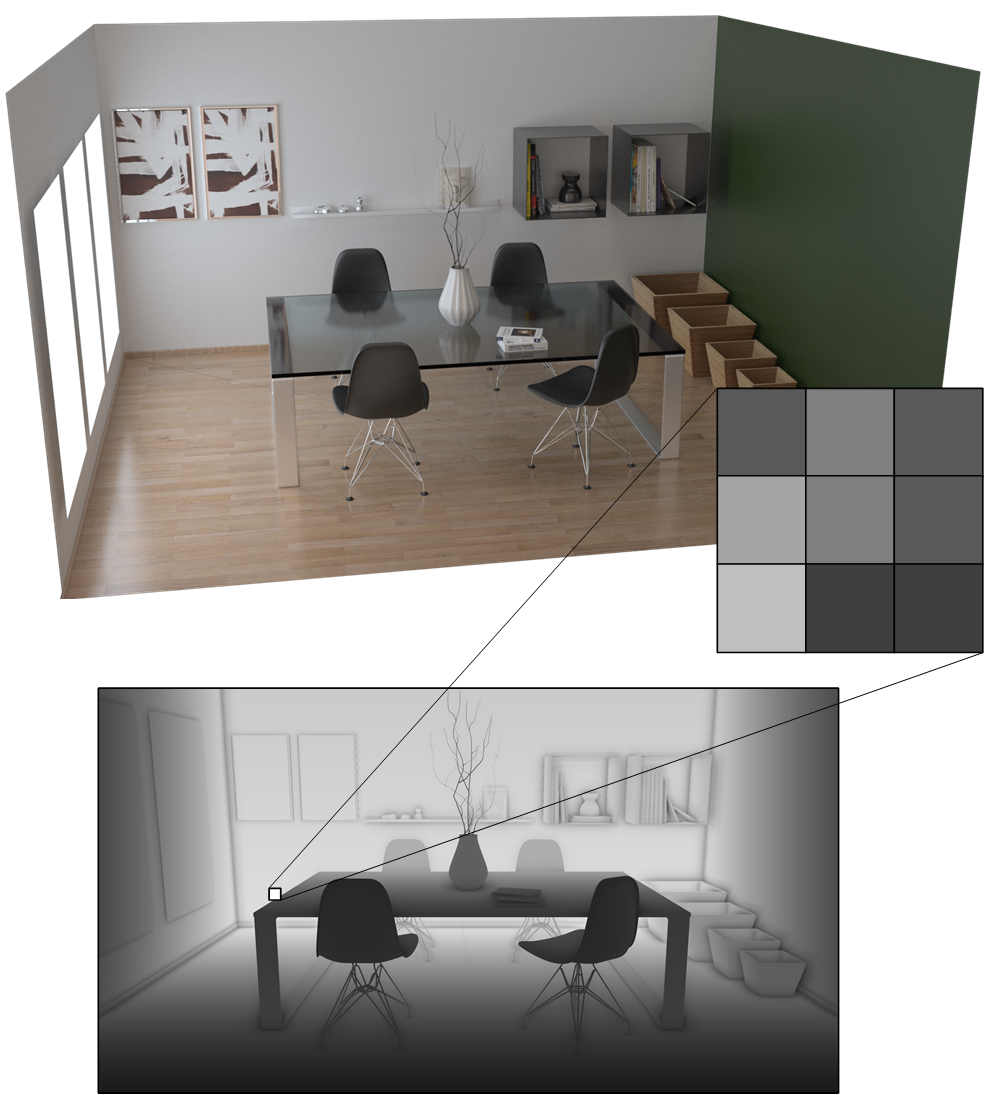
\includegraphics[width=\linewidth]{figs/lidar_simulation/depth_buffer.png}
	\caption{Depth buffer of a 3D scene, as proposed in previous LiDAR simulations. }
	\label{fig:depth_buffer_lidar}
\end{marginfigure}
Another key factor is the use of procedural 3D environments; scenes modelled by professionals can be utilized for generating a few datasets from several viewpoints, whereas those governed by generation rules lead to constructing large datasets from different environments. Besides TLS, which is by far the most studied kind of LiDAR sensor, this chapter is also intended for describing how to simulate aerial surveys considering both sensor errors and surface properties. In comparison with previous work, collisions are solved using state-of-the-art ray-tracing data structures, instead of solving it through a \textit{z}-buffer of limited resolution (Figure \ref{fig:depth_buffer_lidar}). Consequently, this piece of software is able to construct high-quality point clouds with low latency. Nevertheless, working in the image space is sometimes required; for instance, Deep Learning models are easier to operate in images than over 3D point clouds without losing precision on them (e.g., by voxelizing).

In comparison with previous work, the main contributions of this chapter are the generation of large labelled LiDAR datasets using procedural scenarios as input. These are obtained in a reduced response time, following a physically-based interaction, while a sequential approach requires several minutes, even hours, for solving complete scans of a whole target area. The complete procedure is depicted in Figure \ref{fig:lidar_overview}. 

\section{On the generation of synthetic LiDAR datasets}

LiDAR technology has rapidly evolved in the last two decades and therefore, it has received great attention from industrial and academic environments. This sensor enables acquiring information about a surface, object or phenomenon without physical contact. There is a wide variety of LiDAR variants according to the sensor capabilities, the platform on which they are operated, manufacturers and models. Some of these are TLS (terrestrial), ALS (aerial), MMS (mobile) and BMLS (backpack-mounted). Unfortunately, it is not easy to get a sufficient amount of ground truth data due to time constraints and available resources. In contrast to real LiDAR sensors, LiDAR simulation enables the generation of classified data at a significantly lower cost. The cost of LiDAR technology is prohibitive, and collecting large real-world datasets is time-consuming, both in the acquisition and labelling (if required). 

Synthetic LiDAR data can be accurately labelled since 3D environments modelled by professionals are named accordingly, thus allowing us to establish a surface classification. The LOD of this labelling is constrained by the modelling of input environments as well as by the requirements of decision-making and classification algorithms that will use these datasets. Also, it is possible to obtain more realistic data by simulating errors and limitations of LiDAR, whether they are systematic or random. Consequently, simulating the physical interaction of a LiDAR sensor with real-world surfaces is a non-trivial task that requires a high response time. 

\begin{figure*}
    \centering
    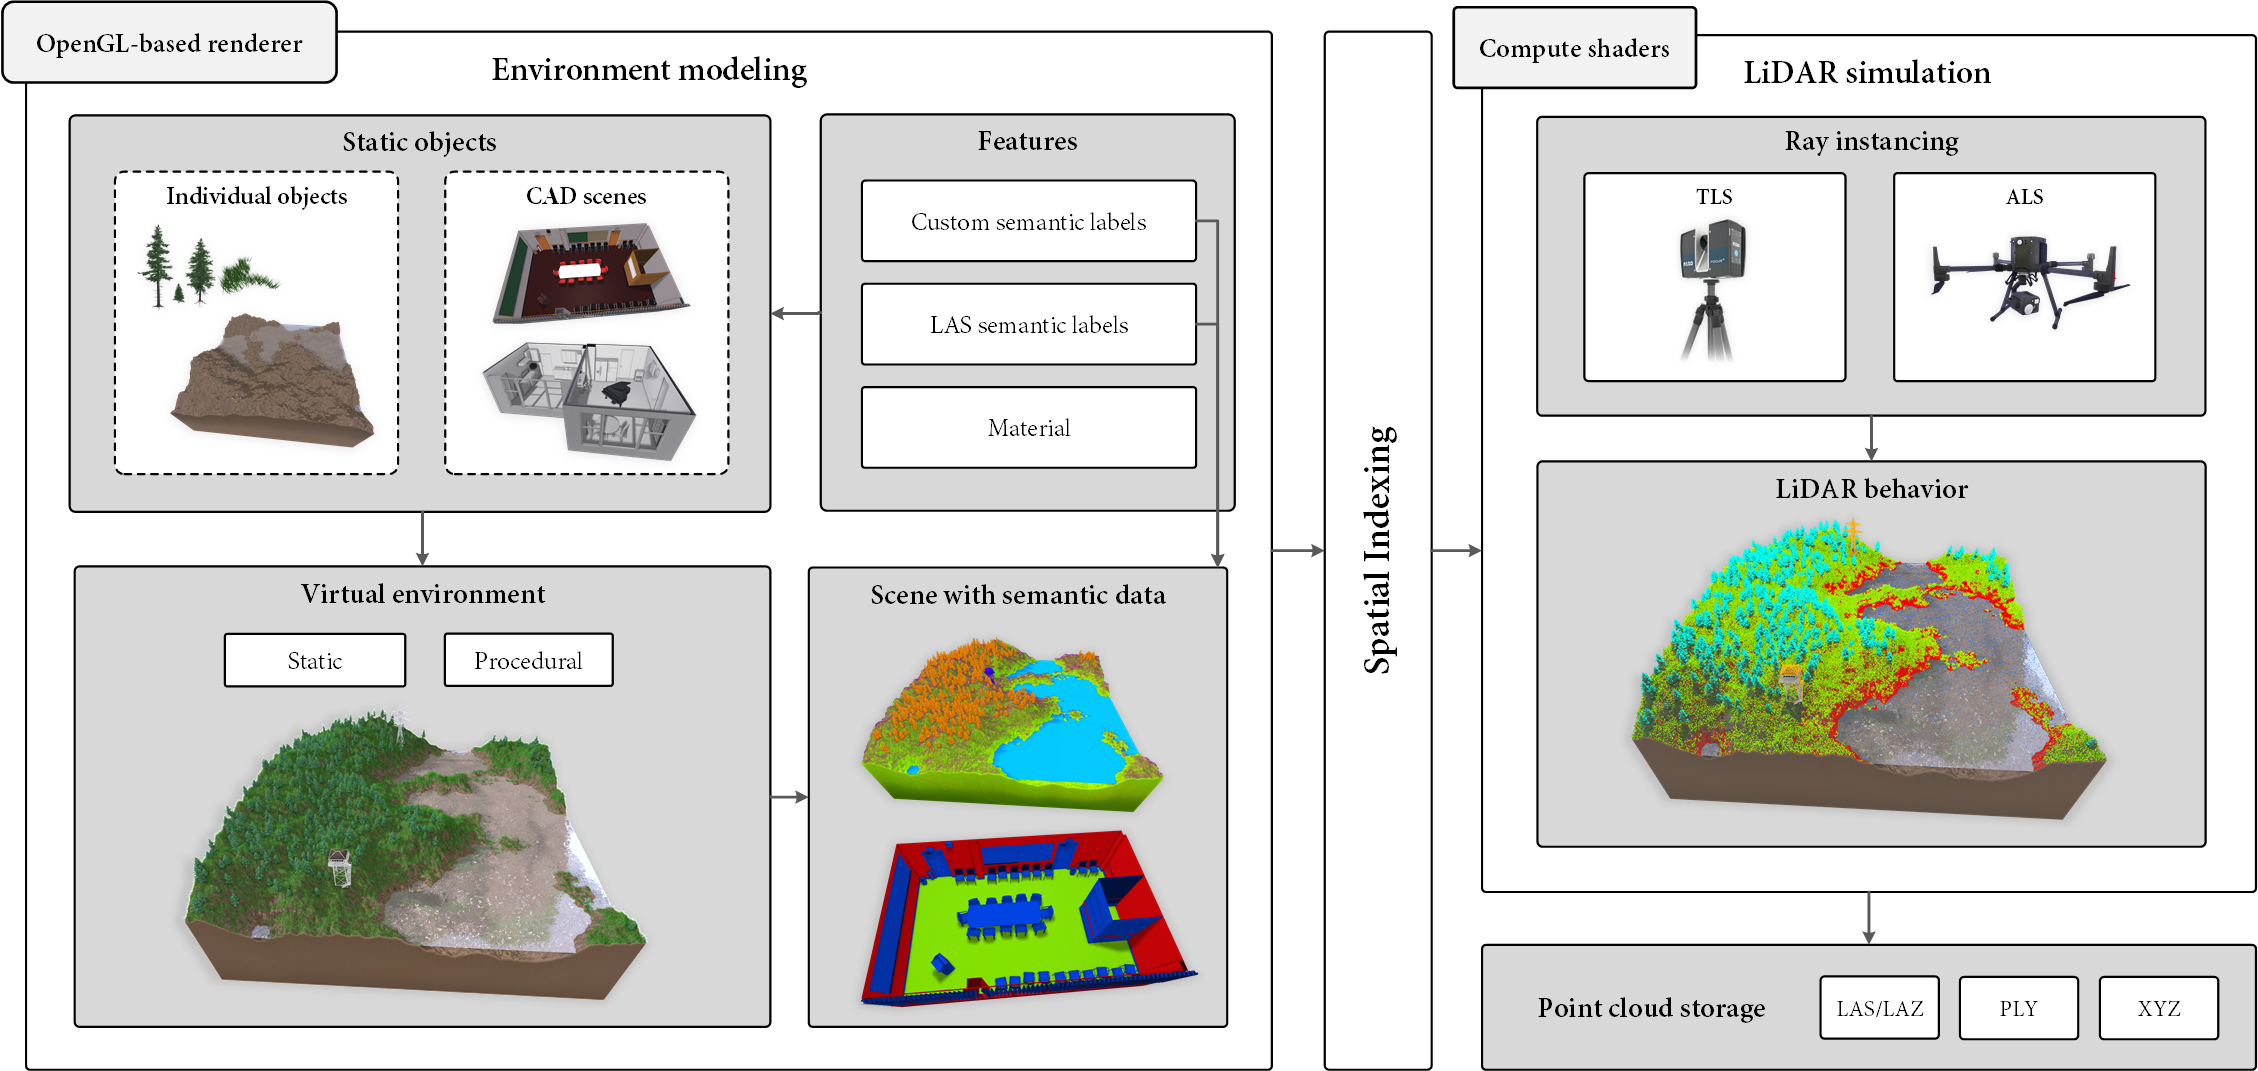
\includegraphics[width=\linewidth]{figs/lidar_simulation/overview.png}
	\caption{Overview of a LiDAR simulator operating over 3D virtual scenes, either procedural or static, which are previously indexed to speed up spatial queries. }
	\label{fig:lidar_overview}
\end{figure*}

\section{Modelling of synthetic environments}

Synthetic scenarios must be similar to real-world environments since the scanning results are aimed at feeding Deep-Learning algorithms. Furthermore, procedural scenarios are preferred over static ones in the generation of large datasets. Following this approach, the scenarios are modelled using rules over a collection of 3D models. In contrast to static scenarios, the labelling of procedural environments is more efficient as it is only performed once. Although third-party software exists for this task, such as SpeedTree\textregistered, a custom tool was implemented to meet our specific requirements and enable the labelling of every model instance. 

\begin{figure*}
    \centering
    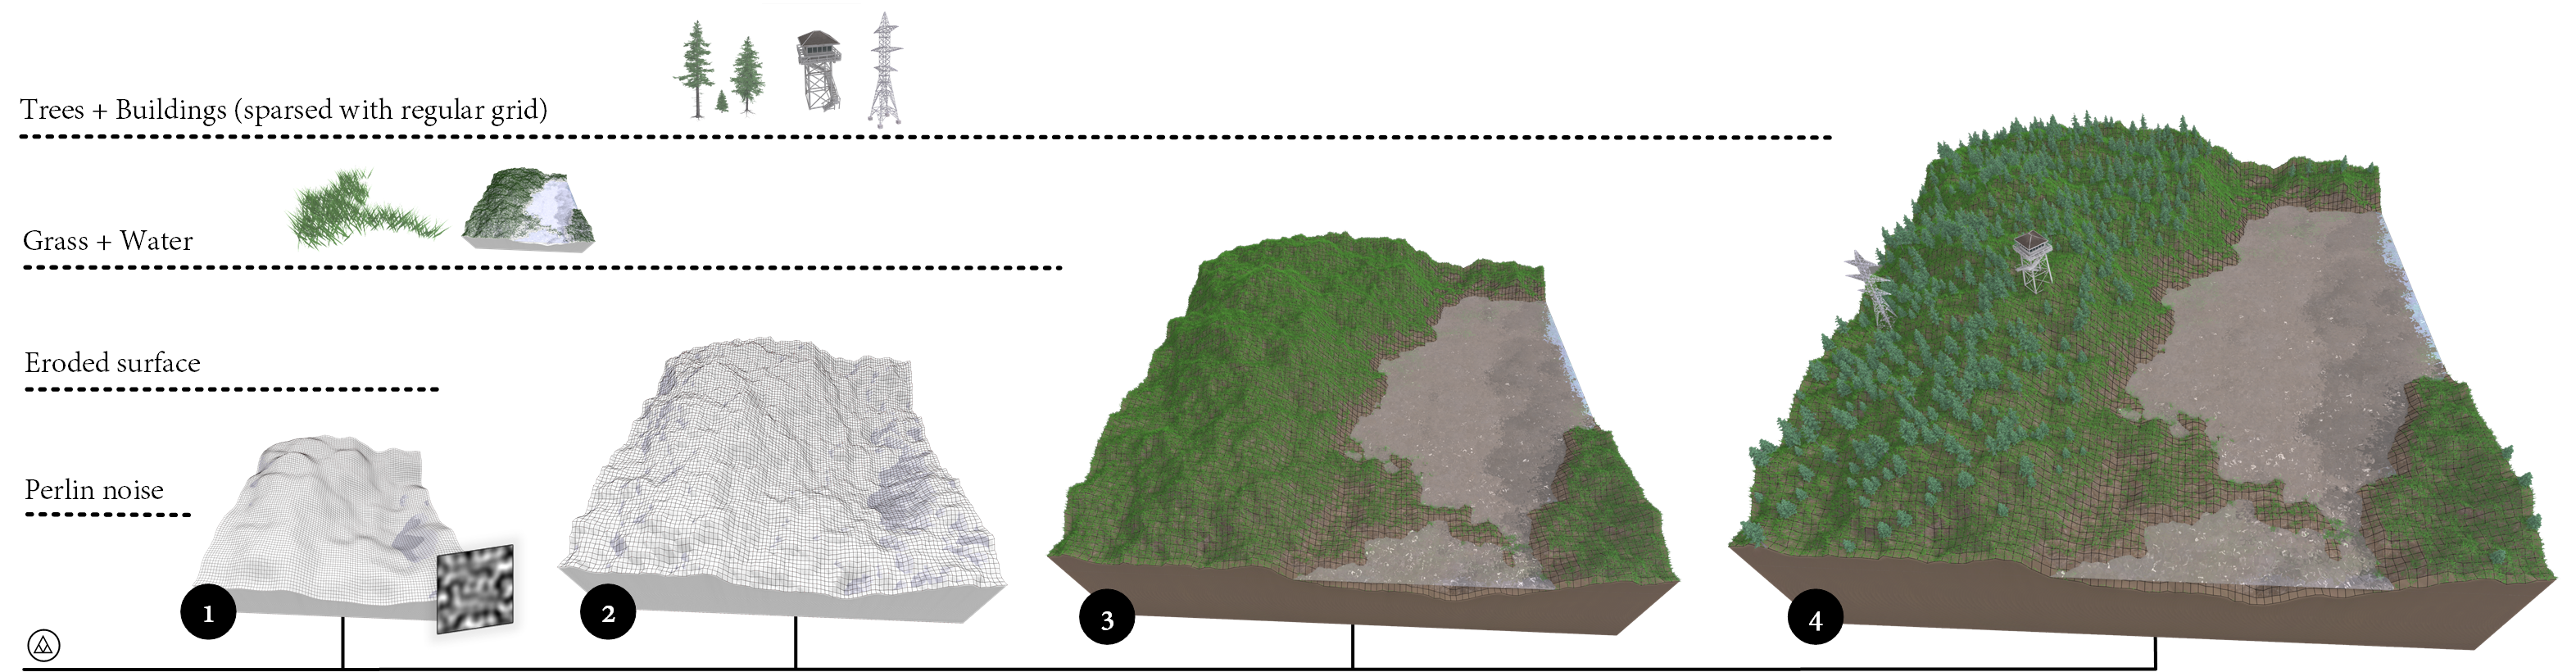
\includegraphics[width=\linewidth]{figs/lidar_simulation/procedural_workflow.png}
	\caption{Workflow regarding the procedural modelling of a forestry area with water, low-vegetation, high-vegetation and buildings. First, the soil is eroded using hydraulic processes, and then, water and low vegetation are procedurally generated. Finally, trees and buildings are generated so that collisions among them are avoided. }
	\label{fig:procedural_workflow}
\end{figure*}

\subsection{Forestry environments}

\begin{marginfigure}[.cm]
    \centering
    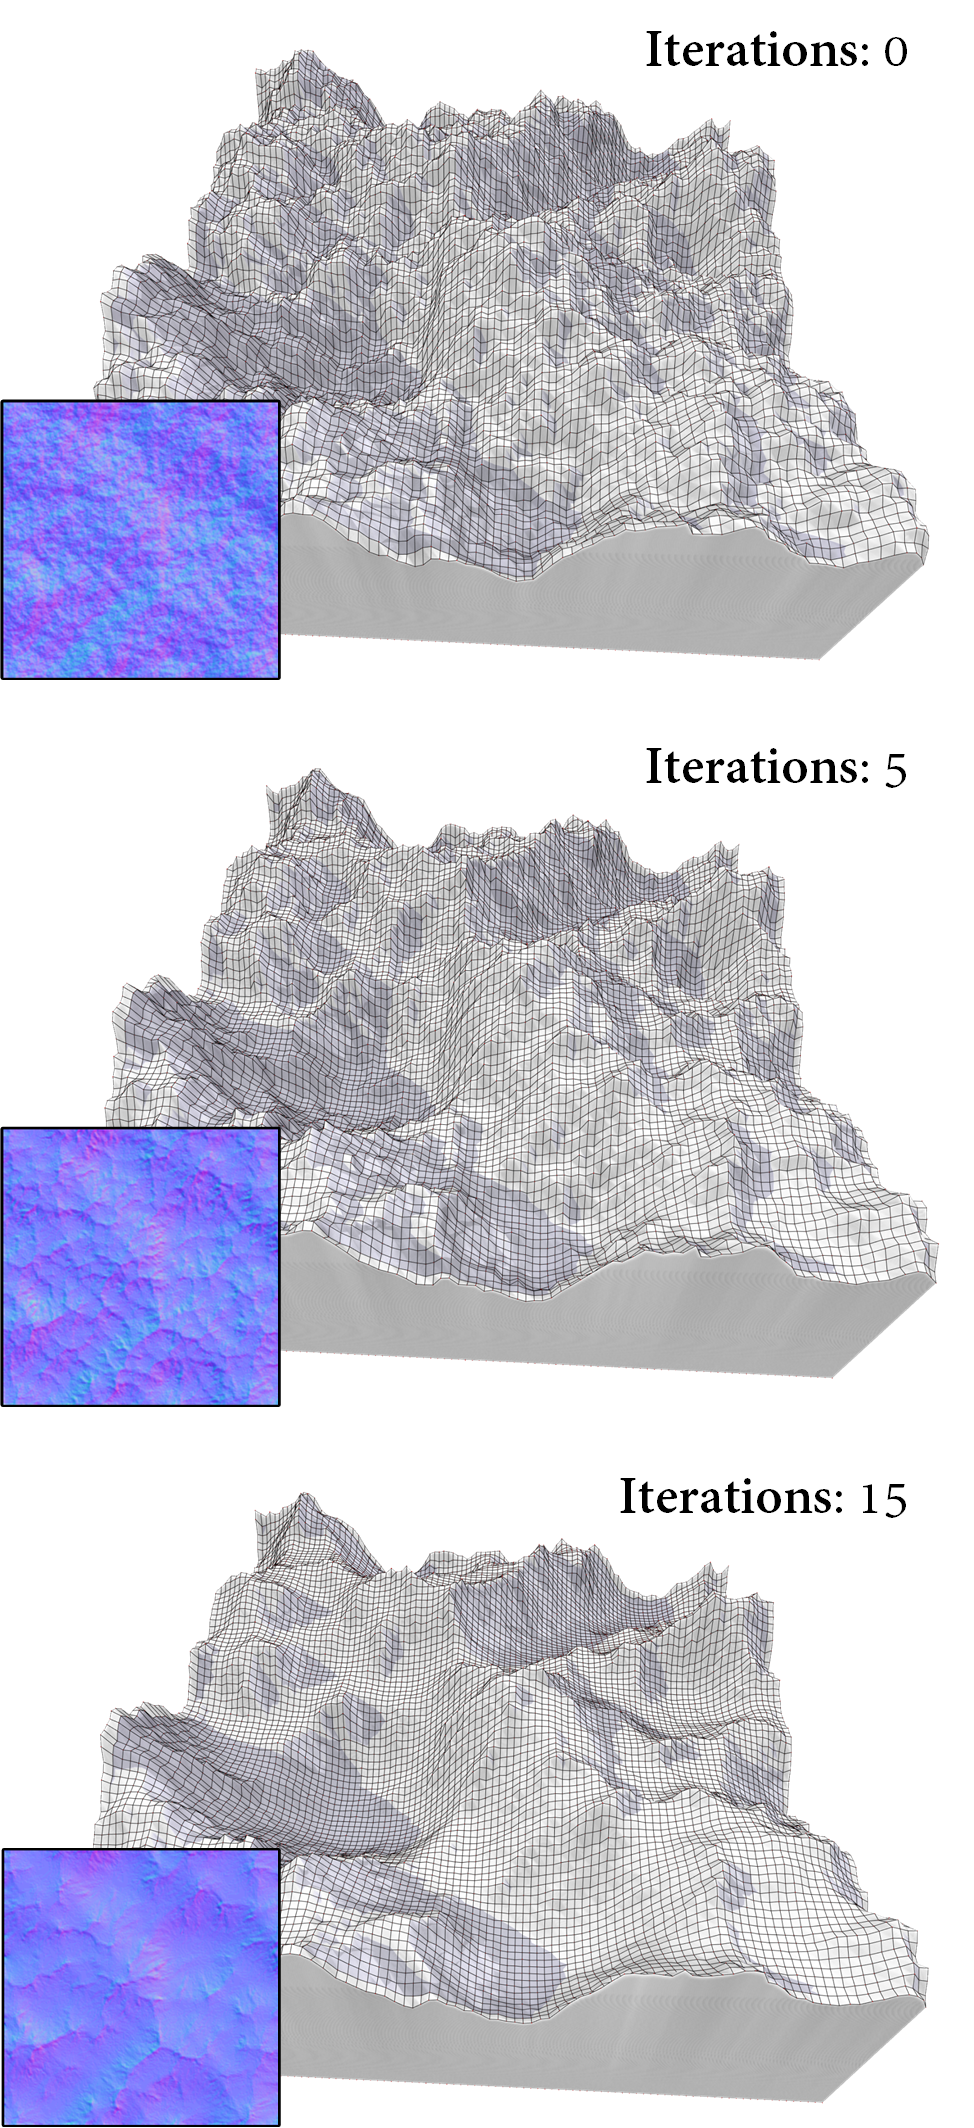
\includegraphics[width=\linewidth]{figs/lidar_simulation/erosion.png}
	\caption{Hydraulic erosion of 200k particles over a heightfield modelled with 2D Perlin noise. }
	\label{fig:hydraulic_erosion}
\end{marginfigure}
The procedural generation of forestry scenarios has been previously approached with ecosystems \cite{cordonnier_authoring_2017, fischer_autobiomes_2020, makowski_synthetic_2019} that achieve a high level of realism. However, this work intended to provide a simple tool for the procedural generation of this kind of scenarios, following the procedure in Figure \ref{fig:procedural_workflow}. These scenarios can be either configured using a text file or through a node editor in the graphic application.

The soil is modelled using a Perlin noise function, followed by hydraulic erosion over the heightfield representation of the terrain. The erosion algorithm was enhanced using the GPU to model each particle with a different thread. Accordingly, the particle moves are given by a weighted aggregation of slopes from a neighbourhood, until reaching a move of length zero or a limit of iterations, $\rho_{\textit{iterations}}$. During these moves, particles deposit sediment whether the carried material exceeds their capacity; otherwise, the heightfield is eroded. The erosion is applied over a radius as a convolution, with the weight $w_i$ being the distance to the kernel centre. Regardless of the particle position, the convolution has always the same weights and thus can be computed once and stored. Figure \ref{fig:hydraulic_erosion} shows several stages of this hydraulic erosion for 200k particles. The surface is smoother if the erosion runs for a larger number of iterations. Hence, it is necessary to balance realism and computational complexity with a limited number of iterations. 

\begin{marginfigure}[2.5cm]
    \centering
    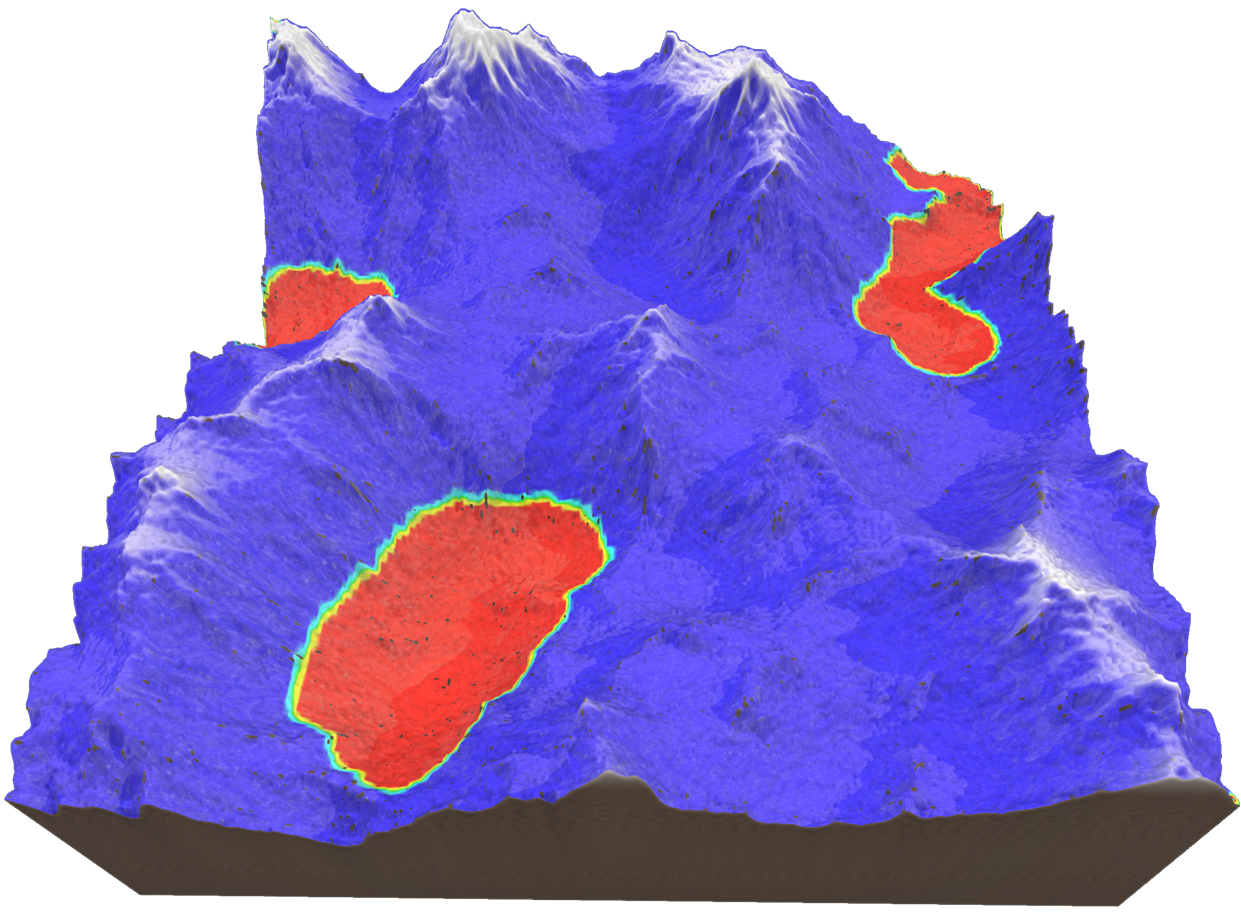
\includegraphics[width=\linewidth]{figs/lidar_simulation/valley_finds.png}
	\caption{Detected valleys on an eroded terrain. }
	\label{fig:terrain_valleys}
\end{marginfigure}
On the other hand, water is modelled as planar surfaces placed at valleys. Local minima are sought as points whose elevation is lower than surrounding pixels. Then, local minima seeds are flooded until the height $h_{\textit{flood}}$ is achieved, thus obtaining which cells are within a valley. $h_{\textit{flood}}$ is computed as shown in Equation \ref{eq:water_height} using a reference height, $h_{\textit{water}}$, and a random value in $[-h_{\textit{variance}}, h_{\textit{variance}}]$, both obtained from the scene configuration. From the set of collected valleys, the top-n instances sorted according to the covered area are included in the environment. 
\begin{equation}
    \label{eq:water_height}
    h_{\textit{flood}} = h_{\textit{water}} + f_{\textit{random}}h_{\textit{variance}}
\end{equation}
where $f_{\textit{random}} \in [-1, 1]$.

Low-vegetation is densely modelled with a large number of low-poly instances that enable the modelling of highly detailed scenes while keeping a good rendering performance. Nevertheless, OpenGL's instance rendering is required for providing a comfortable value of FPS. Although it can also be rendered using a geometry shader, the LiDAR simulation requires the vegetation geometry to be stored in an SSBO for the spatial indexing stage. These objects are distributed using seeds from a random uniform distribution, although the slope and height also influence whether they are instanced or not. This instancing probability is defined as shown in Equation \ref{eq:vegetation_instancing_prob}. The probability map is rendered in a texture by aggregating the height and normal map computed in previous stages. According to Equation \ref{eq:vegetation_instancing_prob}, points that present steeper slopes and lower altitudes have a lower instancing probability.
\begin{gather}
    \label{eq:vegetation_instancing_prob}
    p_{i, j} = 1 - w_{\textit{height}} \cdot H(h, h_{\textit{min}}, h_{\textit{max}}) - w_{\textit{slope}} \cdot (1 - \hat{n} \cdot \left[0, 1, 0\right]^\intercal)
\end{gather}
where $H(h, h_{\textit{min}}, h_{\textit{max}})$ is an Hermite interpolation function in $[h_{\textit{min}}, h_{\textit{max}}]$, and $\hat{n}$ is the normal vector at $(i, j)$, given that $i \in [0, \textit{width}[$ and $j \in [0, \textit{height}[$, with $\left(\textit{width}, \textit{height}\right)$ being the size of the eroded heightfield.

\begin{figure*}
    \centering
    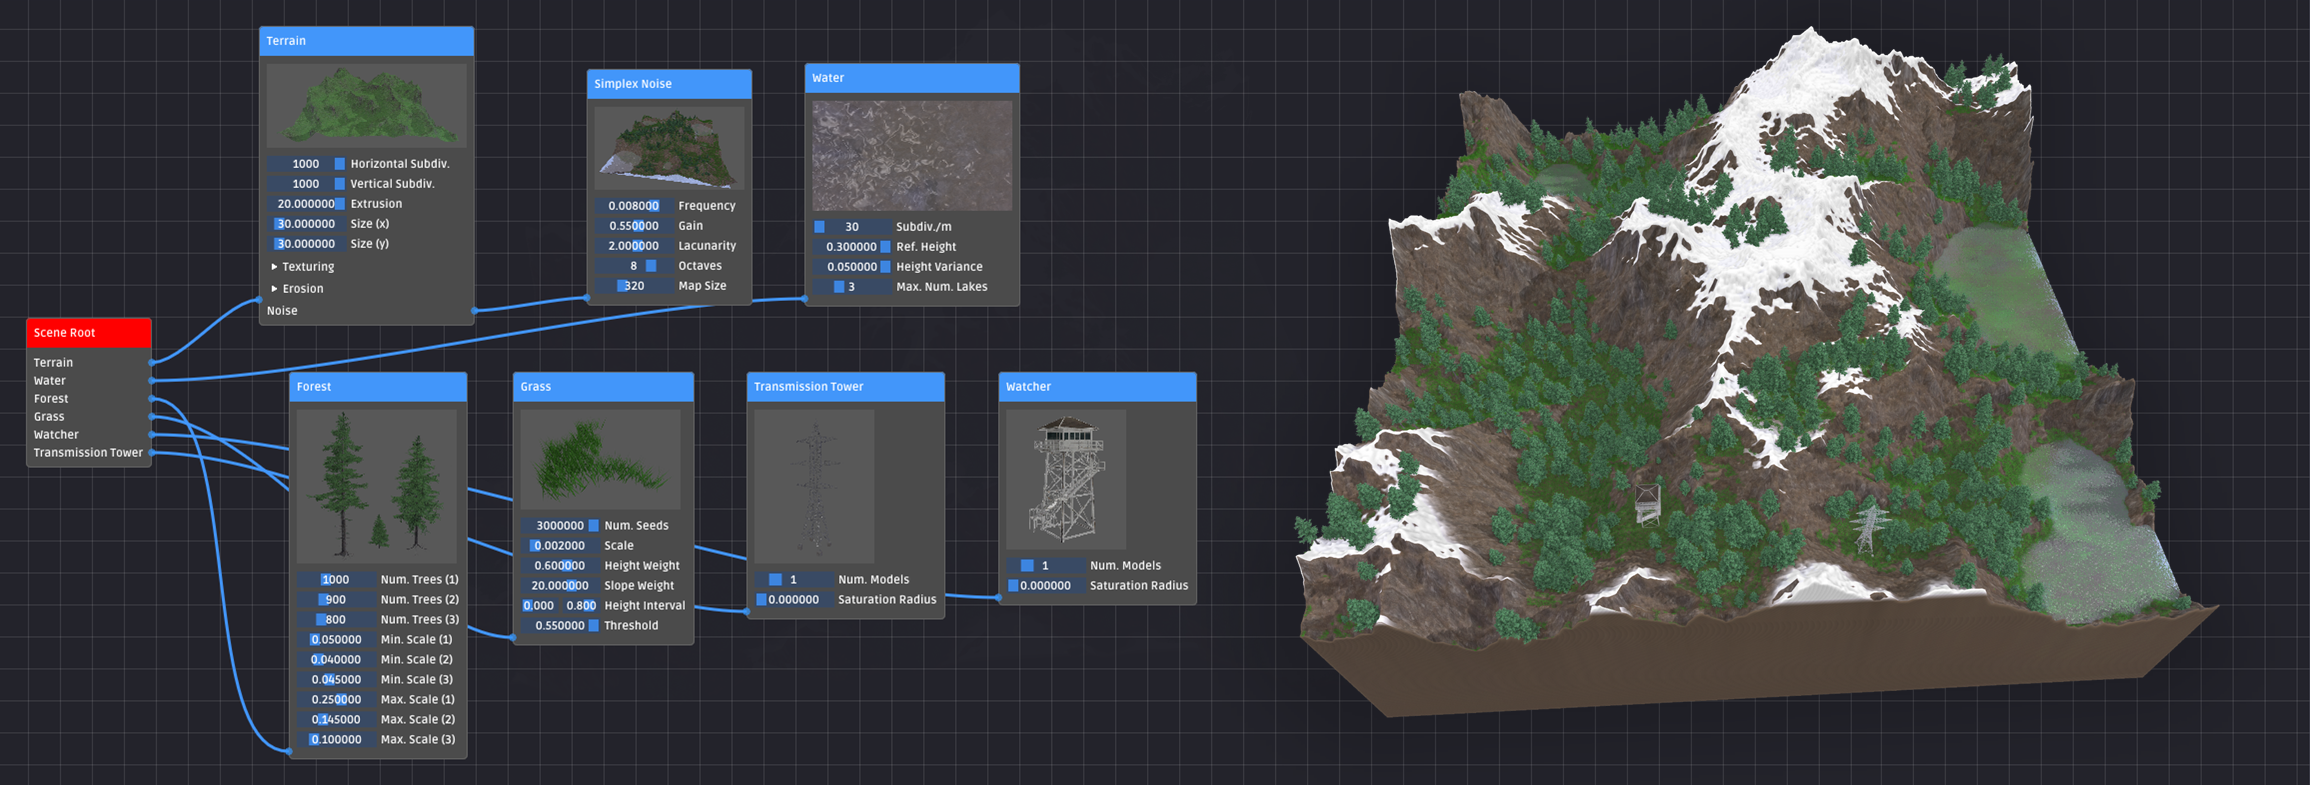
\includegraphics[width=\linewidth]{figs/lidar_simulation/node_editor.png}
	\caption{Node editor configuration for obtaining an environment such as the one depicted on the right side.  }
	\label{fig:node_editor}
\end{figure*}

In contrast to low vegetation, tree instancing considers the distribution of previously generated objects to avoid overlapping geometry. The triangle mesh collision tests were accelerated using a 2D regular grid rather than checking the polygonal meshes. Hence, this approach avoids using seeds in cells which are already occupied. Each time a new object is instanced, the target grid cell is saturated with a factor of $f_{\textit{sat.}}$ within a radius $r$. Then, a grid cell is considered to be saturated whether its occupation is over a threshold, $h_{\textit{sat.}}$. Accordingly, the vegetation density is controlled with the grid subdivision and $h_{\textit{sat.}}$. If a grid cell must be occupied by a single model, then it is assigned a value of $\infty$. 

\subsection{Urban environments}

Urban scenarios are partly modelled as procedural environments (see Figure \ref{fig:procedural_urban}). The baseline are large city and residential scenarios modelled by professionals, whereas pedestrians and vehicles are procedurally instanced. To this end, candidate seeds are sparsed over sidewalks and road models and instanced whether the linked random value is below a threshold. The instancing frequency as well as the varying scale of each model can be configured. 

\begin{marginfigure}[.cm]
    \centering
    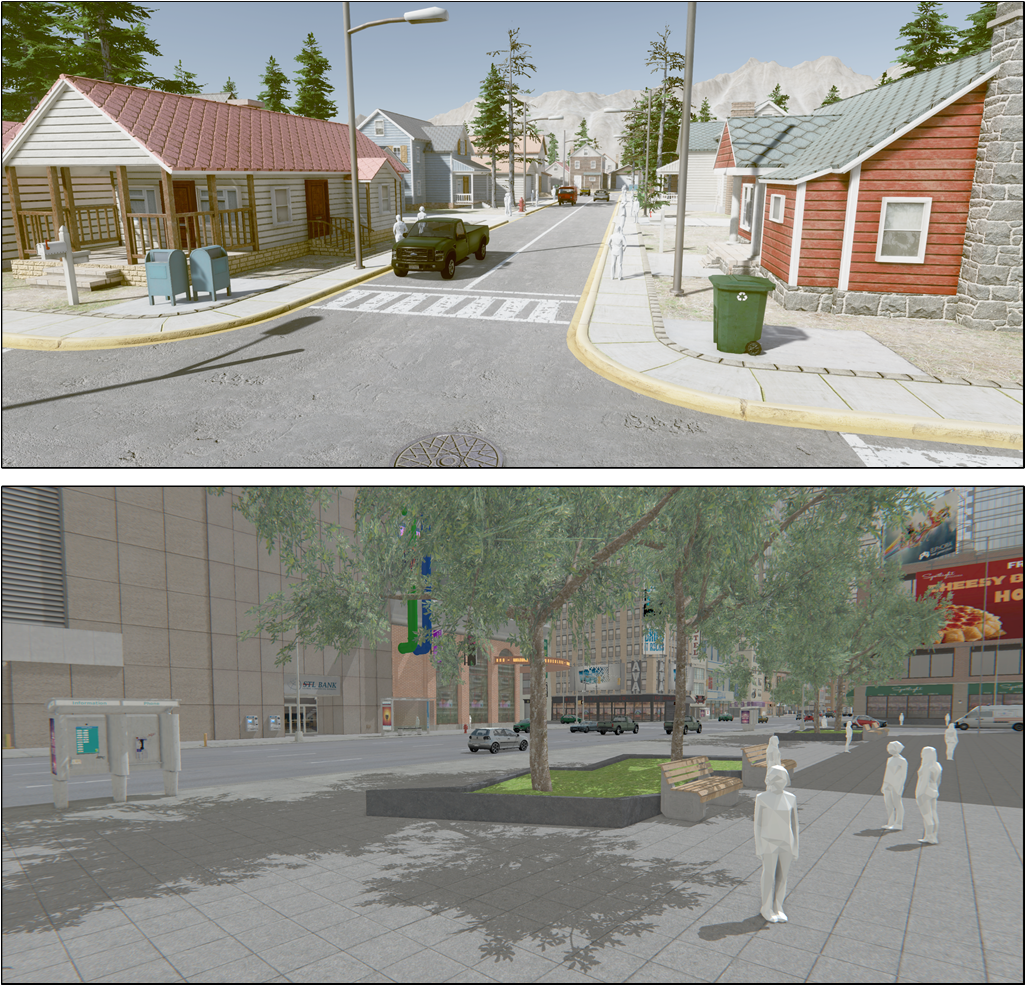
\includegraphics[width=\linewidth]{figs/lidar_simulation/procedural_urban.png}
	\caption{Procedural urban environments based on a) a residential area and b) a metropolis. }
	\label{fig:procedural_urban}
\end{marginfigure}
\begin{marginfigure} [8.cm]
	\centering
	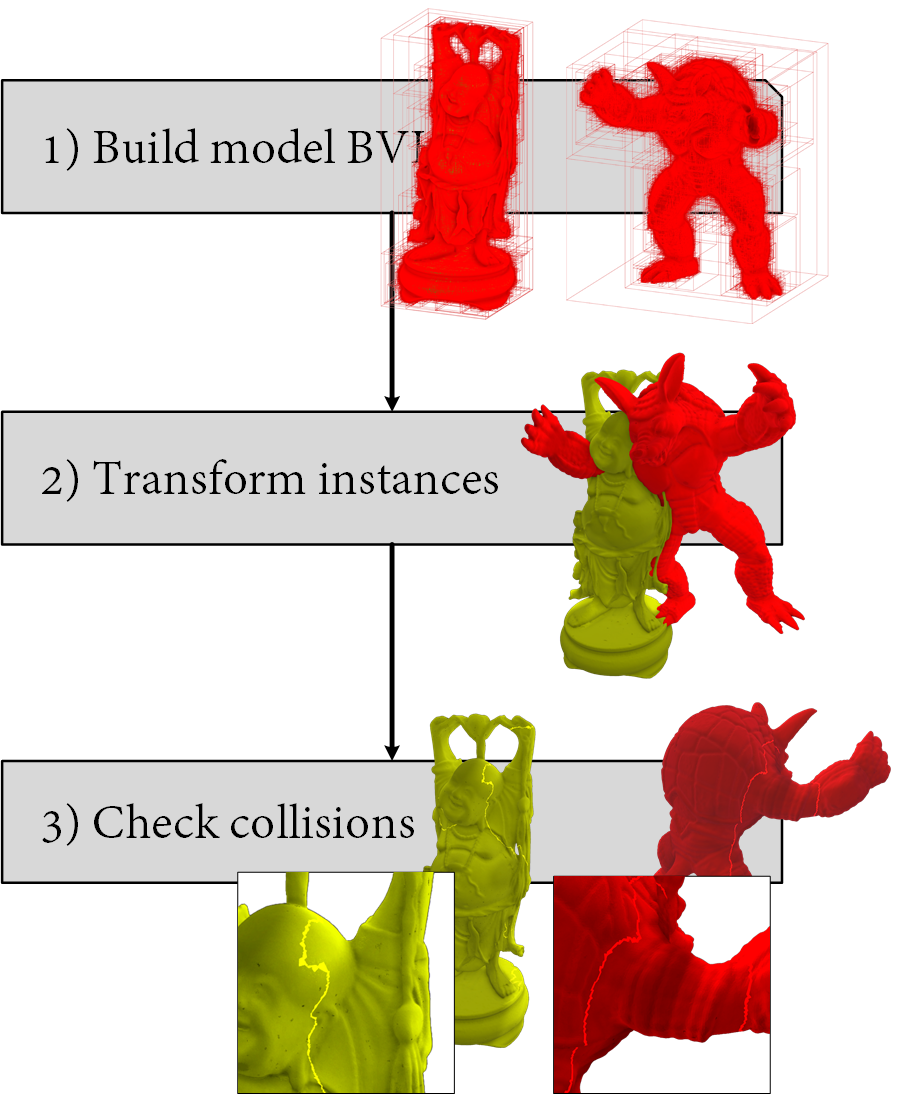
\includegraphics[width=\linewidth]{figs/lidar_simulation/mesh_collision.png}
	\caption{Detection of collisions between two triangle meshes. }
	\label{fig:triangle_mesh_collision}
\end{marginfigure}
Firstly, roads are split into rails according to their width, and then, vehicles are rotated using the road rotation matrix. The location is computed by selecting a random road and rail, as well as a random translation within it. On the other hand, the \textit{y} coordinate is computed as the collision of a ray emitted towards the road with $\textit{nadir}$ direction, plus half the height of the vehicle's bounding box. The main concern during the instancing of vehicles is to avoid inter-collisions. Hence, these can be detected by building the BVH of each different model and rapidly solving if there are collided polygons. However, doing this for every instance is very time-consuming; instead, BVHs are built for every model in the database, and they can be transformed according to the instance's transformation matrix. Still, transforming every vertex is time-consuming, and thus, collisions between triangles can be identified by casting rays with the shape of the edges of every source model's triangle. Thus, three rays are cast for every triangle, with its coordinates being transformed as shown in Equation \ref{eq:mesh_collision_ray}. Rather than comparing the new instance with the rest, it is narrowed using a 2D regular grid whose subdivision length corresponds to the maximum \textit{xz} length from any collected vehicle. Similarly, the source model from which rays are emitted is selected as the one with the lower number of polygons.
\begin{gather}
    \label{eq:mesh_collision_ray}
    \begin{aligned}
        r_{o} &= \inv{C_{T}} \cdot C_{S} \cdot v_{\textit{origin}}\\
        r_{t} &= \inv{C_{T}} \cdot C_{S} \cdot v_{\textit{target}}\\
        r_{d} &= \widehat{r_{t} - r_{o}}
    \end{aligned}
\end{gather}
where $r_{o}$, $r_{t}$ and $r_{d}$ are the ray's origin, target and direction, and the vertices $v_{\textit{origin}}$, $v_{\textit{target}}$ are part of a triangle edge. Composite matrices ($C$) with $T$ subscript correspond to the target model, whereas $S$ refers to the source instance, i.e., the model with a lower number of polygons.

On the other hand, translation and rotation vectors are significantly more randomized for pedestrian instancing. Pedestrian models are randomly selected, whereas their location and rotation in the $y$-axis are described using three random values ($t_x$, $t_z$, $r_y$). As proposed before, the $y$ coordinate can be obtained by casting a ray with $\textit{nadir}$ direction. The detection of inter-collisions is addressed as explained, though pedestrians may also collide with buildings. Thus, it requires building the BVH of non-populated urban objects. Finally, procedural trees are also generated in some areas, and they can be upscaled and downscaled within a user-defined interval.

\section{Spatial indexing}

The objective of our synthetic LiDAR is to generate accurate returns. To this end, these are computed with ray-casting in 3D, rather than solving it in the image space. However, highly detailed scenarios are composed of several millions of triangles, whereas the LiDAR must also emulate millions of rays. Despite ray-triangle collisions being efficiently solved in the GPU, spatial traversal is the main concern and is considerably more time-consuming. Thus, this is a well-known time bottleneck even for optimized proposals. 

\begin{marginfigure}[.cm]
    \centering
    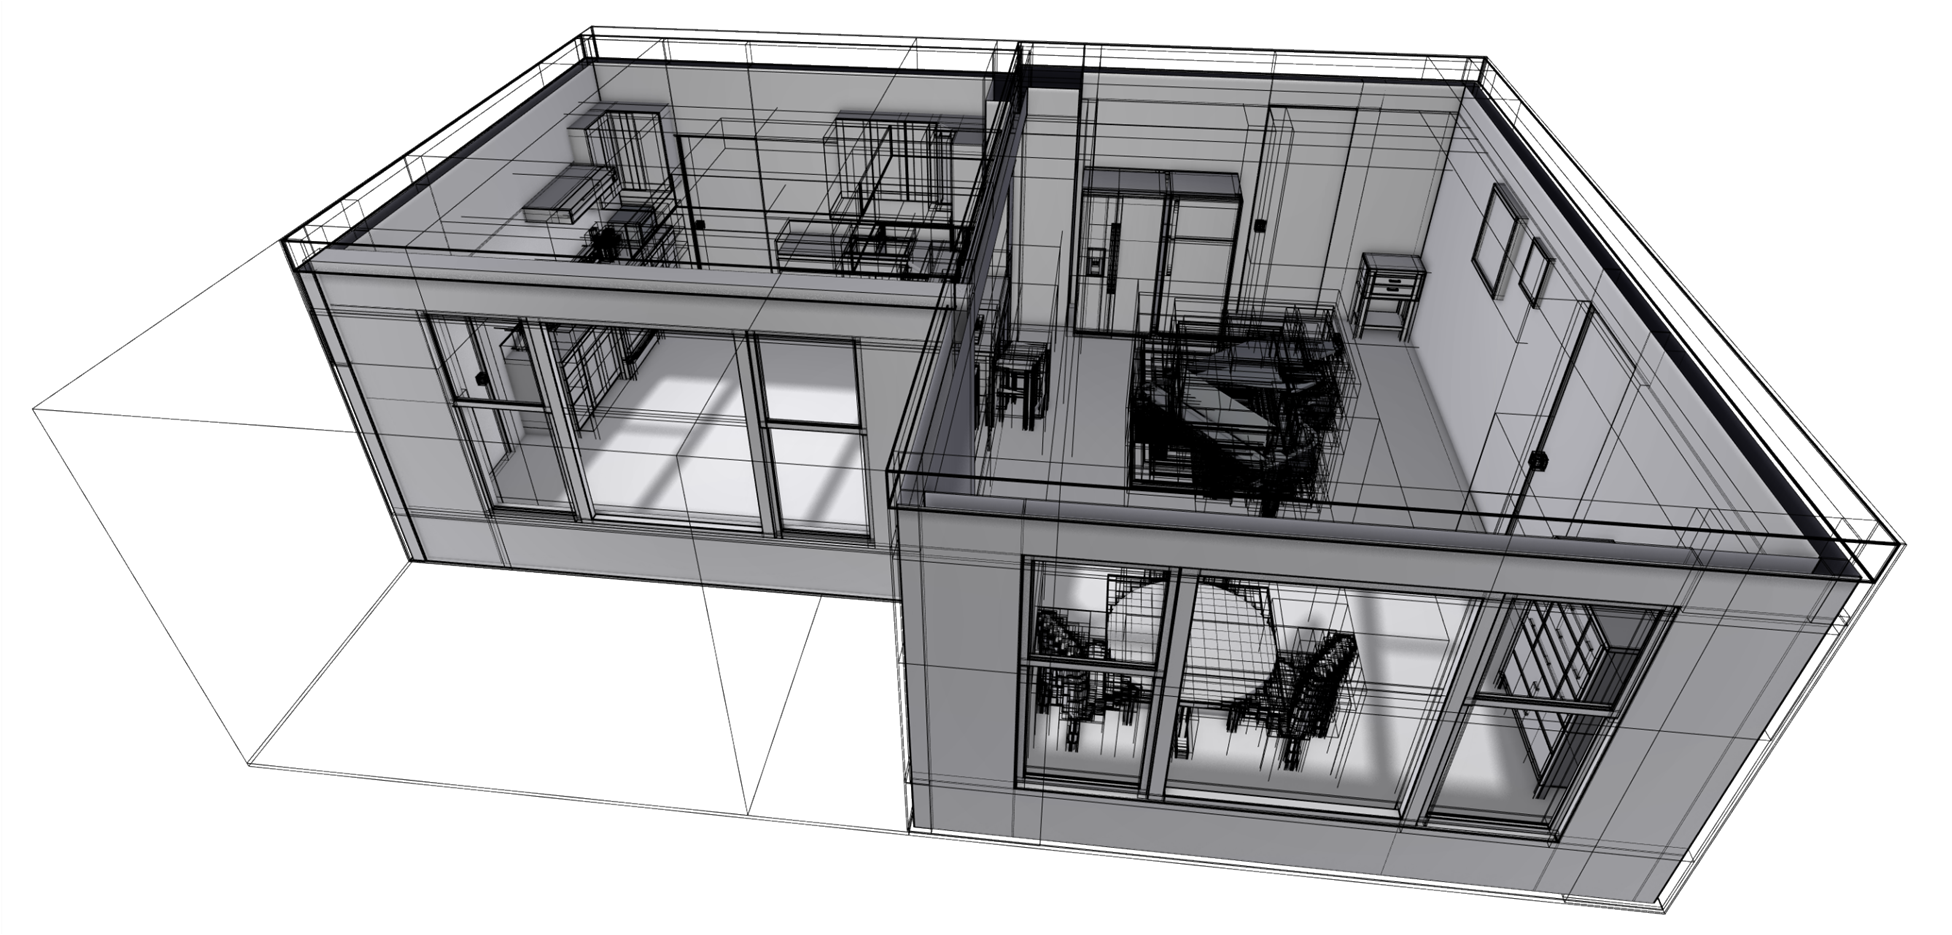
\includegraphics[width=\linewidth]{figs/lidar_simulation/bvh_rendering.png}
	\caption{Rendering of the BVH indexing of the very same scene in \ref{fig:kitchen_classification}. It was constructed using a buffer radius, $r$, of size 100.}
	\label{fig:lidar_bvh_rendering}
\end{marginfigure}
Either static or procedural, scenarios are indexed using a BVH, over which a large number of rays can rapidly traverse to solve millions of ray-triangle collisions. The indexing was performed as proposed by Meister and Bittner \cite{meister_parallel_2018} in the GPU. Hence, it is efficiently generated and after this, the BVH is stored in the GPU's memory to solve the subsequent scans, thus avoiding time-consuming transfer between CPU and GPU. This GPU-based approach enables building a BVH for ten million triangles with a response time below 1\si{\second}, as shown in Table \ref{table:bvh_response_time}. On the other hand, the traversal takes up a substantial portion of time, which can be reduced by making several threads work in parallel. The naïve traversal starts by the root and descends into the tree while pushing nodes into a stack. Hence, the topmost node of this stack is checked for intersections; the ray-AABB is rapidly solving with the algorithm proposed by Majercik et al. \cite{majercik_ray-box_2018}, whereas leaf nodes are checked with the ray-triangle test described by Möller \cite{moller_fast_1997}.

\section{Labelling of 3D triangle meshes}

\begin{marginfigure}[1.5cm]
    \centering
    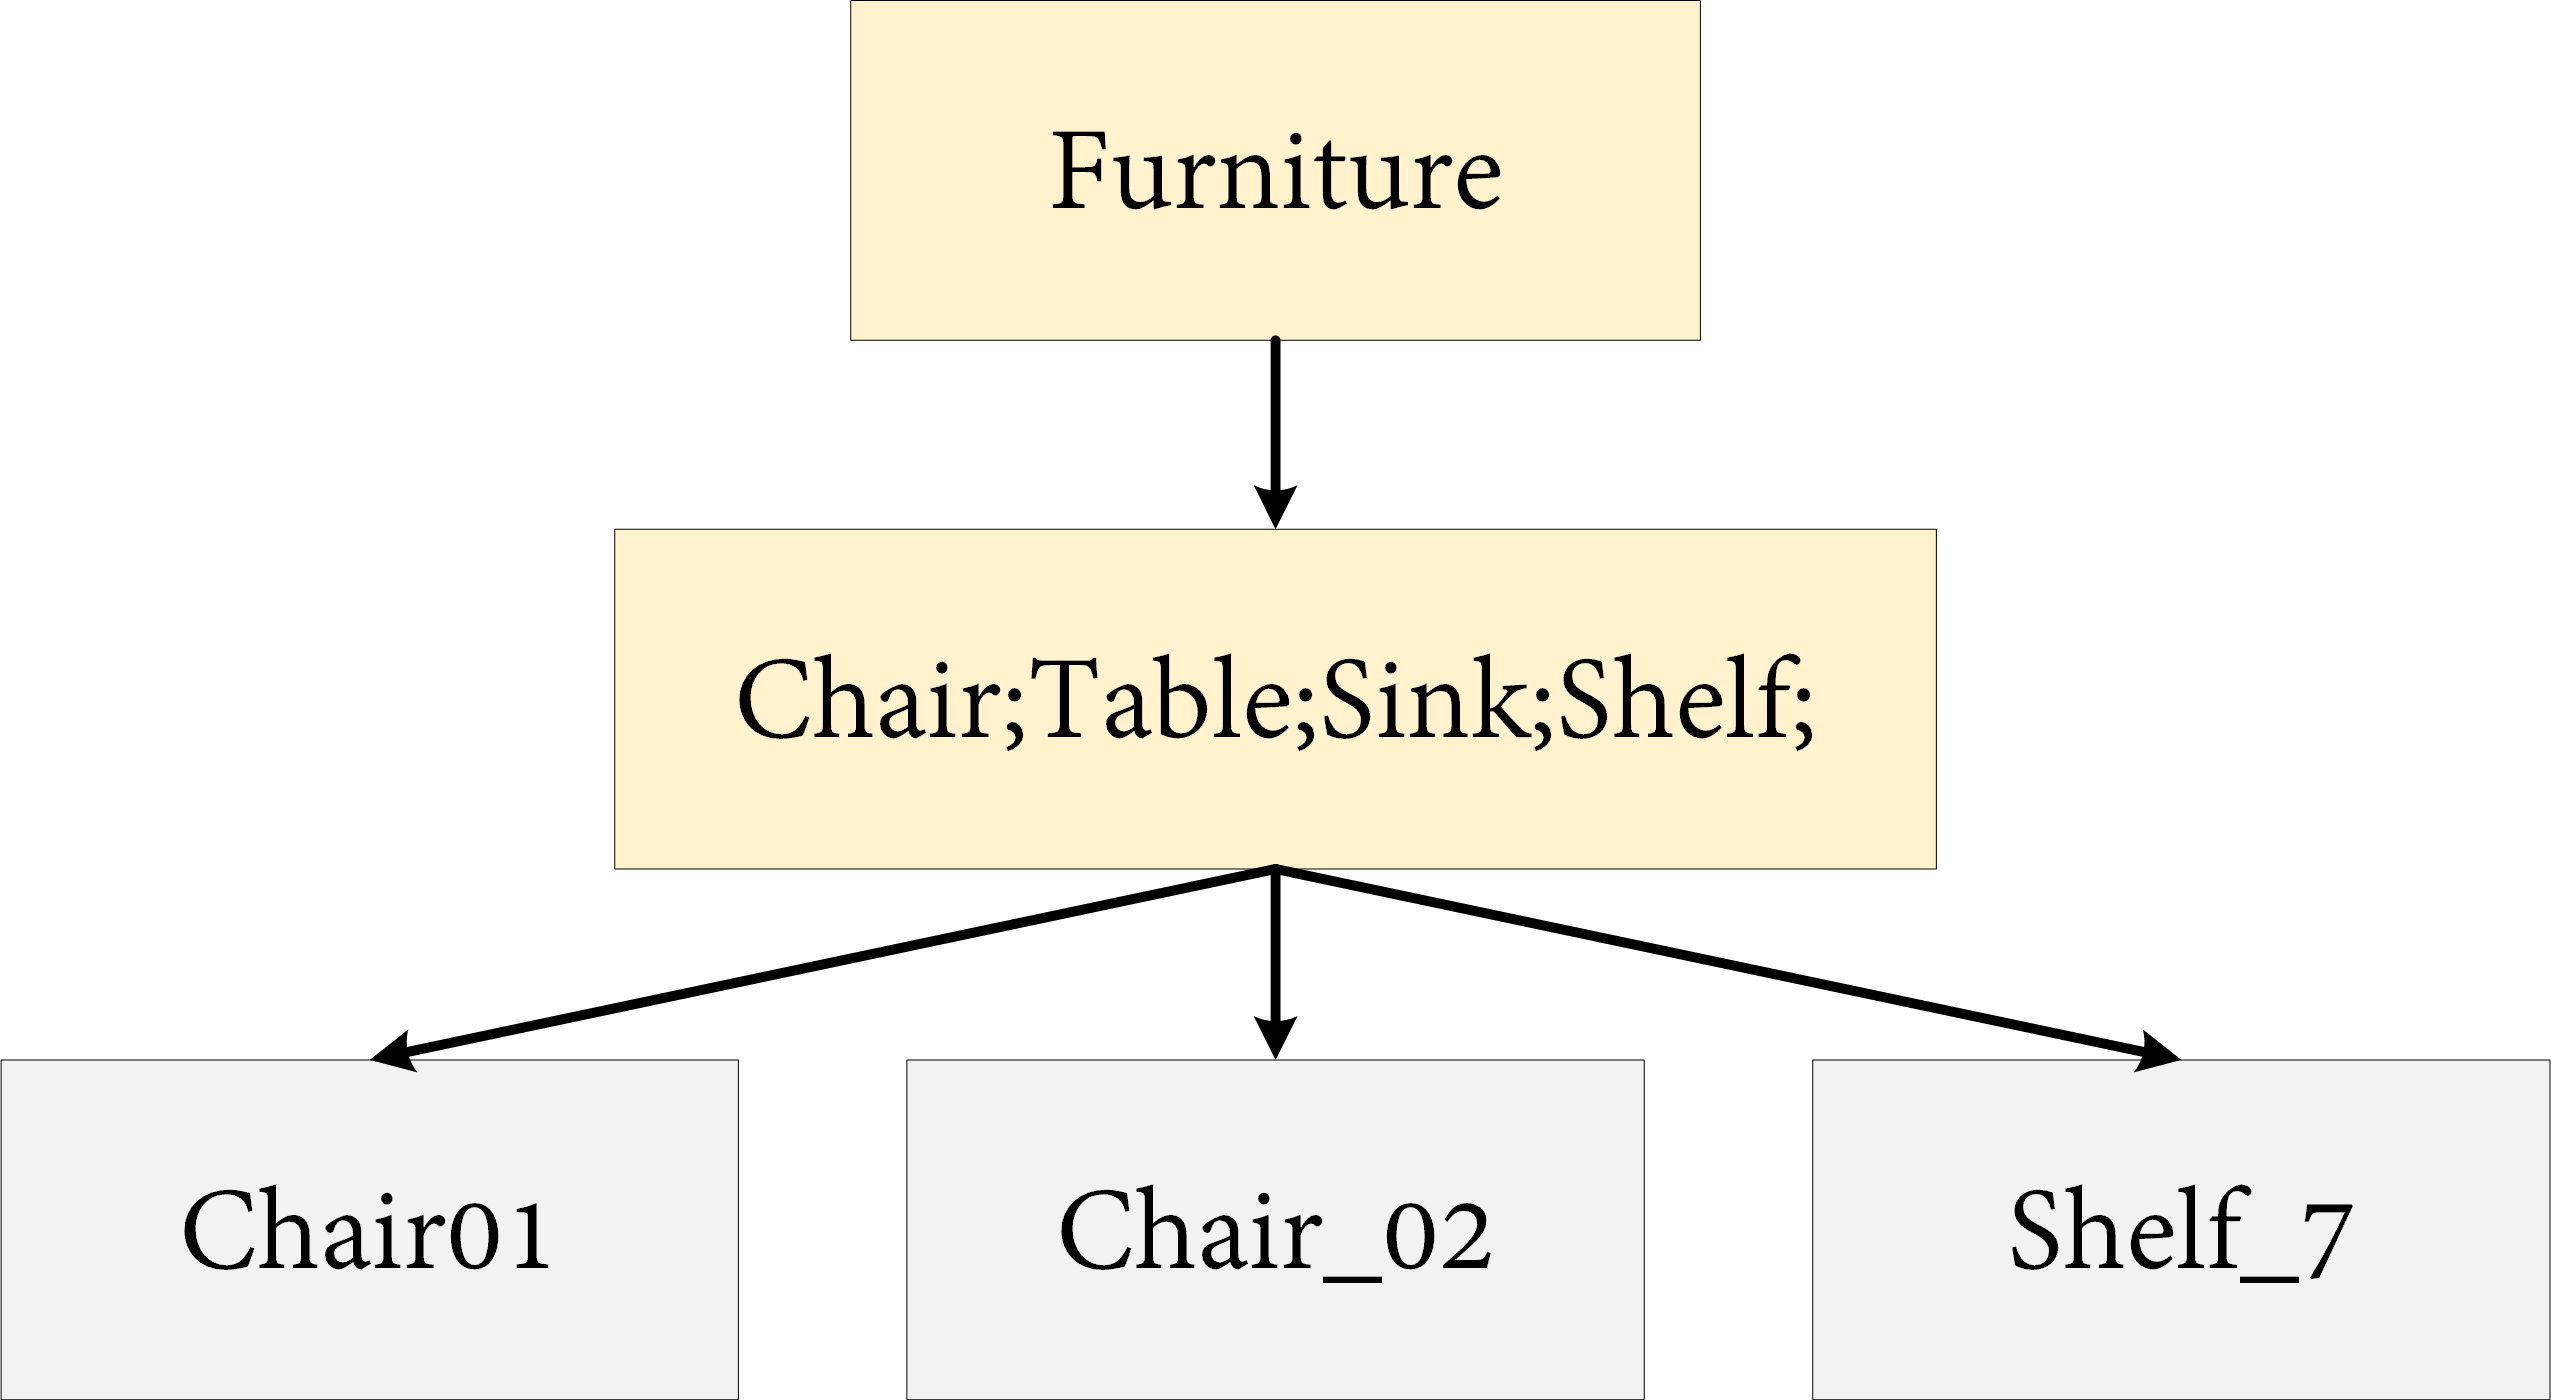
\includegraphics[width=\linewidth]{figs/lidar_simulation/semantic_labels_example.png}
	\caption{Example of hierarchical annotation: furniture tag includes a wide range of objects. }
	\label{fig:semantic_label_examples}
\end{marginfigure}
Instead of manually labelling large LiDAR point clouds, human operators are required to label models in triangle models. This task is facilitated using a hierarchical segmentation that is sped up using the naming conventions of objects and materials (see Figure \ref{fig:semantic_label_examples}). During the mesh loading, object names are considered significant whether they do not collide with other instances' names. Otherwise, they are named after the material together with a unique $\mathtt{id}$. Furthermore, models are organized either by following a custom tag or standard labels defined in the LAS file format (see Figure \ref{fig:kitchen_classification}). The former can be collapsed or further subdivided according to the required LOD, thus helping to provide a fine-grained segmentation. In contrast to the manual classification of real LiDAR point clouds, annotated environments help to suppress labelling errors and provide a fine-grain segmentation. Otherwise, manual labelling is limited to a few classes to avoid overwhelming human operators in this task.

\begin{figure}[ht]
    \centering
    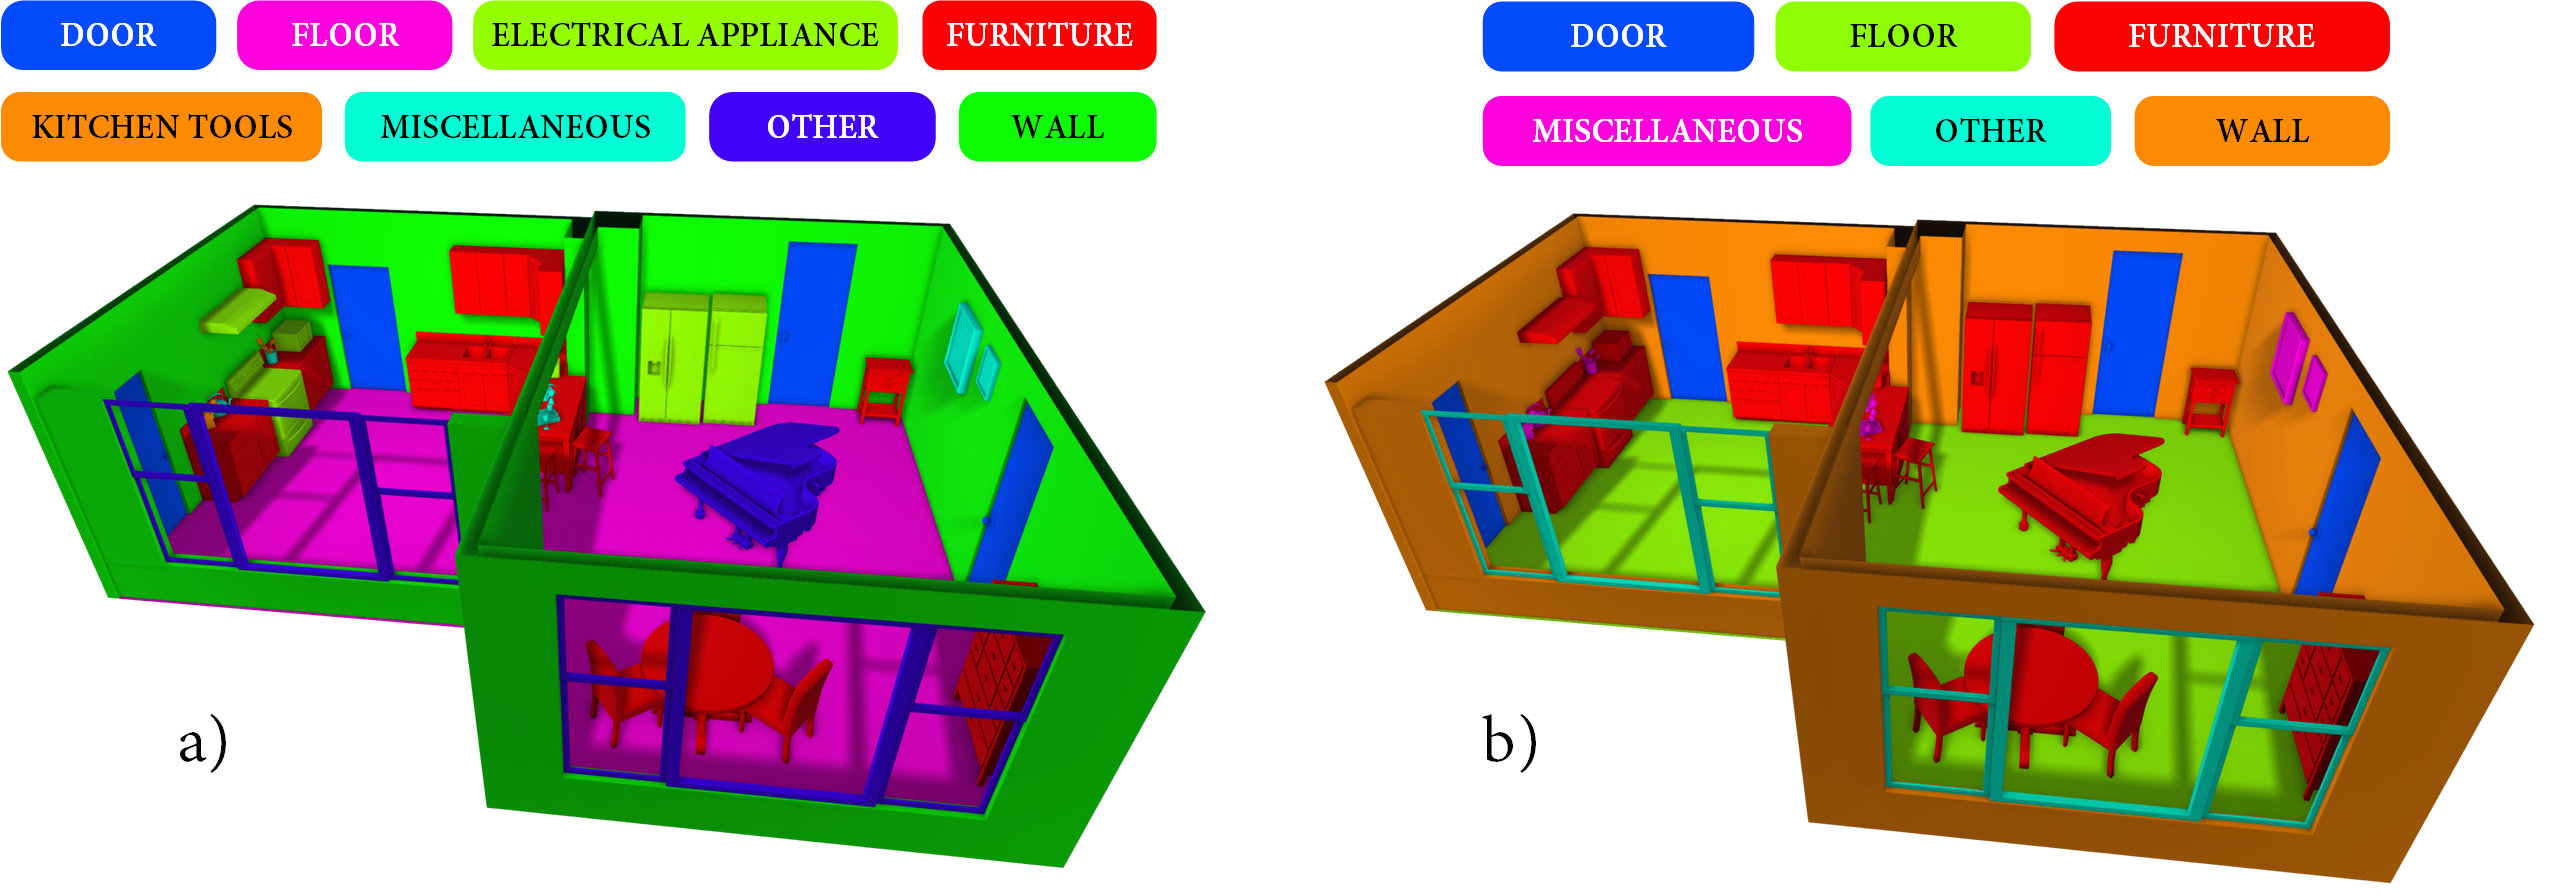
\includegraphics[width=\linewidth]{figs/lidar_simulation/semantic_labels.png}
	\caption{Different criteria for labelling a static scenario. First, the scene is annotated using custom labels, whereas the second classification is done according to the LAS 1.4 standard.}
	\label{fig:kitchen_classification}
\end{figure}

Besides semantic labels, models are also linked to materials that help in computing the LiDAR intensity. This property will be further described in the following chapter. Finally, the ID of each instance is also stored to make our datasets appropriate for instance segmentation.

\section{LiDAR simulation}

This section is structured according to the steps followed in the GPU-based LiDAR scans. First, a comprehensible explanation of LiDAR pulse modelling is given, followed by the interaction of LiDAR and synthetic surfaces. The latter stage also helps to introduce the pipeline in the GPU. 

\renewcommand{\arraystretch}{1.2}
\begin{table*}
    \small
    \centering
    \caption{Configuration parameters to propagate laser beams from a terrestrial LiDAR. Positional factors are expressed in meters, whereas angular parameters are expressed in radians.}
    \label{table:tls_parameters}
    \begin{tabular}{ll}
    \toprule
    \textbf{Parameter} & \textbf{Description} \\
    \midrule
    Position ($p$) & Position of LiDAR's emitter.\\
    Field of view ($\alpha_{\textit{fov}_{xz}}$, $\alpha_{\textit{fov}_{y}}$) & Aperture in both horizontal and vertical axis ($0 \leq \alpha_{\textit{fov}_{xz}} \leq 2\pi$ and $0 \leq \alpha_{\textit{fov}_{y}} \leq \pi$). \\
    Scanning resolution ($r_{x}$) & Number of horizontal scan lines. \\
    Horizontal reference angle ($\alpha_{\textit{centre}_{xz}}$) & It helps to calculate the starting angle of the horizontal axis as $\alpha_{\textit{centre}_{xz}} - \alpha_{\textit{fov}_{xz}} / 2$. \\
    Vertical reference angle ($\alpha_{\textit{centre}_{y}}$) & It helps to calculate the starting angle of the vertical axis as $\alpha_{\textit{centre}_{y}} - \alpha_{\textit{fov}_{y}} / 2$. \\
    The number of channels ($n_{c}$) & Number of simultaneous channels. \\
    Channel spacing ($d_{c}$) & Interleaved distance between consecutive channels.\\
    Channel angular distance ($d_{\alpha_{c}}$) & Interleaved emission angle between consecutive channels.\\
    Axis noise ($\hat{\delta}_{\textit{noise}}$) & Magnitude of ray jittering. \\
    Angle noise ($\alpha_{\textit{noise}}$) & Magnitude of the angle used for jittering the ray's target position. \\
    \bottomrule
    \end{tabular}
    \libertineNormal
\end{table*}
\renewcommand{\arraystretch}{1}

\subsection{Pulse modelling}

LiDAR pulses are represented as a set of rays emitted at the sensor's location and propagating towards the uniformly sampled points from a unit sphere. From now on, the sensor emitter will also correspond to the receiver to simplify the conceptualization of the LiDAR mechanism. Rather than a single ray, the physical behaviour of a LiDAR pulse is better simulated with multiple rays \cite{zohdi_rapid_2020} (see Figure \ref{fig:pulse_radius_insight}) within a radius that can be static (collimated beams; parallel rays) and dynamic (diverging beams). Rays in the same pulse are calculated according to the orthonormal basis ($\hat{u}, \hat{v}, \hat{r}_{d}$) formed by the ray direction and the $\hat{\textit{up}}$ vector. $\hat{u}, \hat{v}$ are then scaled with random numbers to generate points in a circumference of radius $p_r$. 

\begin{figure}
	\centering
	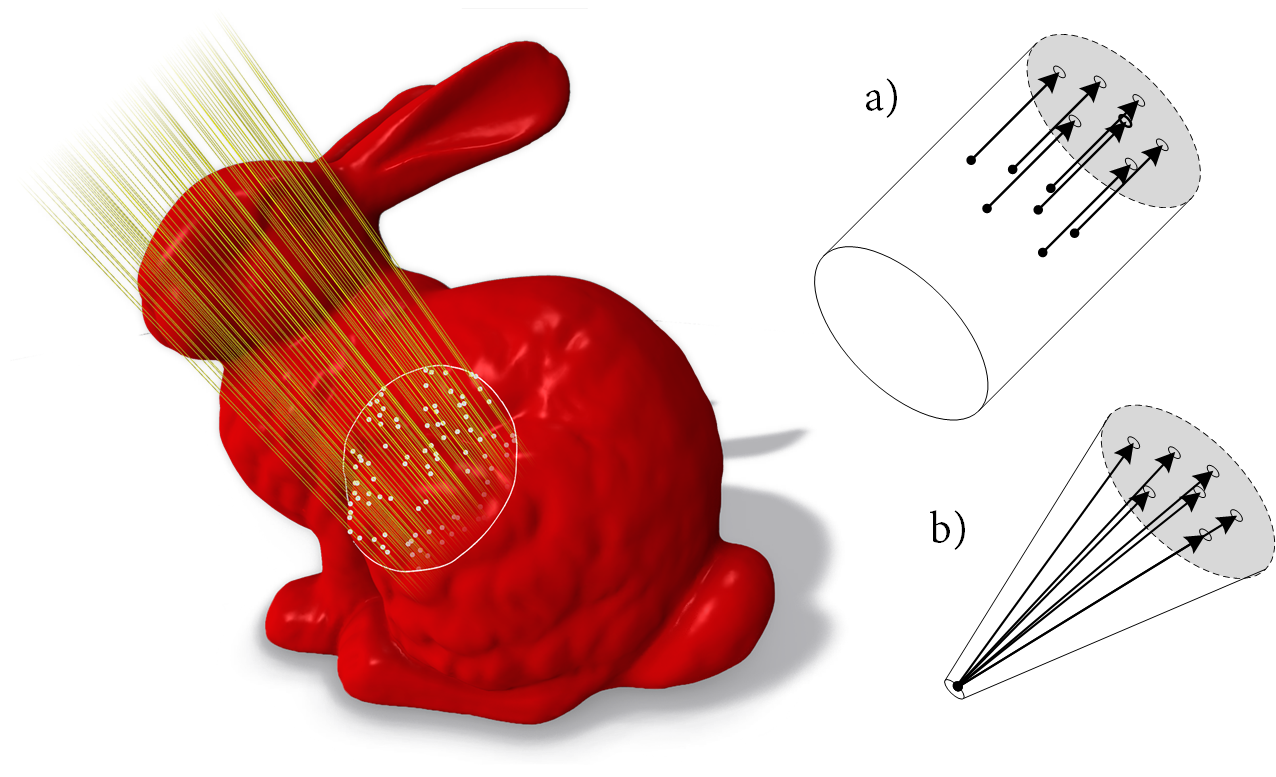
\includegraphics[width=.8\linewidth]{figs/lidar_simulation/ray_section.png}
	\caption{Collimated rays from the same pulse impacting on the Bunny model. The right side shows the scheme of a) collimated rays and b) diverging rays.}
	\label{fig:pulse_radius_insight}
\end{figure}

Regarding TLS simulations, the sphere discretization depends on the vertical and horizontal resolution ($r_x$ and $n_c$), with the first being dependent on the number of channels. Besides resolution, the surrounding environment may not be entirely covered as the horizontal field of view (FOV) can be lower than 360\textdegree. The vertical and horizontal FOV are given by $(\alpha_{\textit{start}_{xz}}, \alpha_{\textit{fov}_{xz}})$ and $(\alpha_{\textit{fov}_{y}}, \alpha_{\textit{fov}_{y}})$, with $\alpha_{o}$ being the starting angle. Therefore, the horizontal FOV covers $[\alpha_{\textit{start}_{xz}} - \frac{\alpha_{\textit{fov}_{xz}}}{2}, \alpha_{\textit{start}_{xz}} + \frac{\alpha_{\textit{start}_{xz}}}{2}]$, whereas the spacing of channels is $d_c$ (by default, it is almost zero, $\epsilon \gets 1^-16$). However, this perfect subdivision of the 3D space leads to grid-like renderings (Moiré effect) of LiDAR point clouds, which can be interpreted as an artefact. Instead, this unwanted visual effect can be avoided by jittering \cite{akenine-moller_real-time_2018} the emitted rays, thus leading to an imperfect result. Furthermore, it enables emulating beam jittering and minor inaccuracies as a result of the limited sensor accuracy \cite{mcmanamon_lidar_2019}. The random jittering uses a uniform random distribution in $[-1, 1]$ to obtain the values of the vector dispersion, $\hat{\delta}_{\textit{noise}}$, and the jittering magnitude, $\alpha_{\textit{noise}}$.

\begin{figure}[ht]
	\centering
	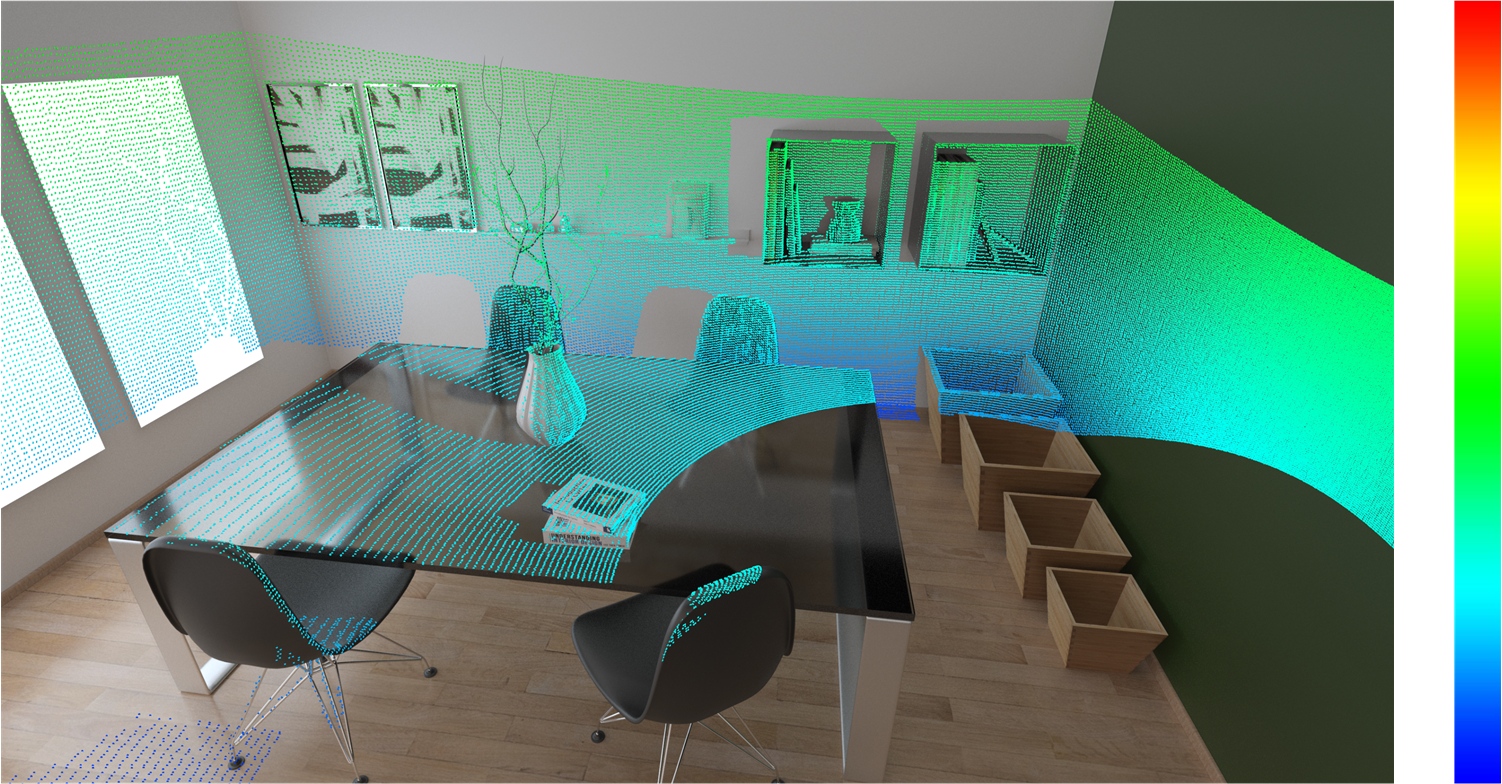
\includegraphics[width=\linewidth]{figs/lidar_simulation/tls_first_approach.png}
	\caption{Terrestrial scan with a relatively low number of spatial subdivisions, where colours vary according to the height.}
	\label{fig:tls_first_approach}
\end{figure}

Equation \ref{eq:ray_target_tls} shows the scattering direction of a beam emitted from the TLS's emitter (Equation \ref{eq:ray_origin_tls}). Horizontal lines ($\alpha_{x}$) allow calculating the position $\Theta$ on the surface of a unit sphere with $y \gets 0$, whereas the vertical lines ($\alpha_{y}$) determine the elevation of such point. Also note that $s_{d}$ and $\hat{\delta}_{xyc}$ are defined as orthogonal vectors from Equation \ref{eq:sphere_point_tls}. $r(u)$ shows the ray equation expressed through its origin, $r_{o}$, and target point, $r_{t}$. 
\begin{align*}
    &r_{o} = p + \left[0, \frac{-d_{c}\left(n_{c} - 1\right)}{2} + c d_{c}, 0\right]^\intercal 
    \numberthis \label{eq:ray_origin_tls}\\
    &r_{t} = r_{o} + \Omega_{1}\left(\hat{\delta}_{\textit{noise}}\begin{bmatrix}\lambda_{x} \\ \lambda_{y} \\ \lambda_{z} \end{bmatrix}, \alpha_{\textit{noise}}\lambda_{\alpha}\right) \Omega_{2}\left(\hat{\delta}_{xyc}, \alpha_{y}\right) \Theta
    \numberthis \label{eq:ray_target_tls}\\[.4em]
    &r(u) = r_o + u\hat{\left(r_{t} - r_{o}\right)}
    \numberthis \label{eq:ray_equation_tls}
\end{align*}
where intermediate results are calculated as follows:
\begin{align*}
    \Theta &= \left[\cos{\alpha_{x}} 0 -\sin{\alpha_{x}}\right]^\intercal 
    \numberthis \label{eq:sphere_point_tls}\\
    \hat{\delta}_{xyc} &= \left[s_{d_{z}} 0 -s_{d_{x}}\right]^\intercal
    \numberthis \label{eq:sphere_angle_tls}\\
    \alpha_{x} &= \alpha_{\textit{start}_{x}} + \alpha_{\textit{fov}_{x}}\left(\frac{x}{r_{x}} + \frac{y}{ r_{x}r_{y}} - \frac{1}{2}\right)
    \numberthis \label{eq:horizontal_angle_tls}\\
    \alpha_{y} &= \alpha_{\textit{start}_{y}} + y\left(\frac{r_{y}\alpha_{\textit{fov}_{y}} + \alpha_{\textit{fov}_{y}}}{{r_{y}}^2}\right)
    \numberthis \label{eq:vertical_angle_tls}
\end{align*}
provided that $\Omega$ represents a rotation matrix defined by a rotation axis and scalar angle, whereas $\lambda_{x}$, $\lambda_{y}$, $\lambda_{z}$ and $\lambda_{a}$ are random values generated through a random uniform distribution. $x$, $y$ and $c$ represent iterative values so that $0 \leq x < r_{x}$, $0 \leq y < r_{y}$ and $0 \leq c < n_{c}$. $\alpha_{x}$ and $\alpha_{y}$ are horizontal and vertical angles, respectively. Accordingly, $0 \leq \alpha_{x} \leq 2\pi$ and $\frac{-\pi}{2} < \alpha_{y} < \frac{\pi}{2}$. 

Furthermore, sensors such as the Pandar64 do not have uniform resolution along the vertical axis \cite{hesai_pandaset_2021}. To cope with this kind of sensors, several intervals can be expressed through the start and limit angle.  

Despite ray generation being straightforward for TLS, the latency increases significantly with high-resolution scans and long surveys. Thus, sequential generation is replaced by a massively parallel approach where individual rays are handled by different GPU threads. The main drawback of GPU is that OpenGL's compute shaders lack noise functions to build jittered rays. Some pseudo-random generators are frequently used in GLSL, though noise ought to be uniformly distributed. This was solved by building a large buffer with uniform random values in the CPU, which is later used by GPU threads to randomize LiDAR processes. Another challenge arises from the limited GPU memory since SSBOs expand to a few gigabytes at most, regardless of the GPU capacity. Therefore, the ray generation is split into several iterations that overwrite a single SSBO on which rays are stored, with each iteration being followed by the collision solver. Otherwise, CPU and GPU transfers would be larger to avoid surpassing the maximum capacity. The maximum number of allocatable rays in a single buffer is computed from the maximum capacity (queried from OpenGL), the size of a single ray and the number of rays within a pulse, $n_r$, as shown in Equation \ref{eq:max_rays_ssbo}. Note that pulse rays cannot be separated into several stages since they behave synchronously.
\begin{equation}
    \label{eq:max_rays_ssbo}   
    \textit{n}_{\textit{g}} = n_r\lfloor{\frac{\mathtt{\tiny{glGetIntegerv(GL\_MAX\_SHADER\_STORAGE\_BLOCK\_SIZE)}}}{n_r \cdot \tiny{\mathtt{sizeof(Ray)}}}\rfloor}
\end{equation}

\renewcommand{\arraystretch}{1.2}
\begin{table*}
    \caption{Configuration parameters for generating rays from an ALS. Again, angles are expressed in radians.}
    \label{table:als_parameters}
    \centering
    \begin{tabular}{ll}
    \toprule
    \textbf{Parameter} & \textbf{Description} \\
    \midrule
    Platform altitude ($h_{l}$) & Average elevation of the mobile platform during the scan.\\
    Field of view ($\alpha$) & Aperture of LiDAR sensor. \\
    Speed of the airborne platform ($s_{p}$) & Pace of the mobile platform in \si{\meter/\second}. \\
    The number of scans ($s_{l}$) & Number of scan lines per second. \\
    The number of pulses ($p_{l}$) & Number of pulses per second. \\
    Coordinates noise ($\delta_{\textit{noise}}$) & Magnitude of the random distortion applied to the ray's target.\\
    Altitude noise ($h_{\textit{noise}}$) & Magnitude of jittering in the platform altitude while scanning.\\
    Scanning pattern & Pattern used to scan the scene. \\
    Flattening of ellipses ($e_{f}$) & $y$-scale of ellipses (only for an elliptical scan pattern). \\
    \bottomrule
    \end{tabular}
\end{table*}
\renewcommand{\arraystretch}{1}

In comparison with TLS, ALS is simulated by following an aerial path. ALS pulses are emitted throughout a plane instead of a sphere, while the sensor location varies across the path. Among other features, the FOV is significantly more limited to avoid capturing atmospheric returns, though the latter is also simulated as a noise source. The jittering affects both the emitted rays and the height of the mobile platform, with a magnitude of $h_n$. Regarding resolution, it is parameterized with the number of scans and pulses per second (see Table \ref{table:als_parameters}). Instead of solely performing parallel sweeps over the environment, other patterns can be used to maximize the point cloud coverage. Figure \ref{fig:als_patterns} shows zigzag and elliptical patterns as described by Dong et al. \cite{dong_lidar_2018}. Hence, the configuration parameters of ALS are notably different from the TLS configuration (compare Table \ref{table:als_parameters} and Table \ref{table:tls_parameters}) by integrating the movement of a mobile platform where the LiDAR is coupled. Nevertheless, the flight direction of a mobile platform is not affected by scanning patterns. The sensor emitter is calculated from a linear interpolation and a parametric value, $t_i$. Therefore, $r_o$ and $r_d$ are computed according to the scanning pattern and $t_i$. The parameterization of parallel and zigzag patterns is the following:
\begin{align*}
    r_{o} &= p_{t_{i}} + 
    \begin{bmatrix} 0 \\ \lambda_{h}h_{\textit{noise}} \\ 0 \end{bmatrix} + \frac{s_{l}p_{s_{i}}}{p_{l}} \vec{d}
    \numberthis \label{eq:ray_origin_als_zigzag}\\
    r_{t} &= r_{o} - \hat{\delta}_{sp} \sin{\beta} +
    \begin{bmatrix}0 \\ -\cos{\beta}\\ 0 \end{bmatrix} + \delta_{noise}
    \begin{bmatrix}\lambda_{x} \\ \lambda_{y}\\ \lambda_{z} \end{bmatrix}
    \numberthis \label{eq:ray_target_als_zigzag}
\end{align*}
where the rotation angle $\beta$ and the vector $\hat{\delta}_{sp}$ are calculated as follows:
\begin{align*}
    \beta &= \textit{z}_{s}\alpha \left(\frac{p_{s_{i}} s_{l}}{p_{l}} - \frac{1}{2}\right)
    \numberthis \label{eq:beta_als_zigzag}\\[0.4em]
    \delta_{sp} &= \left[-\vec{d}_{z}, 0, \vec{d}_{x}\right]^\intercal
    \numberthis \label{eq:rotation_axis_als_zigzag}
\end{align*}
given that $p_{s_{i}}$ is the index of a pulse within the $\textit{i-th}$ scene sweep, $\vec{d}$ is the vehicle direction, $\delta$ is a random value from an uniform distribution and $s$ is an iterative value with $0 \leq s < n_{\textit{scans}}$. Also, $\textit{z}_{s} \in \{-1, 0, 1\}$ enables omitting workflow branching for parallel scanning sessions with $\textit{z}_{s} \gets 0$, whereas -1 and 1 are used for odd and even iterations during a $\textit{zigzag}$ scanning. 

The elliptical pattern changes the ray instancing phase since scans are depicted as an ellipse, which may be more or less flattened according to a factor of $e_{f}$ (Equation \ref{eq:ray_target_als_elliptical}). Accordingly, $\beta$ defines a circumference flattened in the $x$-axis and centred in $p_{t_{i}}$. 
\begin{align*}
    %r_{o} &= p_{t_{i}} + \begin{bmatrix}0 \\ \lambda_{h}h_{noise} \\ 0 \end{bmatrix} + \frac{s_{l}p_{s_{i}}}{p_{l}} \vec{d}
    %\numberthis \label{eq:RayOriginALSElliptical}\\
    r_{t} &= r_{o} + 
    \begin{bmatrix}e_{f} e_{r} \sin{\beta}\\ -h_{r}\\ e_{r} \cos{\beta}\end{bmatrix} + \delta_{noise}
    \begin{bmatrix}\lambda_{x} \\ \lambda_{y}\\ \lambda_{z} \end{bmatrix}
    \numberthis \label{eq:ray_target_als_elliptical}
\end{align*}
where the rotation angle, $\beta$, and the ellipse radius, $e_{r}$, are calculated in Equations \ref{eq:beta_als_elliptical} and \ref{eq:radius_als_elliptical}.
\begin{align*}
    \beta &= \frac{2 p_{s_{i}} \pi \frac{\textit{aabb}_{x}}{s_{p} s_{l}}}{\frac{\textit{aabb}_{x}}{s_{p} p_{l}}} = \frac{2 p_{s_{i}} \pi p_{l}}{s_{l}} 
    \numberthis \label{eq:beta_als_elliptical}\\[0.4em]
    e_{r} &= h_{r} \tan{\frac{\alpha}{2}}  
    \numberthis \label{eq:radius_als_elliptical}
\end{align*}
Intuitively, $e_{r}$ is computed through the tangent of $\frac{\alpha}{2}$ for any height $h_{r}$. We can simplify this whether we assume $h_{r} \gets 1$, as the ray target is correctly positioned within the environment by considering $r_{d_{y}} \gets -h_{r}$. On the other hand, $i$ is defined as the index of each incremental step and therefore is related to the parametric value $t_{i}$.

\begin{figure}
    \centering
    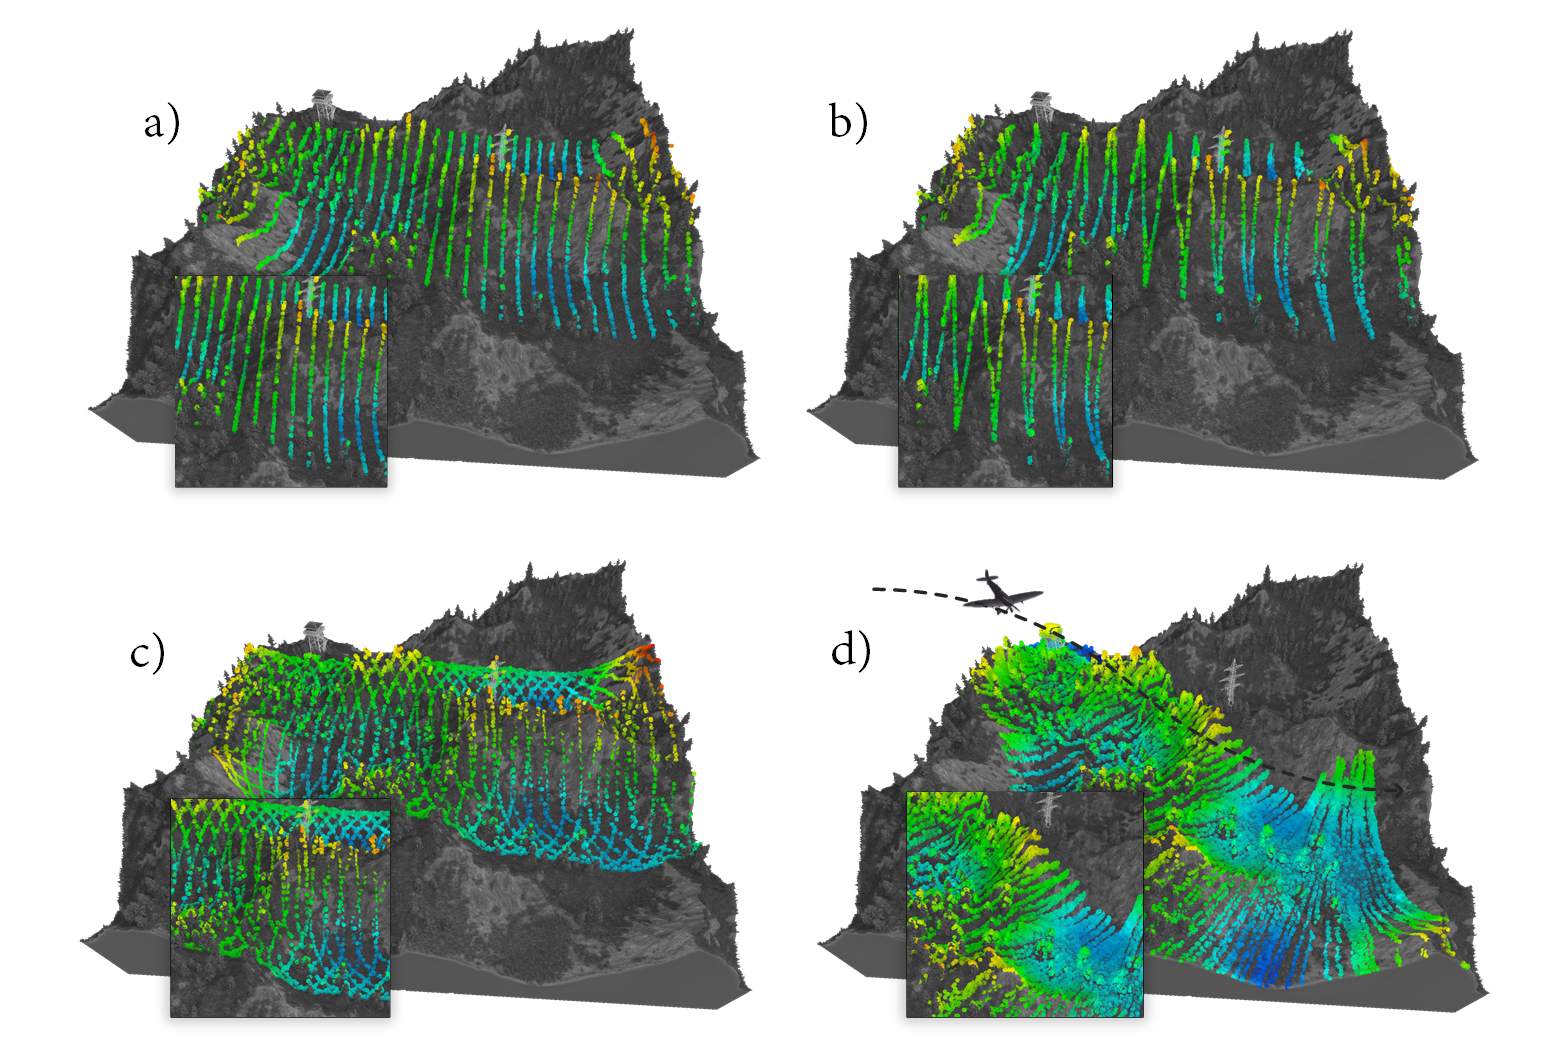
\includegraphics[width=\linewidth]{figs/lidar_simulation/als_patterns.png}
	\caption{Multiple airborne scans following these patterns: a) parallel, b) zigzag, c) elliptical and d) custom path defined by the user. }
	\label{fig:als_patterns}
\end{figure}

Scenarios can be scanned with ALS following parallel routes along the X or Z axis. Platform rotations to change its $\textit{forward}$ direction are not simulated these waypoints are typically recommended to be discarded. For instance, SpatialExplorer\textregistered software for processing LiDAR point clouds allows discarding parts of the followed path for this reason. Whether the path is computer-generated, the translation of the mobile platform follows sparse parallel lines along X-axis. The distance between these lines is calculated considering the dimensions of the environment as well as the field of view of the sensor (Equation \ref{eq:num_aerial_sweeps}), in order to extensively survey the scene. Otherwise, the path can be defined using a canvas in the Graphical User Interface (GUI). Nevertheless, user-defined paths are stored in every frame and thus collect a large number of very close and noisy points. This shortcoming is tackled by simplifying the path with the Douglas-Pecker algorithm \cite{douglas_algorithms_1973}: the path remains similar, whereas the number of points notably decreases. Then, the path points are used as control points in a Catmull-Rom spline curve that is later sampled in the scanning. Either computer-generated or defined by users, the paths are sampled in the CPU and transferred to the GPU to make this routine simpler in GPU processing. 
\begin{equation}
    n_{\textit{steps}} = \lceil{\frac{p_{\textit{min}_z}}{2(h_{l} - p_{\textit{min}_y})\tan(\frac{\alpha}{2})}\rceil}
    \numberthis \label{eq:num_aerial_sweeps}
\end{equation}
where $p_{\textit{min}}$ is the minimum of the scene's AABB.

Finally, the ray emission in ALS changes considerably; firstly, diverging laser beams within a pulse were simulated instead of conventional collimated/parallel beams, as proposed by Zohdi \cite{zohdi_rapid_2020}. Given a radius $r$ defined at a distance $d \gets 1$, several rays are scattered using the result of Equation \ref{eq:ray_target_diverging}. For each ray, an orthonormal basis is constructed ($\hat{u}, \hat{v}, \hat{r}_{d}$) using the ray direction, $r_{d}$, as well as an up vector, $\hat{\textit{up}}$, expressed as $\left[0, 1, 0\right]^\intercal$ for a TLS LiDAR. Accordingly, $\hat{u}, \hat{v}$ correspond to $x$ and $y$-axis for a ray basis, and therefore, scaling both vectors by a random factor $\delta_{r} \in [-r, r]$ and adding them to ray target ($r_{t}$) leads to a diverging beam. For that purpose, the point calculated in Equation \ref{eq:ray_target_diverging}, $p_{d_{i}}$, satisfies $D(p_{d_{i}}, r_{t}) < r$, provided that $i$ is bounded by the number of discrete rays, $n_{p}$, and $D$ is a function measuring the distance between two points. Consequently, the LiDAR is better simulated with larger values of $n_{p}$, despite requiring larger memory allocation.
\begin{gather}
    \label{eq:ray_target_diverging}
    \begin{aligned}
        p_{d_{i}} &= r_{o} + \hat{r}_{d} + \hat{u}\delta_{r} + \hat{v}\delta_{r} = r_{t} + \hat{u}\delta_{r} + \hat{v}\delta_{r}\\
        \vec{u} &= \hat{\textit{up}} \times \hat{n}\\
        \vec{v} &= \hat{n} \times \hat{u}
    \end{aligned}
\end{gather}

\subsection{Collision solver}

\renewcommand{\arraystretch}{1.2}
\begin{table*}
    \small
    \caption{Generic configuration attributes used during any LiDAR simulation. Thus, these parameters have not been previously listed as ALS or TLS-related properties.  }
    \label{table:lidar_workflow_parameters}
    \begin{tabular}{ll}
    \toprule
    \textbf{Parameter} & \textbf{Description}\\
    \midrule
    Wavelength ($\lambda$) & 532 \si{\nano\meter} for bathymetric scans, 1064 \si{\nano\meter} otherwise.\\
    Pulse radius ($r$) & Radius at a distance of $t = 1$ following the ray parametric equation. \\
    Rays per pulse ($n_{p}$) & Accuracy of pulse discretization. \\
    Energy ($\bar{I}$) & Energy linked to a ray pulse, given in \si{\watt}. \\
    Sensor diameter ($p_{l}$) & Diameter of the LiDAR's receiver component (\si{\meter}). \\
    The maximum number of returns ($n_{r}$) & Number of maximum returns for a single pulse. \\
    Maximum range ($R$) & Maximum range covered by pulses.\\
    Noise boundary of $R$ ($R_{\delta_{\textit{min}}}, R_{\delta_{\textit{max}}}$) & Noisy boundary to avoid abrupt clamping at a distance of $R$.\\
    Terrain-induced error ($e_{\textit{terrain}}$) & Boolean value indicating if terrain errors are simulated. \\
    Shiny surface error ($e_{\textit{glossy}}$) & Boolean value indicating if highly reflective surfaces present some distortions. \\
    Outlier threshold ($t_{\textit{outlier}}$) & Probability of generating outlier points. \\
    Outlier range ($t_{\textit{min}}, t_{\textit{max}}$) & Dispersion of outliers. \\
    Atmospheric attenuation ($a_{\textit{atm}}$) & Atmospheric attenuation factor (see Equation \ref{eq:lidar_equation}). \\
    System transmission ($n_{\textit{sys}}$) & System transmission factor (see Equation \ref{eq:lidar_equation}). \\
    \bottomrule
    \end{tabular}
    \libertineNormal
\end{table*}
\renewcommand{\arraystretch}{1}

The generated TLS and ALS rays interact with surfaces to build dense semantic point clouds from a virtual LiDAR sensor. Rays behave following a set of synchronous stages shown in Figure \ref{fig:lidar_workflow}, regardless of the scanning platform. Particularities on TLS and ALS can be implemented through shader subroutines rather than different pipelines. The GPU-based stages manipulate and share the SSBO buffers to avoid CPU data transfers, with an explicit barrier avoiding different stages to work asynchronously. Stages involving randomness use buffers generated with a custom random distribution and accessed with an offset according to the thread index. Quasi-Monte-Carlo (QMC) samplers, such as the Halton generator, and the C++ built-in uniform random distribution are here used, though others can be integrated. The number of rays processed during a single iteration is a multiple of $n_{p}$.

The stages depicted in Figure \ref{fig:lidar_workflow} are following described:

\subsubsection{Ray initialization}

Initially, rays carry out a starting energy value which later affects the measured intensity. The returned ID is also set to zero. Their carried energy is updated to $\bar{I}_{i} = \bar{I} / n_{p}$, with $\bar{I}$ being the energy of a single pulse in watts (\si{\watt}). The return number is set to zero and the refractive index is initially one (air substance). 

\begin{marginfigure}[.0cm]
	\centering
	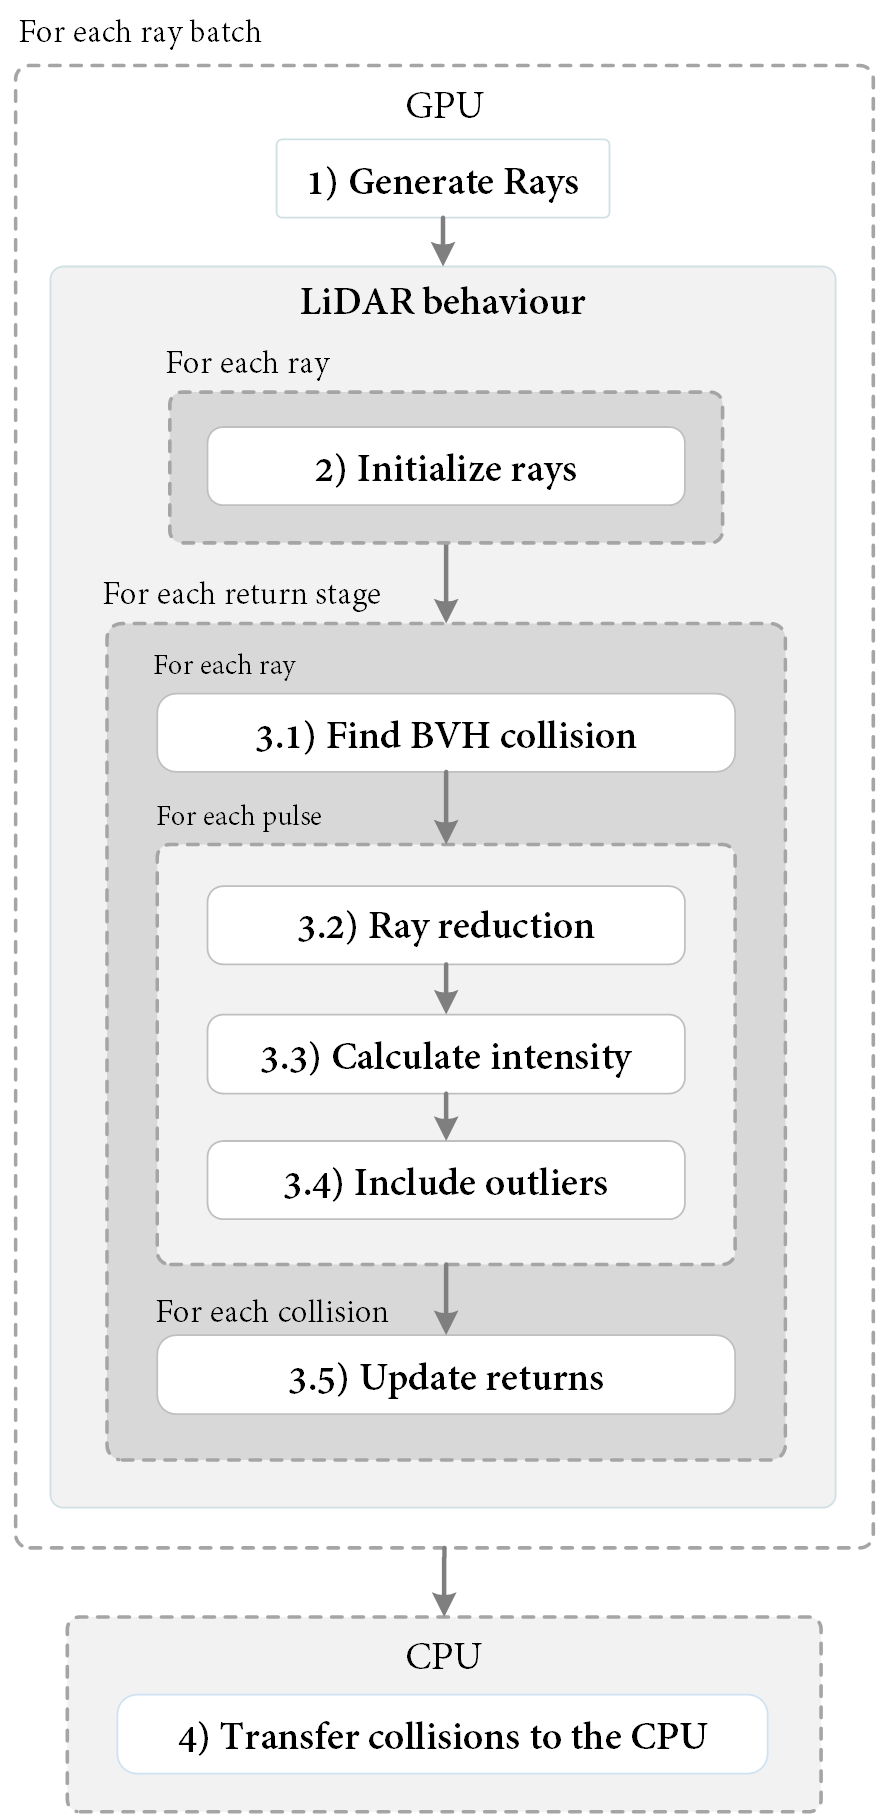
\includegraphics[width=\linewidth]{figs/lidar_simulation/lidar_overview.png}
	\caption{Summary of the LiDAR workflow as implemented in the CPU and GPU. CPU processing is minimized during this pipeline to avoid delays from data transfers.}
	\label{fig:lidar_workflow}
\end{marginfigure}
\textbf{Find collision in the BVH}. Each ray finds the nearest intersected surface and polygon if it exists. Solving this stage requires the scene BVH as well as computing ray-AABB and ray-triangle intersections. This stage is based on the time-of-flight principle, thus allowing us to estimate the object distance by timing the travel distance of the laser beam, whose velocity is known. If a collision is identified for the ray $r_{i}$, the indices of the collided face and surface are stored in a collision buffer. 

\subsubsection{Ray reduction}

Next, rays act as a single pulse and therefore, the number of shader calls are $p$ instead of $n_{p}p$. This stage is relevant for simulating multiple returns in environments such as forests. Hence, rays which are not terminated early penetrate high and low vegetation, allowing them to acquire ground features not visible under normal conditions. Although multiple collisions can be detected, the nearest one is utilized in later stages. Thus, threads that impacted on a such surface or did not collide are terminated, whereas the rest continue their path. Several collisions are considered to impact the same chunk of a surface if multiple criteria are met. 
\marginnote[5.0cm]{
    Measuring the distance solely with $2dr + \epsilon$ leads to omitting those collisions whose $\hat{n} \cdot \hat{r}_{d}$ highly differs from 1. Consequently, the maximum distance is corrected as shown in Equation \ref{eq:pulse_radius_slope_distance}.
}
\begin{itemize}
    \item Collisions fall in the same triangle. This assumption cannot be applied to objects, since triangle meshes represented by several not-enclosed surfaces, such as leaves, lead to ultimately missing some returns.
    \item Distance among collisions is smaller than $2 - \left|\hat{n} \hat{r}_{d}\right|$ to take into account the surface normal vector. Accordingly, it is notated as shown in Equation \ref{eq:pulse_radius_slope_distance}, given that $d$ is the distance from the collision to the LiDAR's receiver component, $r$ is the pulse radius and $\hat{n}$ is the surface normal.
    \begin{equation}
        \label{eq:pulse_radius_slope_distance}
        d_{\textit{max}} = 2dr \cdot (2 - \left|\hat{n} \cdot \hat{r}_{d}\right|)
    \end{equation}
    \item Collided triangles are adjacent and therefore they share at least two vertices. Given the limited radius of a single pulse, checks of one-level depth have been sufficient for detecting equal collisions.
\end{itemize}

The ray attributes are changed based on the conclusions extracted from here. Those that collided with a surface, despite not being the closest one, follow their path, in contrast to those that did not collide or caused the current return. Consequently, each laser pulse may iteratively find several returns, and each detected collision has its own return number that is later completed with the number of collisions returned per pulse at the end of this stage. 
  
Nevertheless, some collisions may be discarded if the maximum range is surpassed. To provide a smooth boundary, it is randomized with a configured dispersion. Surface slope also influences the distortion of returned collisions, both on vertical and horizontal axes \cite{deems_lidar_2013}. The magnitude of such errors depends on the distance to the sensor, thus being significantly higher in aerial scans. Previous research has helped in selecting an appropriate value for this distortion \cite{hodgson_accuracy_2004}. Finally, a significant number of return errors are derived from shiny surfaces with high reflectance. This is modelled by simulating the 'time-walk' effect, on which beams are reflected multiple times, thus increasing the time-of-flight and the measured distance. This even leads to losing some of these returns. 

\textbf{Maximum range of ToF measurements}. Given the maximum distance, $R_{\textit{max}}$, and a noisy boundary, defined through $R_{\delta_{\textit{min}}}$ and $R_{\delta_{\textit{max}}}$, with $R_{\delta_{\textit{min}}} \leq 0 \leq R_{\delta_{\textit{max}}}$, a point is discarded if the distance to the sensor, $d$, satisfies Equation \ref{eq:noisy_boundary}.
\begin{equation}
    \label{eq:noisy_boundary}
    d > R + \delta (R_{\delta_{\textit{max}}} - R_{\delta_{\textit{min}}}) + R_{\delta_{\textit{min}}}
\end{equation}
provided that $\delta$ is a random value retrieved from a uniform random distribution ranging from 0 to 1. Here, $R_{\delta_{\textit{min}}}$ and $R_{\delta_{\textit{max}}}$ are expressed as values relative to $R$ instead of absolute range values. For instance, $R_{\delta_{\textit{min}}} \gets -1 \si{\meter}$ and $R_{\delta_{\textit{max}}} \gets 1 \si{\meter}$. Figure \ref{fig:tls_maximum_range} depicts wide boundaries expressed through $R_{\delta_{\textit{min}}}$ and $R_{\delta_{\textit{max}}}$ for terrestrial technology.

\begin{figure}[ht]
	\centering
	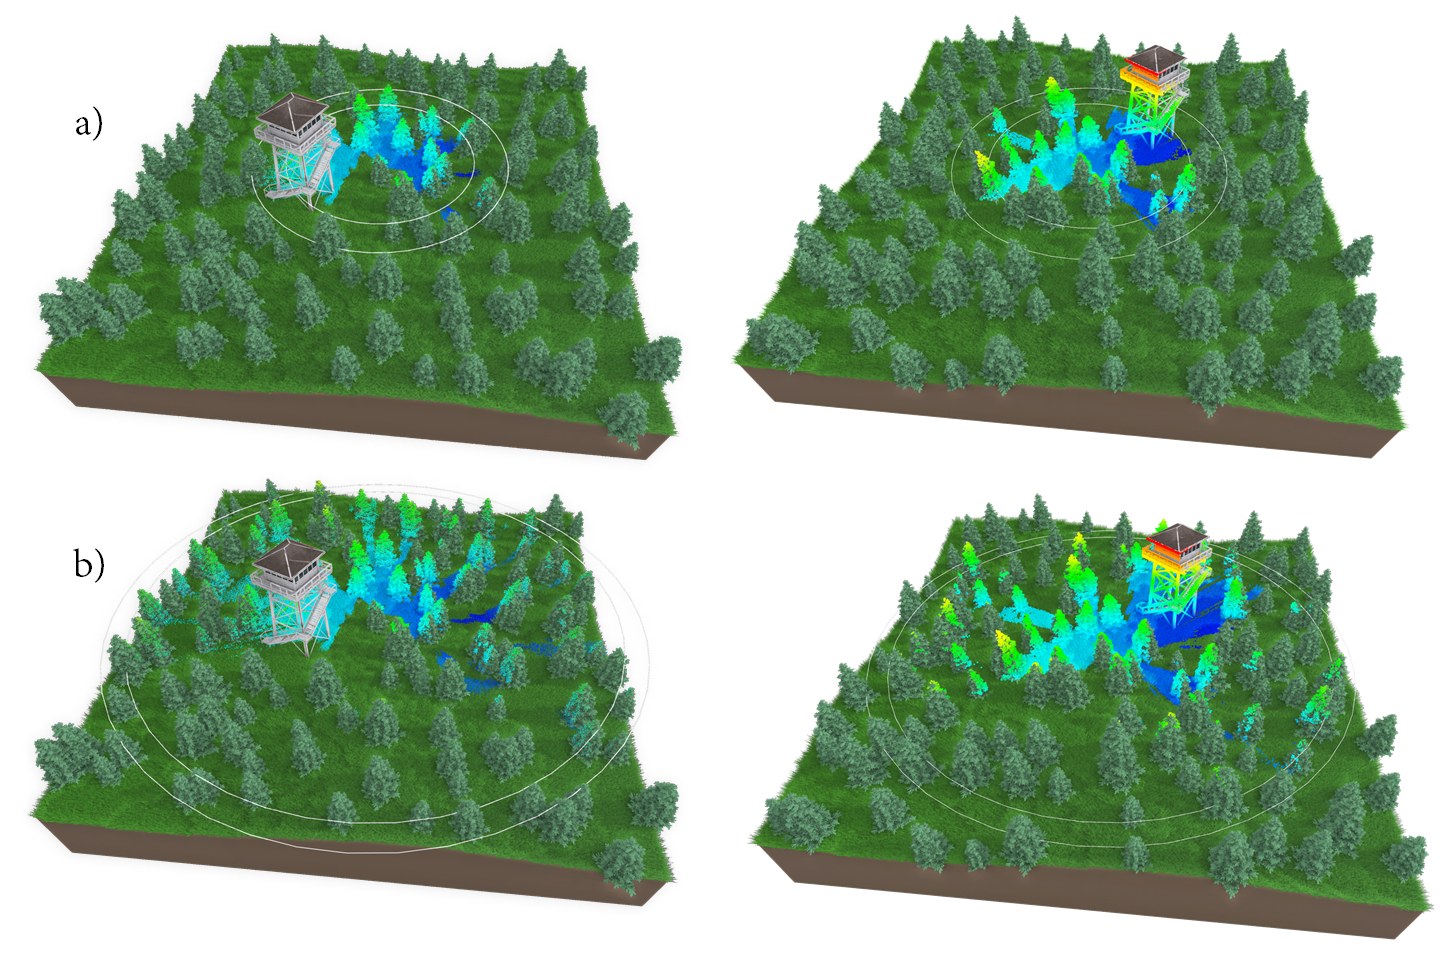
\includegraphics[width=\linewidth]{figs/lidar_simulation/tls_maximum_range.png}
	\caption{Two different scenes, a) and b), scanned with different boundaries.}
	\label{fig:tls_maximum_range}
\end{figure}

\textbf{'Time-walk' effect}. This effect is simulated by translating returns according to three factors: the distance to the sensor's receiver and the indices that identify the surface and collision. Hence, index-related factors are linked to two random values ($\delta_{\textit{object}}$, $\delta_{\textit{return}}$). $\delta_{\textit{surface}}$ helps to preserve the surface shape and is the same for every return over the same object, whereas $\delta_{\textit{return}}$ introduces some minor changes to every different return. Still, the magnitude of this error is mainly driven by the distance factor (Equation \ref{eq:shiny_surface_error}).
\begin{equation}
    \label{eq:shiny_surface_error}
    e_{\textit{glossy}} \cdot (d \cdot \hat{r}_{d} k_{\textit{distance}} + \hat{r}_{d}(\delta_{\textit{surface}}k_{\textit{surface}} + \delta_{\textit{collision}}k_{\textit{collision}})) 
\end{equation}
where $k_{\textit{distance}}$, $k_{\textit{surface}}$ and $k_{\textit{collision}}$ are constant values that control the magnitude of the equation term, $\textit{glossy}$ is a Boolean value that determines if such error is applied, and $d$ is the distance from the sensor to a collision. Figure \ref{fig:shiny_surface_error} shows the translation applied to highly reflective objects if the LiDAR's eye is close to the affected surfaces.

\begin{figure}
	\centering
	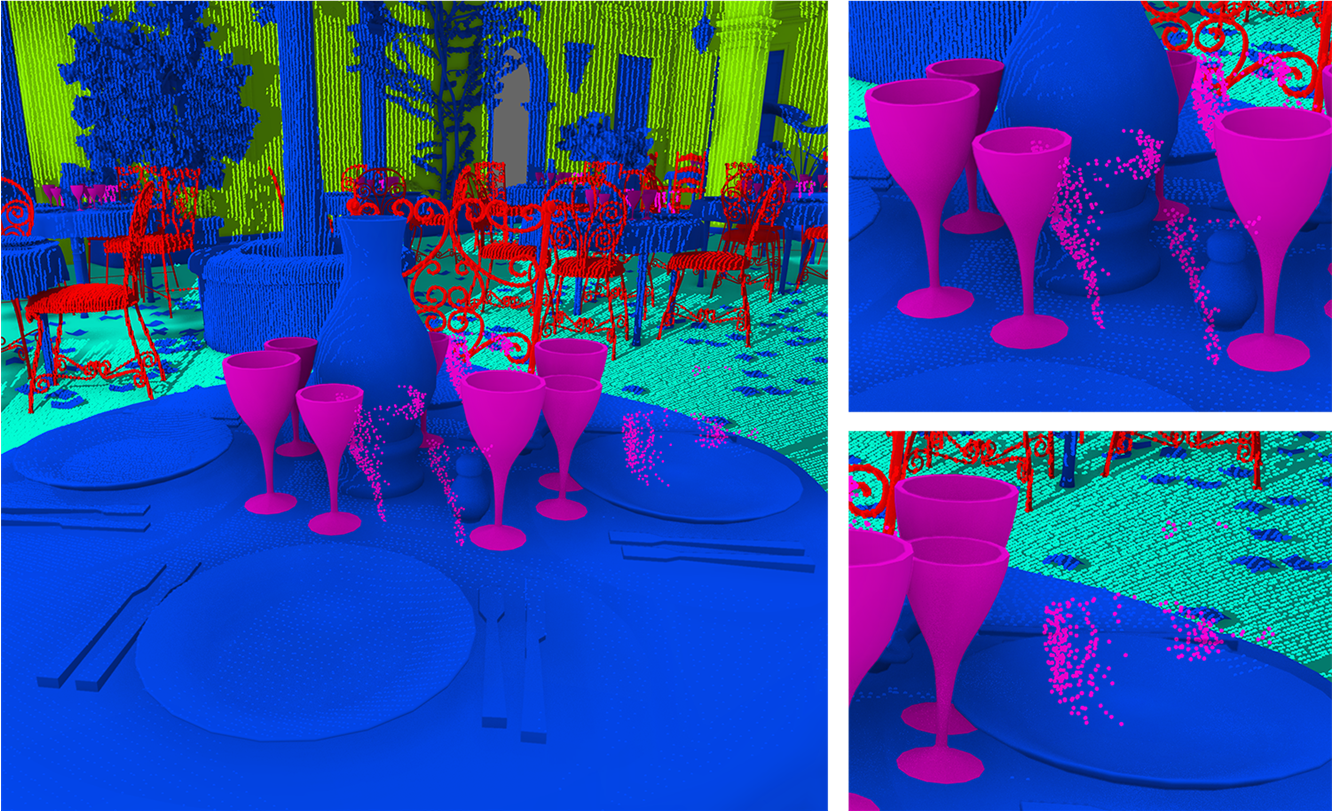
\includegraphics[width=.8\linewidth]{figs/lidar_simulation/glossy_time_walk.png}
	\caption{'Time-walk' effect simulated on glass surfaces rendered according to their semantic labels. }
	\label{fig:shiny_surface_error}
\end{figure}

Finally, points are also distorted in forestry areas according to the airborne flight altitude (vertical error) and the slope (horizontal error). The former is calculated as $\frac{h}{10^3}$ \si{\meter}, with $h$ being the airborne platform altitude \cite{hodgson_accuracy_2004}. The altitude-based error depends on the surface slope and flight altitude \cite{baltsavias_comparison_1999} (see Equation \ref{eq:soil_induced_error}).
\begin{gather}
    \label{eq:soil_induced_error}
    \begin{aligned}
        e_{\textit{terrain}} \cdot (&\delta_{h} k_{\textit{height}_{h}} h 
        \left[\delta_{x}, 0, \delta_{z}\right]^\intercal + \delta_{v} (k_{\textit{height}_{v}} h + k_{\alpha} \alpha)
        \left[0, 1, 0\right]^\intercal)
    \end{aligned}
\end{gather}
provided that $h$ is the flight altitude and $k_{\textit{height}_{v}}$, $k_{\textit{height}_{h}}$,  $k_{\alpha}$ weight the flight altitude and slope angle for the horizontal and vertical errors. Figure \ref{fig:terrain_induced_errors} shows the outcome of this distortion. All these errors can be omitted by weighting them as zero.

\begin{figure}
    \centering
    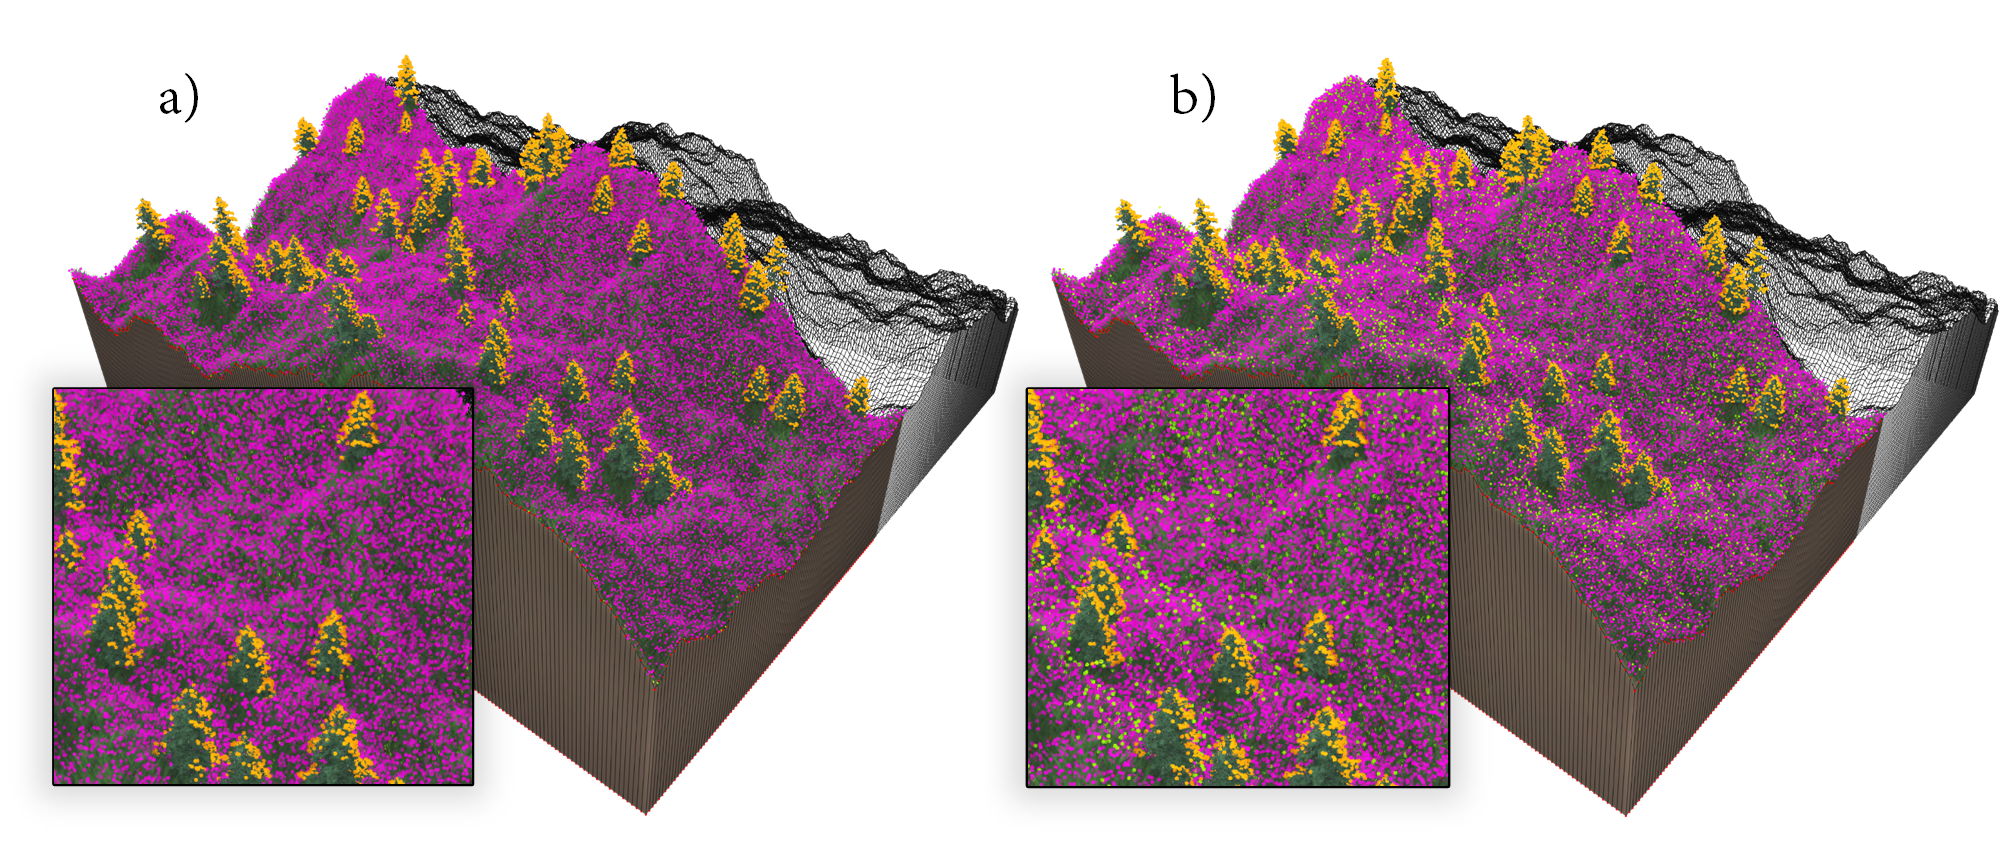
\includegraphics[width=\linewidth]{figs/lidar_simulation/terrain_induced_errors.png}
	\caption{Terrain-induced errors for a procedural environment. a) depicts an environment scanned without slope-based errors, whereas b) simulates such errors, thus making these points visible in the foreground. }
	\label{fig:terrain_induced_errors}
\end{figure}

\textbf{Bathymetric LiDAR}. This kind of sensor presents some changes with respect to the topographic LiDAR, i.e., the default one. It is able to generate collisions underwater and yet propagates causing new returns after colliding surfaces underwater. The ray's origin is always updated as $r_{o} = p + \epsilon$, though in these cases, they keep carrying the same amount of energy. The direction after colliding is computed as the refraction for the incident vector $\hat{r}_{d}$, the surface normal, $\hat{n}$, and the ratio of refractive indices, $r_{i}$. In addition, $r_{i}$ is given by the refractive index of the substance where the ray propagates, $\eta_{1}$, as well as the index of refraction from the substance of collided surface material, $\eta_{2}$. Moreover, $\eta_{2}$ depends on the wavelength of the LiDAR sensor, and therefore, the material description ought to present the refractivity over a wide spectral interval to be queried

\textbf{Return loss}. The return loss over glossy surfaces is driven by an exponential function, $g(k_{s})$, the coefficients $a, b, c, p$, a threshold $\textit{t}$ and the material's roughness, $k_s$, as shown in Equation \ref{eq:return_loss}. Hence, returns from glossy surfaces whose specular factor is above $\textit{t}$ are discarded whether the value retrieved from a random distribution is smaller than $g(k_{s})$. Accordingly, surfaces with lower reflectivity are less likely to induce errors in the incoming rays. Thus, we can define a function to partially or entirely discard water returns, as depicted in Figure \ref{fig:glossy_loss}. 
\begin{gather}
    \label{eq:return_loss}
    g(k_{s}) = \begin{aligned}
        \begin{cases}
            c + a (k_{s} + b) ^ {p} &k_{s} > \textit{t}\\
            c &k_{s} \leq \textit{t}\\
        \end{cases}
    \end{aligned}
\end{gather}
where $c$ allows introducing some randomness even for diffuse materials. However, $c$ is defined as zero by default.

\begin{figure}
	\centering
	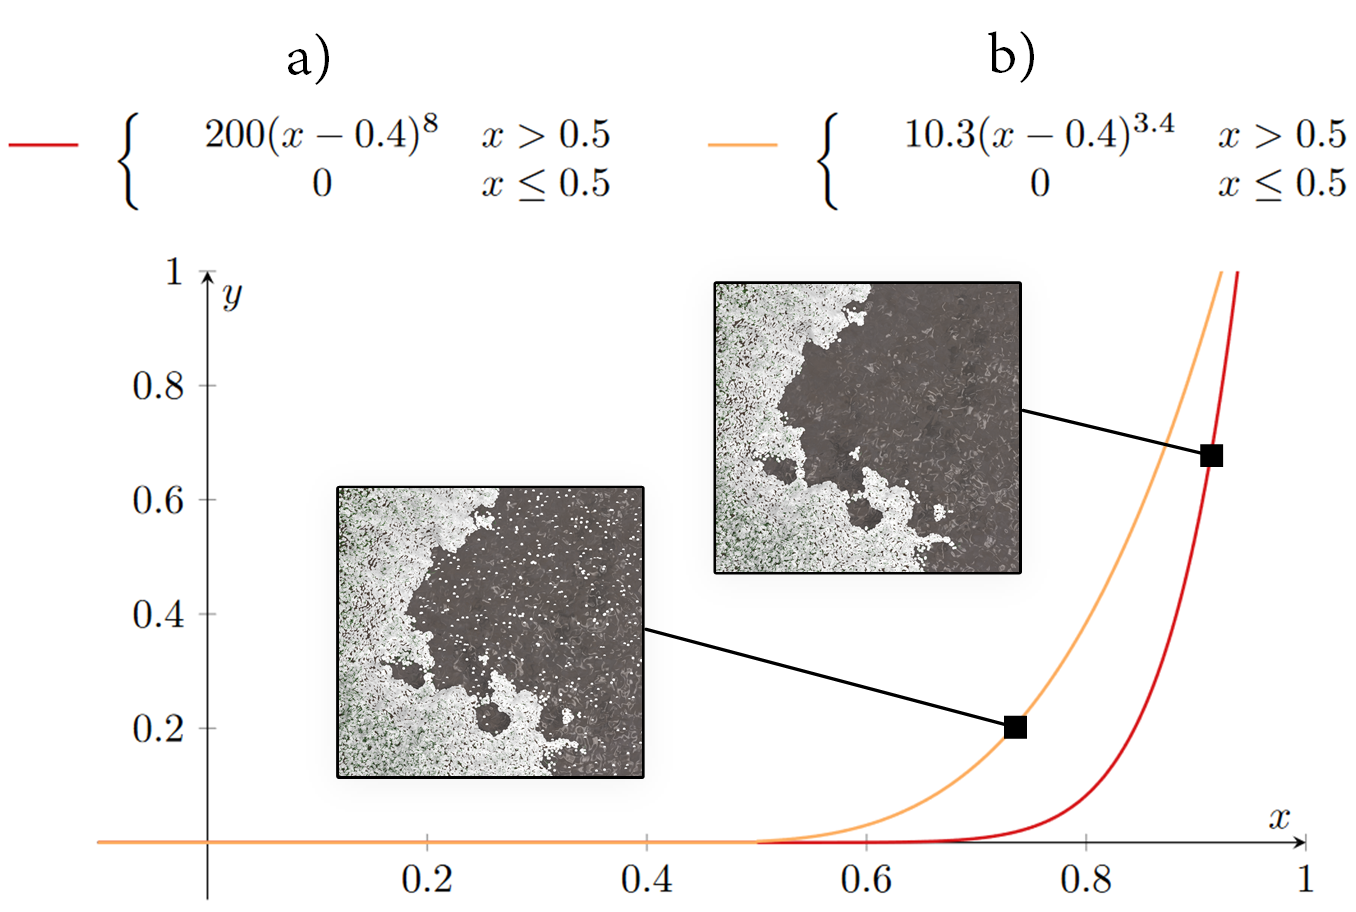
\includegraphics[width=.85\linewidth]{figs/lidar_simulation/glossy_loss.png}
	\caption{a) Loss function that slightly tolerates surfaces as glossy as water, and b) another loss function that discards every return from glossy surfaces. }
	\label{fig:glossy_loss}
\end{figure}

\subsubsection{Intensity computation}

This stage evaluates radiometric information acquired by the virtual LiDAR. It will be further explored in the later chapter, and therefore, this stage is simply aimed at providing the fundamentals of LiDAR intensity. Radiometric data is also relevant for Deep Learning applications and therefore, objects ought to be modelled accordingly. Nevertheless, unitless intensity values are influenced both by surface metadata and the LiDAR capabilities, including the operating wavelength (for instance, bathymetric LiDAR works at 532 \si{\nano\meter}). The received optical power is defined by Equation \ref{eq:lidar_equation} using the transmitted power, the reflectance of the surface and other acquisition parameters. It has been revised in the literature under multiple analogous forms \cite{hofle_correction_2007, bolkas_effect_2018, dong_lidar_2018}, despite most of them achieving an expression such as Equation \ref{eq:lidar_equation} \cite{kashani_review_2015}:
\begin{gather}
    \label{eq:lidar_equation}
    \begin{aligned}
        P_{r} &= \frac{\bar{I} D^{2}_{r} \eta_{atm} \eta_{sys} \sigma}{4 \pi d^{4} \beta^{2}_{t}}\\
        \sigma &= \frac{4\pi f_{r}(\vec{w})A_{t}}{\Omega}\\
        A_{t} &= \frac{\pi d^{2} \beta^{2}_{t}}{4}
    \end{aligned}
\end{gather}
where $\bar{I}$ is the emitted energy, $D^{2}_{r}$ is the receiver diameter (\si{\meter}), $\eta_{atm}, \eta_{sys}$ are atmospheric and system transmission factors, $f_{r}(\vec{w})$ is the target reflectance, $A_{t}$ is the target area, $d$ is the distance to receiver (\si{\meter}), $\beta$ is the transmit beam width (\si{\radian}) and $\Omega$ is the scattering solid angle (\si{\steradian}).

The scattering solid angle is computed as $A / r^{2}$, therefore it can also be expressed as $\Omega = \pi r^{2} / r^{2} = \pi$. Also, the sensor's emitter is assumed to be equivalent to its receiver. The attenuation factor $\eta_{sys}$ is a system-dependent factor that varies over time and with different systems. Hence, it is 1 by default, despite serving as a configured factor. $\eta_{atm}$ stands for a transmission factor that depends on atmospheric conditions \cite{hofle_correction_2007} and differs for horizontal and vertical propagation. Additionally, $\eta_{atm}$ is linked to the measured distance and is frequently approximated as $10^{-2da_{atm}}$, provided that $a_{atm}$ is the atmospheric attenuation factor and $d$ stands for the measured distance. With these assumptions, Equation \ref{eq:lidar_equation} is simplified as follows:
\begin{equation}
    \label{eq:lidar_equation_simplified}
    P_{r} = \frac{\bar{I} D^{2}_{r} f_{r}(\vec{w}) 10^{-2da_{atm}} \eta_{sys}}{4 d^{2}}
\end{equation}

On the other hand, the formulae for bathymetric LiDAR have a larger number of parameters interrelated as shown in Equation \ref{eq:bathymetric_lidar} \cite{narayanan_classification_2009}:
\begin{equation}
    \label{eq:bathymetric_lidar}
    P_{r} = \frac{\bar{I} f_{r}(\vec{w}) \eta F_{p} A_{r} \cos^{2}{\theta}}{\pi(\eta_{\textit{water}} H + D)^{2}} e^{-2 n_{s} \rho_{d_{\textit{water}}} D sec(\phi)}
\end{equation}
given that $\bar{I}$ is the emitted energy, $\eta$ is the system efficiency factor, $F_{p}$ is the loss due to insufficient FOV, $A_{r}$ is the area of receiver optics, $\theta$ is the angle between ray direction and nadir, $n_{w}$ is the refractive index of water (1.33), $H$ is the distance of LiDAR receiver to water, $D$ is the bottom depth underwater, $\rho_{d_{\textit{water}}}$ is the diffuse attenuation of water, $n_{s}$ is the pulse stretching factor and $\phi$ is the angle enclosed by the pulse direction and $\textit{nadir}$ vector after entering the water.

\begin{marginfigure}[.3cm]
	\centering
	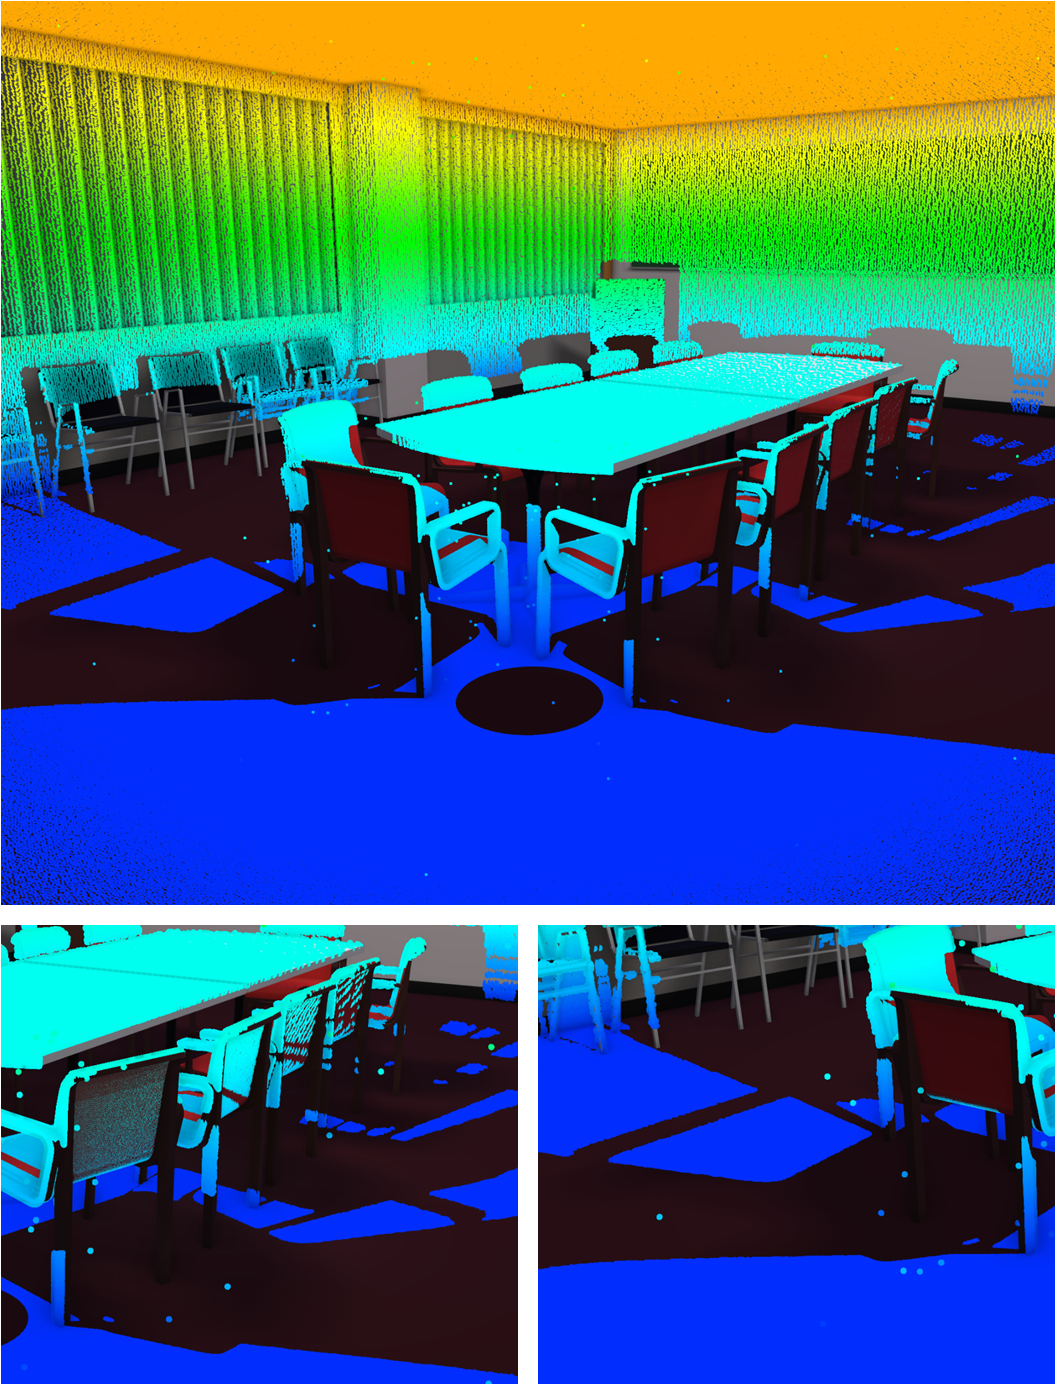
\includegraphics[width=\linewidth]{figs/lidar_simulation/outliers.png}
	\caption{Outliers in a TLS simulation, with $h \gets 0.95$.}
	\label{fig:lidar_outliers}
\end{marginfigure}

\subsubsection{Simulating outliers}

Outlier points are included to simulate errors caused by atmospheric conditions, including temperature, atmospheric pressure variations, dust or steam \cite{boehler_investigating_2018}. To this end, a variable part ($h \in [0, 1]$) of the recorded collisions is translated using the ray parametric form ($p = r_o + r_d * t$) and a random $t \in [0, 1]$ modelled with a pseudo-random generation, which is particularly relevant to determine the spatial distribution of outliers. The simulation of outliers leads to point clouds such as the one depicted in Figure \ref{fig:lidar_outliers}.

\subsubsection{Update of return attributes}

Pulses are updated once all the rays finish their path or reach the maximum number of returns. The resulting points are updated to store the overall number of collisions per pulse. The return number provides helpful information within a point cloud, though it can be further enriched by computing the factor $k_{r}$, defined as $\frac{r}{n_{r}}$, i.e., the return number divided by the overall number of returns. A higher return number more likely belongs to the soil surface, although filtering by the return number also omits ground-labelled points. However, the last collision of every pulse is returned whether we filter by $k_{r} > 1 - \epsilon$, allowing us to discard vegetation and visualize points near the ground surface. For example, archaeological explorations based on LiDAR sensors filter the last returns to find the archaeological remains through the DTM.

\begin{figure}[ht]
	\centering
	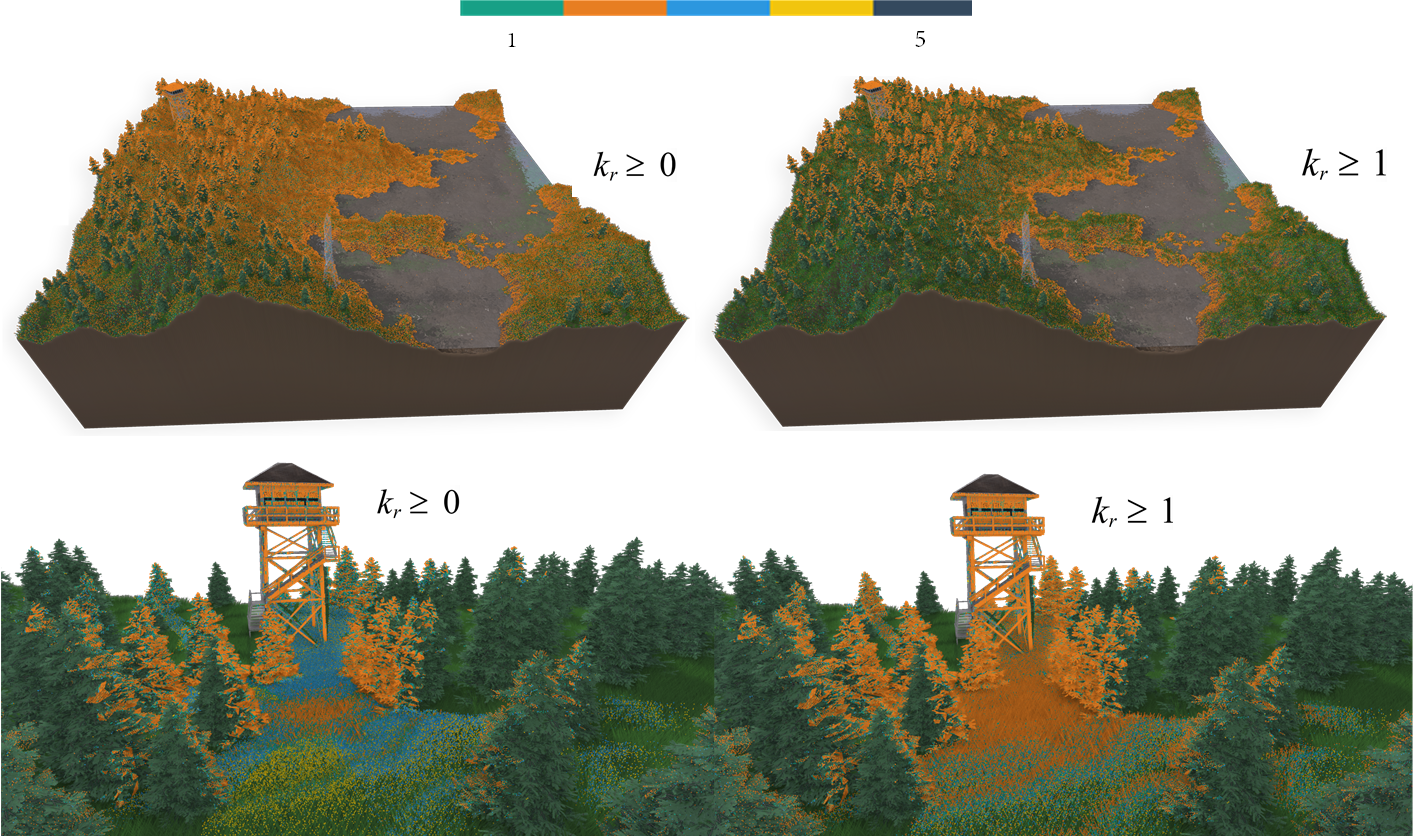
\includegraphics[width=1\linewidth]{figs/lidar_simulation/tls_multiple_returns.png}
	\caption{ALS simulation for a procedural environment. First, the complete point cloud is rendered ($k_{r} \geq 0$), whereas the second image renders only the last return of each pulse.}
	\label{fig:multiple_returns}
\end{figure}

Figure \ref{fig:multiple_returns} depicts two different point clouds filtered by means of $k_{r}$ to visualize the last return of each pulse. The forest canopy was significantly dense, thus making many pulses end their path on the vegetation, whereas low vegetation is easily avoidable. Accordingly, it shows a much less dense point cloud at ground level when $k_{r} \geq 1$, since ground points are occluded and low-vegetation collisions are filtered out. 

\section{Results and discussion}

The proposed LiDAR simulator has been tested against static and procedural scenes with high polygonal complexity (from 5M triangles to 11M). four scenes modelled by professional 3D generalists, ranging from 330k to 6M triangles. Also, it is checked through its performance by considering both response time and resulting point clouds. Other simulators in the literature focus on the behaviour of the simulation itself rather than its speedup. Thus, we compared the GPU-based approach against a sequential workflow. Finally, the described LiDAR is compared against several state-of-the-art LiDAR solutions by addressing both quantitative factors, such as their capacity to generate dense semantic datasets, and qualitative measures, such as the fidelity of the simulation with respect to real LiDAR scans. 

Measurements were performed on two different hardware configurations. Tests are carried out in a PC with Intel Core i9-9900 3.1 GHz, 48 GB RAM, RTX 2080 Ti GPU with 11 GB RAM (Turing architecture). The proposed methodology is implemented in C++ 17 along with OpenGL for rendering and ImGui for providing a Graphical User Interface. Massively parallel processes are developed in GLSL using general-purpose compute shaders. 

\subsection{LiDAR response time}

A comparison of our GPU-based method against its analogous multi-core CPU version was performed to show the efficiency of the proposed simulation. Synchronism was established among the pipeline stages to await the end of GPU calls, thus allowing us to measure the GPU latency properly. In contrast to the phase where ray collisions are computed, the response time of the first phase, i.e., ray instancing, is shared if the sensor is configured in the same manner, regardless of the input scene. Figure \ref{fig:lidar_response_time_global} summarizes the results obtained for TLS and ALS surveys, using scenes of an increasing number of polygons: Suburb (4.1M), San Miguel (4.5M), City (10.1M), Forest (11M). Multiple-return simulations were limited by five returns. These results are shown in detail in Table \ref{table:lidar_response_time}.

\begin{figure*} [ht]
	\centering
	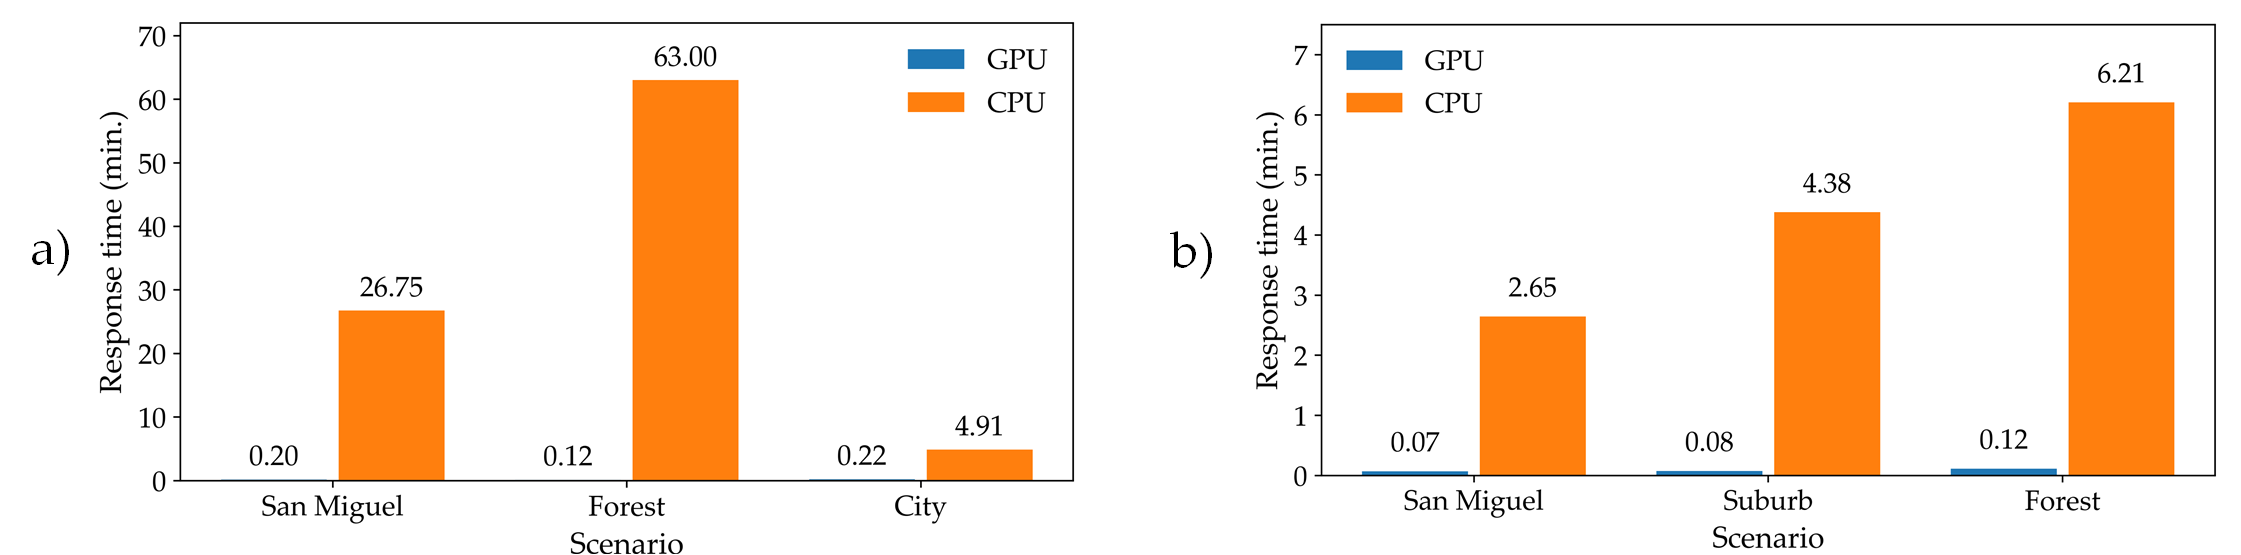
\includegraphics[width=\linewidth]{figs/lidar_simulation/response_time.png}
	\caption{Comparison of response time between the GPU and multi-core CPU approach using multiple-return a) TLS and b) ALS with $n_p \gets 10M$ and $n_r \gets 10$. }
	\label{fig:lidar_response_time_global}
\end{figure*}

\textbf{Ray build time}. TLS beams were straightforwardly computed, and thus the instancing phase shows lower latency. On the other hand, ALS beams require a larger number of parameters and computations involving angles and the followed path. The response time for 10M pulses grows linearly with respect to 5M. Despite CPU-based ray building not being as time-consuming as the LiDAR core, the speedup ranged from 90.9\% (ALS, 10M pulses) to 99.12\% (TLS, 10M pulses).

\textbf{LiDAR behaviour}. The ToF solver operates for every batch of rays, with the batch dimensionality being limited by the maximum size of an SSBO. In this phase, the response time is also proved to grow linearly according to the number of pulses. However, ALS surveys show lower latency both in CPU and GPU since the scene geometry is less dense in the vertical axis, and thus, the BVH clusters are rapidly discarded. Although SSBOs are limited by size, reducing their size further than as specified by OpenGL helped to reduce the latency, supposedly from a lower overload. This factor was also parameterized to be tuned during these tests.

Despite TLS scans being notably slower, the reported speedup with respect to the sequential approach is the following: San Miguel (+99.27\%), Forest (+99.81\%) and City (+95.06\%). ALS scans achieve the following speedups: San Miguel (+98.62\%), Forest (+98.71\%) and Suburb (+99.15\%).

\begin{figure*}
    \centering
    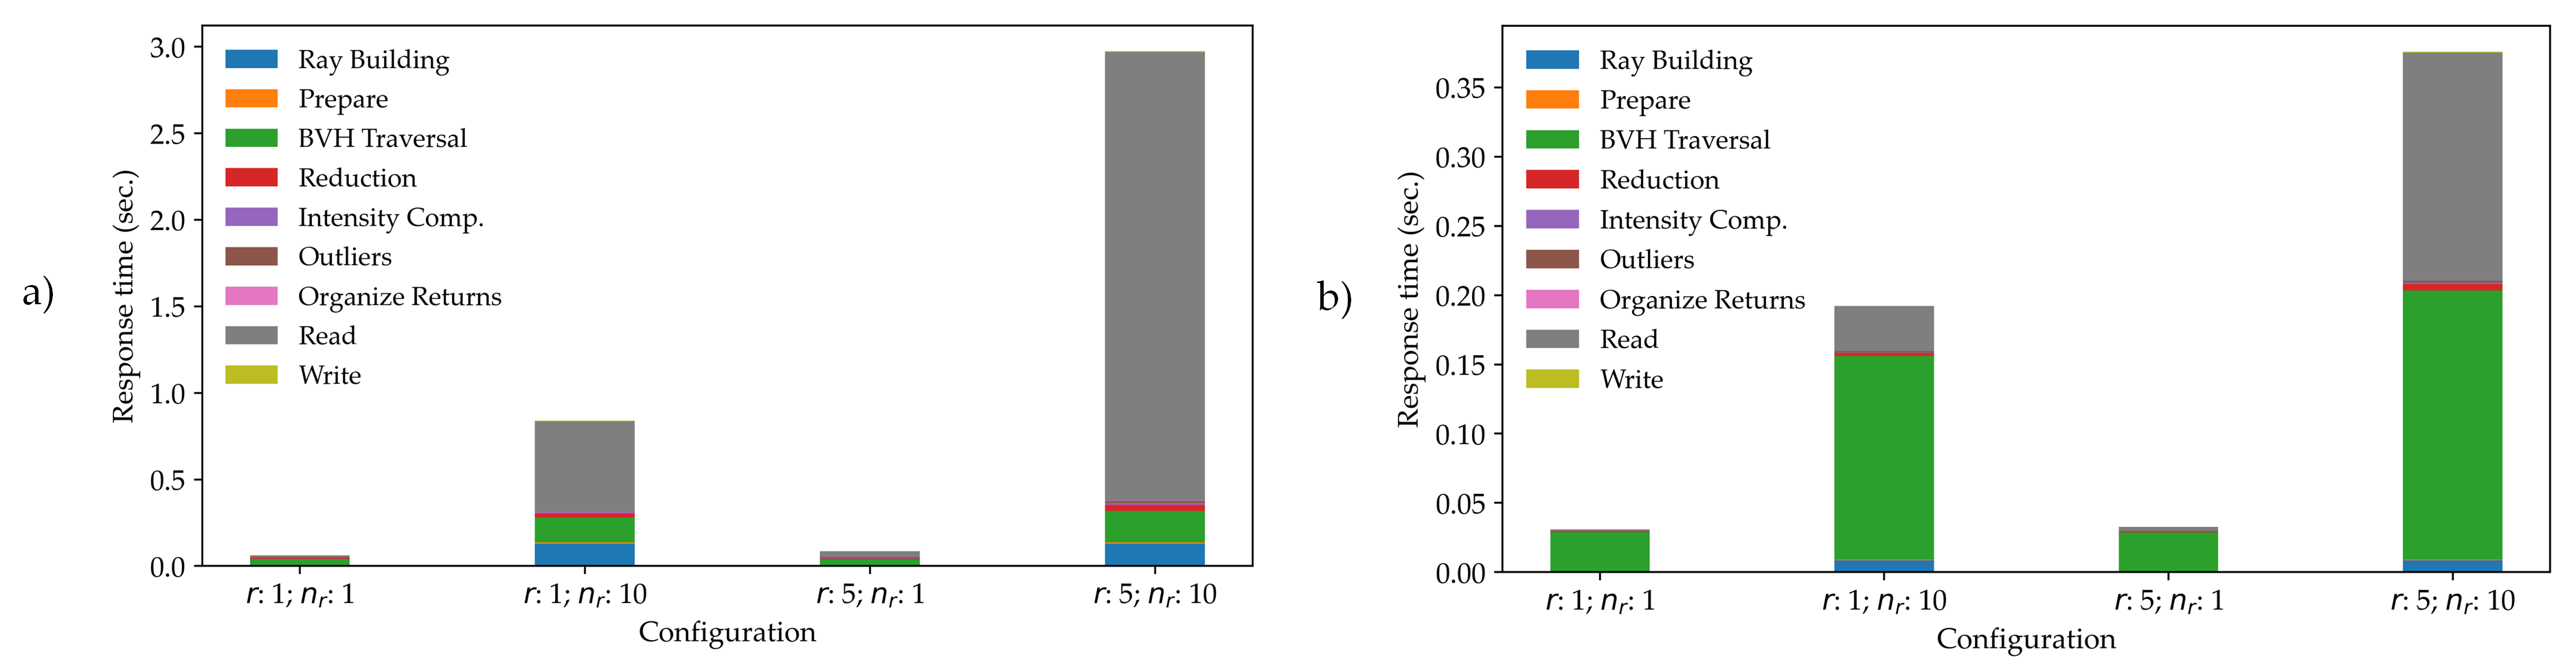
\includegraphics[width=\linewidth]{figs/lidar_simulation/lidar_response_time_stage.png}
	\caption{Absolute (left) and relative (right) response time of LiDAR stages. a) The first chart row compares the performance of TLS in a procedural forest, using a different number of allowed returns ($r$) and rays within a pulse ($n_r$). Similarly to TLS, the second chart row presents the results for an ALS sensor. The first row of the right chart is linked to the first column in the left chart.}
	\label{fig:lidar_response_time_chart}
\end{figure*}

\textbf{Stage occupancy}. In addition to the overall response time, the individual latency of each stage within the simulation kernel was also measured. To this end, each stage was explicitly synchronized in the CPU instead of allowing OpenGL to handle parallelism and memory access. Figure \ref{fig:lidar_response_time_chart} shows the relative latency for some complex configurations, using environments of lower (5M) and higher complexity (10M), scanned with 5M pulses. Besides the LiDAR phases depicted in Figure \ref{fig:lidar_workflow}, reading is also considered as it is needed either to perform further processing or to store the returned point cloud. Instead of computing the whole ray buffer at once, rays were iteratively constructed to avoid CPU and GPU data transfers.

As reported, transferring collisions to the CPU takes a substantial portion of time, whereas BVH traversal is notably more complex for highly populated environments. However, traversing a scene is significantly slower for TLS setups as they cannot discard clusters as rapidly. The reduction stage is also relevant in this chart as a result of the pulse handling. Rays within a pulse are managed by the same thread, instead of one per ray. 

\subsection{Generation of synthetic datasets}

Another main objective of this work is to provide a framework for generating large semantic datasets. Thus, several tests have been conducted to evaluate both the dimensionality and the number of labels in the collected datasets. Comparisons were established with previously cited work \cite{yue_lidar_2018, xiao_synlidar_2021, behley_towards_2021, pan_semanticposs_2020, caesar_nuscenes_2020}, either based on real or synthetic datasets, by taking into account the number of scans, the overall number of points, as well as the number of semantic annotations. To provide a fair evaluation, the tests were performed using the configuration of a Velodyne HDL-64E \cite{su_simulation_2019}, as proposed in most of the urban datasets in the literature \cite{behley_towards_2021, xiao_synlidar_2021, caesar_nuscenes_2020}. Aerial surveys are, on the other hand, not frequent in previous work, and their importance must also be highlighted. Accordingly, we have also performed simulations using the configuration of an airborne DJI Zenmuse L1 sensor \cite{dji_zenmuse_2020}. Remark that some of the sensor parameters are not provided by the manufacturers, and thus they have been adjusted to generate dense points clouds (Table \ref{table:test_sensor_parameters}). Also, the heterogeneous height of urban environments required solving the entire scan in multiple steps with different heights.

\renewcommand{\arraystretch}{1.1}
\begin{table*}
    \centering
    \caption{Overview of outdoor LiDAR datasets with semantic annotations, regarding their average size ($\textit{Points} / \textit{Scans}$) and number of classes ($\textit{Labels}$).}
    \label{table:lidar_dataset_comparison}
    \centering
    \begin{tabular}{lrrrrr}
    \hline
    \textbf{Dataset} & \textbf{Annotation} & \textbf{\#Scans} & \textbf{Average size} & \textbf{Labels} & \textbf{Synthetic}\\
    \midrule
    SynLiDAR \cite{xiao_synlidar_2021} & Point-wise & 198,396 & 98.197k points & 32 & \cmark \\
    GTA-LiDAR \cite{yue_lidar_2018} & Pixel-wise & 121,087 & - & 2 & \cmark \\
    Semantic3D \cite{hackel_semantic3d_2017} & Point-wise & 30 & \textbf{133.3M} points & 8 & \xmark \\
    SemanticKITTI \cite{behley_towards_2021} & Point-wise & 43,552 & 105.79k points & 25 & \xmark \\
    SemanticPOSS \cite{pan_semanticposs_2020} & Point-wise & 2,988 & 72.289k points & 14 & \xmark \\
    nuScenes \cite{caesar_nuscenes_2020} & Point-wise & 40,000 & 35k points & 32 & \xmark \\
    \midrule
    Ours & Point-wise & 488 & 622.95k points & \textbf{53} & \cmark \\
    \bottomrule
    \end{tabular}
\end{table*}

The results are collected by scanning two virtual urban scenes. The first has 32 semantic classes, whereas the second environment presents 45 semantic annotations. Furthermore, these scenes were populated with procedural pedestrians and vehicles. After scanning both environments, an average frame size of nearly 623k points was reported from 488 scans, either from TLS or ALS, which greatly improves the current average size of synthetic LiDAR simulators. Despite real-world datasets acquiring more dense point clouds, e.g., Semantic3D \cite{hackel_semantic3d_2017}, the main contribution of virtual scans is their low response time and efficiency both in acquiring data and annotating each point. Furthermore, the conducted tests were only performed over procedural environments generated with a single seed. Otherwise, a large number of differently populated environments could be modelled to further collect synthetic LiDAR datasets.

Figure \ref{fig:semantic_histogram} illustrates semantic labels linked to 3D models as well as the result from TLS and ALS scans, coloured with their height. The number of points annotated with each category is depicted using bar charts, by reporting points returned from TLS and the fusion of both TLS and ALS (Table \ref{table:lidar_dataset_comparison}). Despite the contribution of ALS scans being relevant for augmenting the dataset labels, its weight on the bar chart is reduced due to the relatively low number of rays in comparison with TLS scans.

\begin{figure*}
    \centering
    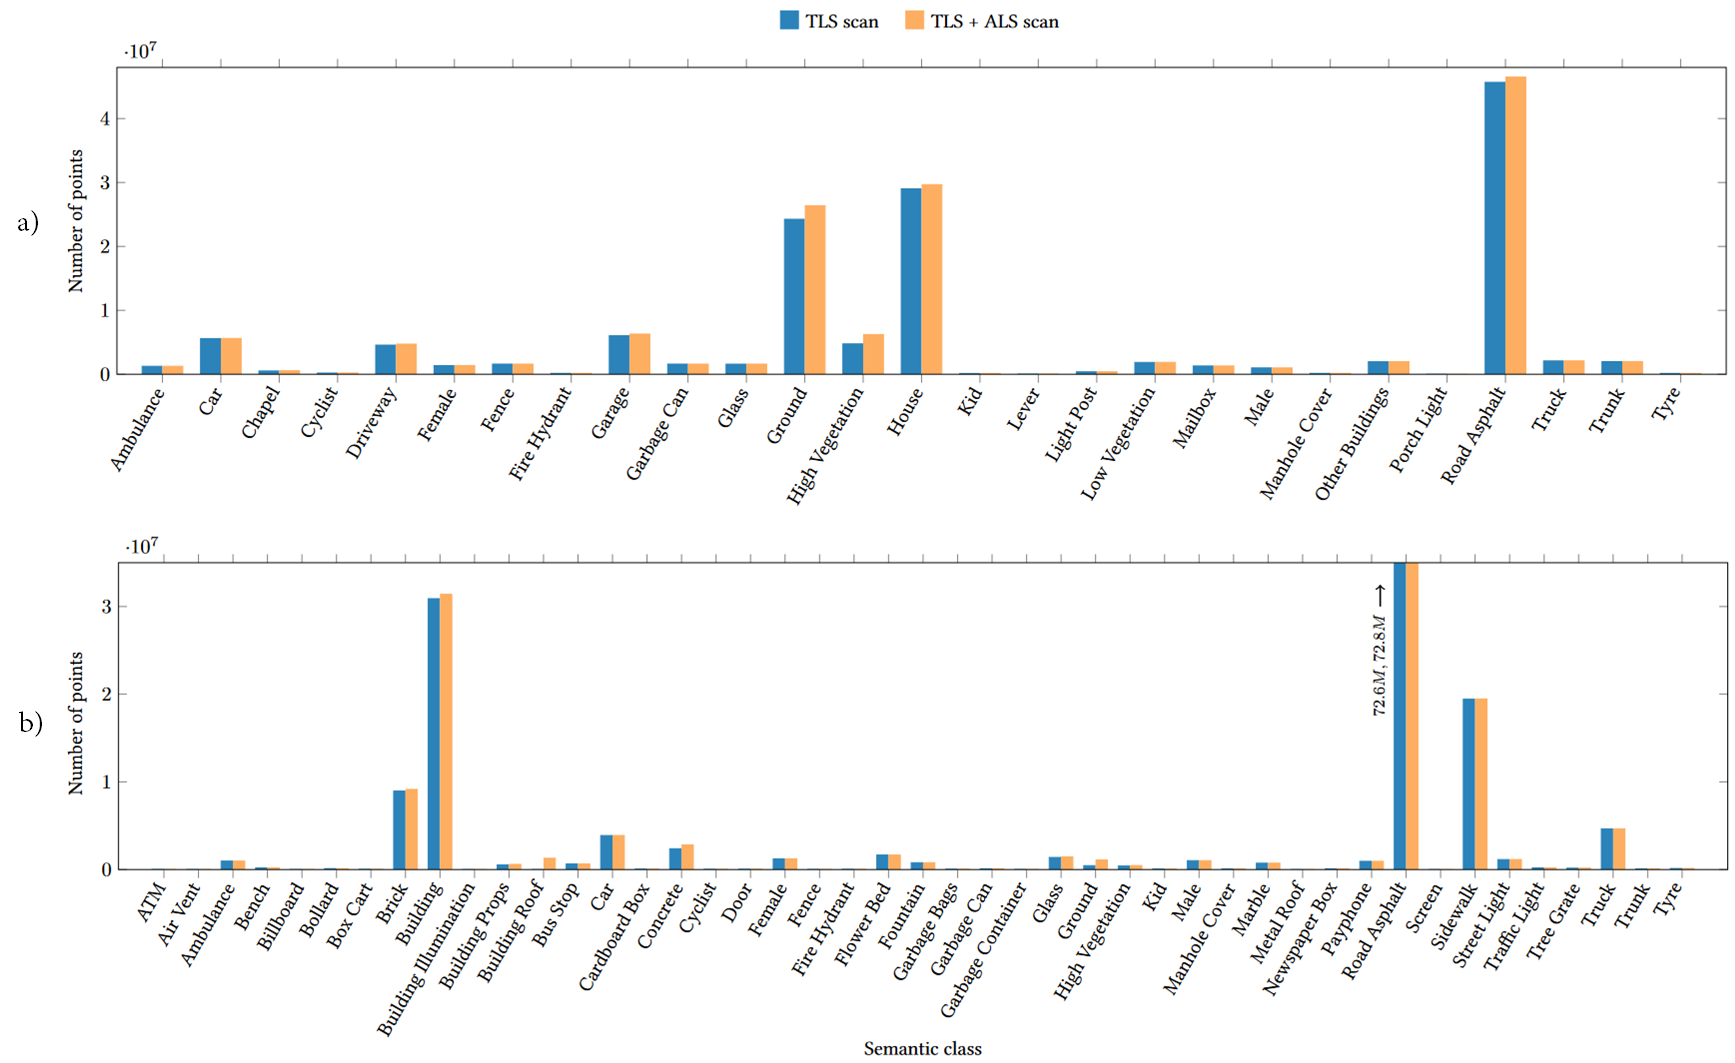
\includegraphics[width=\linewidth]{figs/lidar_simulation/bar_chart_annotations.png}
	\caption{Number of LiDAR points per semantic label in two different urban environments. The first bar reports the results of TLS scans, whereas the second bar shows the results combining both ALS and TLS. a) Distribution of 139M points and 145M points for TLS and TLS + ALS scans, respectively, whereas b) shows the profile generated by 165M and 170M points. }
	\label{fig:semantic_histogram}
\end{figure*}

\renewcommand{\arraystretch}{1.2}
\begin{table*}
    \caption{Specifications of sensors simulated during the scanning of urban environments. Parameters corresponding solely to virtual scanning are highlighted in cursive.}
    \label{table:test_sensor_parameters}
    \centering
    \begin{tabular}{lcccc}
    \hline
     & \multicolumn{4}{c}{\textbf{Sensors}}\\
    \cmidrule{2-5}
    \textbf{Attributes} & \multicolumn{2}{c}{\textbf{Velodyne HDL-64E} \cite{su_simulation_2019}} & \multicolumn{2}{c}{\textbf{Zenmuse L1} \cite{dji_zenmuse_2020}}\\
    \cmidrule{2-5}
     & Environment 1 & Environment 2 & Environment 1 & Environment 2\\
    \midrule
    Field of view & \multicolumn{2}{c}{360\textdegree $\times$ 26,9\textdegree} & \multicolumn{2}{c}{70,4\textdegree $\times$ 4,5\textdegree}\\
    Resolution & \multicolumn{2}{c}{0,08\textdegree $\times$ 0,4\textdegree} & \multicolumn{2}{c}{~0,1437\textdegree $\times$ 0.00918\textdegree}\\
    Number of channels & \multicolumn{2}{c}{64} & \multicolumn{2}{c}{1}\\
    Vertical FOV origin & \multicolumn{2}{c}{-11,45\textdegree} & \multicolumn{2}{c}{0\textdegree}\\
    Maximum range & \multicolumn{2}{c}{120 \si{\meter}} & \multicolumn{2}{c}{190 \si{\meter}}\\
    Maximum number of returns & \multicolumn{2}{c}{2} & \multicolumn{2}{c}{3}\\
    Scan altitude* ($h_{l}$) & \multicolumn{2}{c}{2 \si{\meter}} & 45 \si{\meter} & 115 \si{\meter} / 290 \si{\meter}\\
    Platform speed* ($s_{p}$) & \multicolumn{2}{c}{--} & \multicolumn{1}{c}{2 \si{\meter}/\si{\second}} & 0.5 \si{\meter}/\si{\second}\\
    Rays within a pulse* ($n_{r}$) & \multicolumn{2}{c}{5} & \multicolumn{2}{c}{5}\\
    \midrule
    Pulses per scan* & \multicolumn{2}{c}{302,625} & \multicolumn{2}{c}{240,000}\\
    \midrule
    Generated rays & 342M & 30M & 390M & 72M\\
    Resulting points & 139M & 5,5M & 165M & 5M\\
    \bottomrule
    \end{tabular}\\
    \footnotesize{$^*$ These parameters were not provided by the manufacturer and thus were adjusted to each scenario to provide a dense result.}\\
\end{table*}
\renewcommand{\arraystretch}{1}

\subsection{Visual results}

Besides quantitative tests, comparison can also be established with visual results using a real LiDAR point cloud as the baseline result. Furthermore, these tests are performed over CAD models rather than polygonal meshes extracted from previous scans, as they may introduce some errors in the geometry. Hence, CAD models of vehicles were easy to collect, which also happen to be very frequently scanned in publicly available TLS datasets. More specifically. Thus, the dataset obtained from a Pandar64 sensor \cite{hesai_pandaset_2021} was used, which also provided RGB images and individual TLS scans. The latter is relevant as it allows comparing single scans instead of one composed of several scans obtained from different viewpoints. 

Regarding other virtual simulators, most of the revised work provides datasets rather than the simulator itself, operates only in pre-defined environments \cite{lg_electronics_rd_lab_lgsvl_2021}, or do not integrate surface materials \cite{yue_lidar_2018, xiao_synlidar_2021, manivasagam_lidarsim_2020, fang_augmented_2020, su_simulation_2019}. Others lack non-uniform scanning \cite{dosovitskiy_carla_2017} and noise/loss behavior \cite{shah_airsim_2017}. Consequently, comparisons have been performed against the widespread blender plugin Blensor \cite{gschwandtner_blensor_2011}; it is an open-source project that also provides a naïve simulation of noise and errors derived from reflective surfaces. The scenario was configured so that car objects were marked with different reflectivity factors, whereas LiDAR sensors were located according to the real LiDAR placement. Glass materials were simulated with a mirror-like surface behaviour. Regarding scanning resolution, the Pandar64 sensor presents different spatial resolutions along the vertical axis. In contrast to previous work, the proposed solution also supports the nonuniform vertical resolution. Finally, a loss function was defined for glossy surfaces, over which reflection errors were emulated. Still, the effects of the 'time-walk' effect are limited due to the reduced distance between the measuring platform and the target surface. 

Figure \ref{fig:lidar_point_cloud_comparison} shows that glossy surfaces are omitted by Blensor, whereas our point clouds present some gaps as a result of the loss function. On the other hand, Blensor includes a noise function defined by its amplitude and distribution to include some variability in the final point cloud. Consequently, both virtual LiDAR sensors generate results following patterns similar to the real LiDAR, including noisy point clouds; however, reflection errors were better emulated by the proposed solution, yet notably improving the response time.

\begin{figure*}
    \centering
    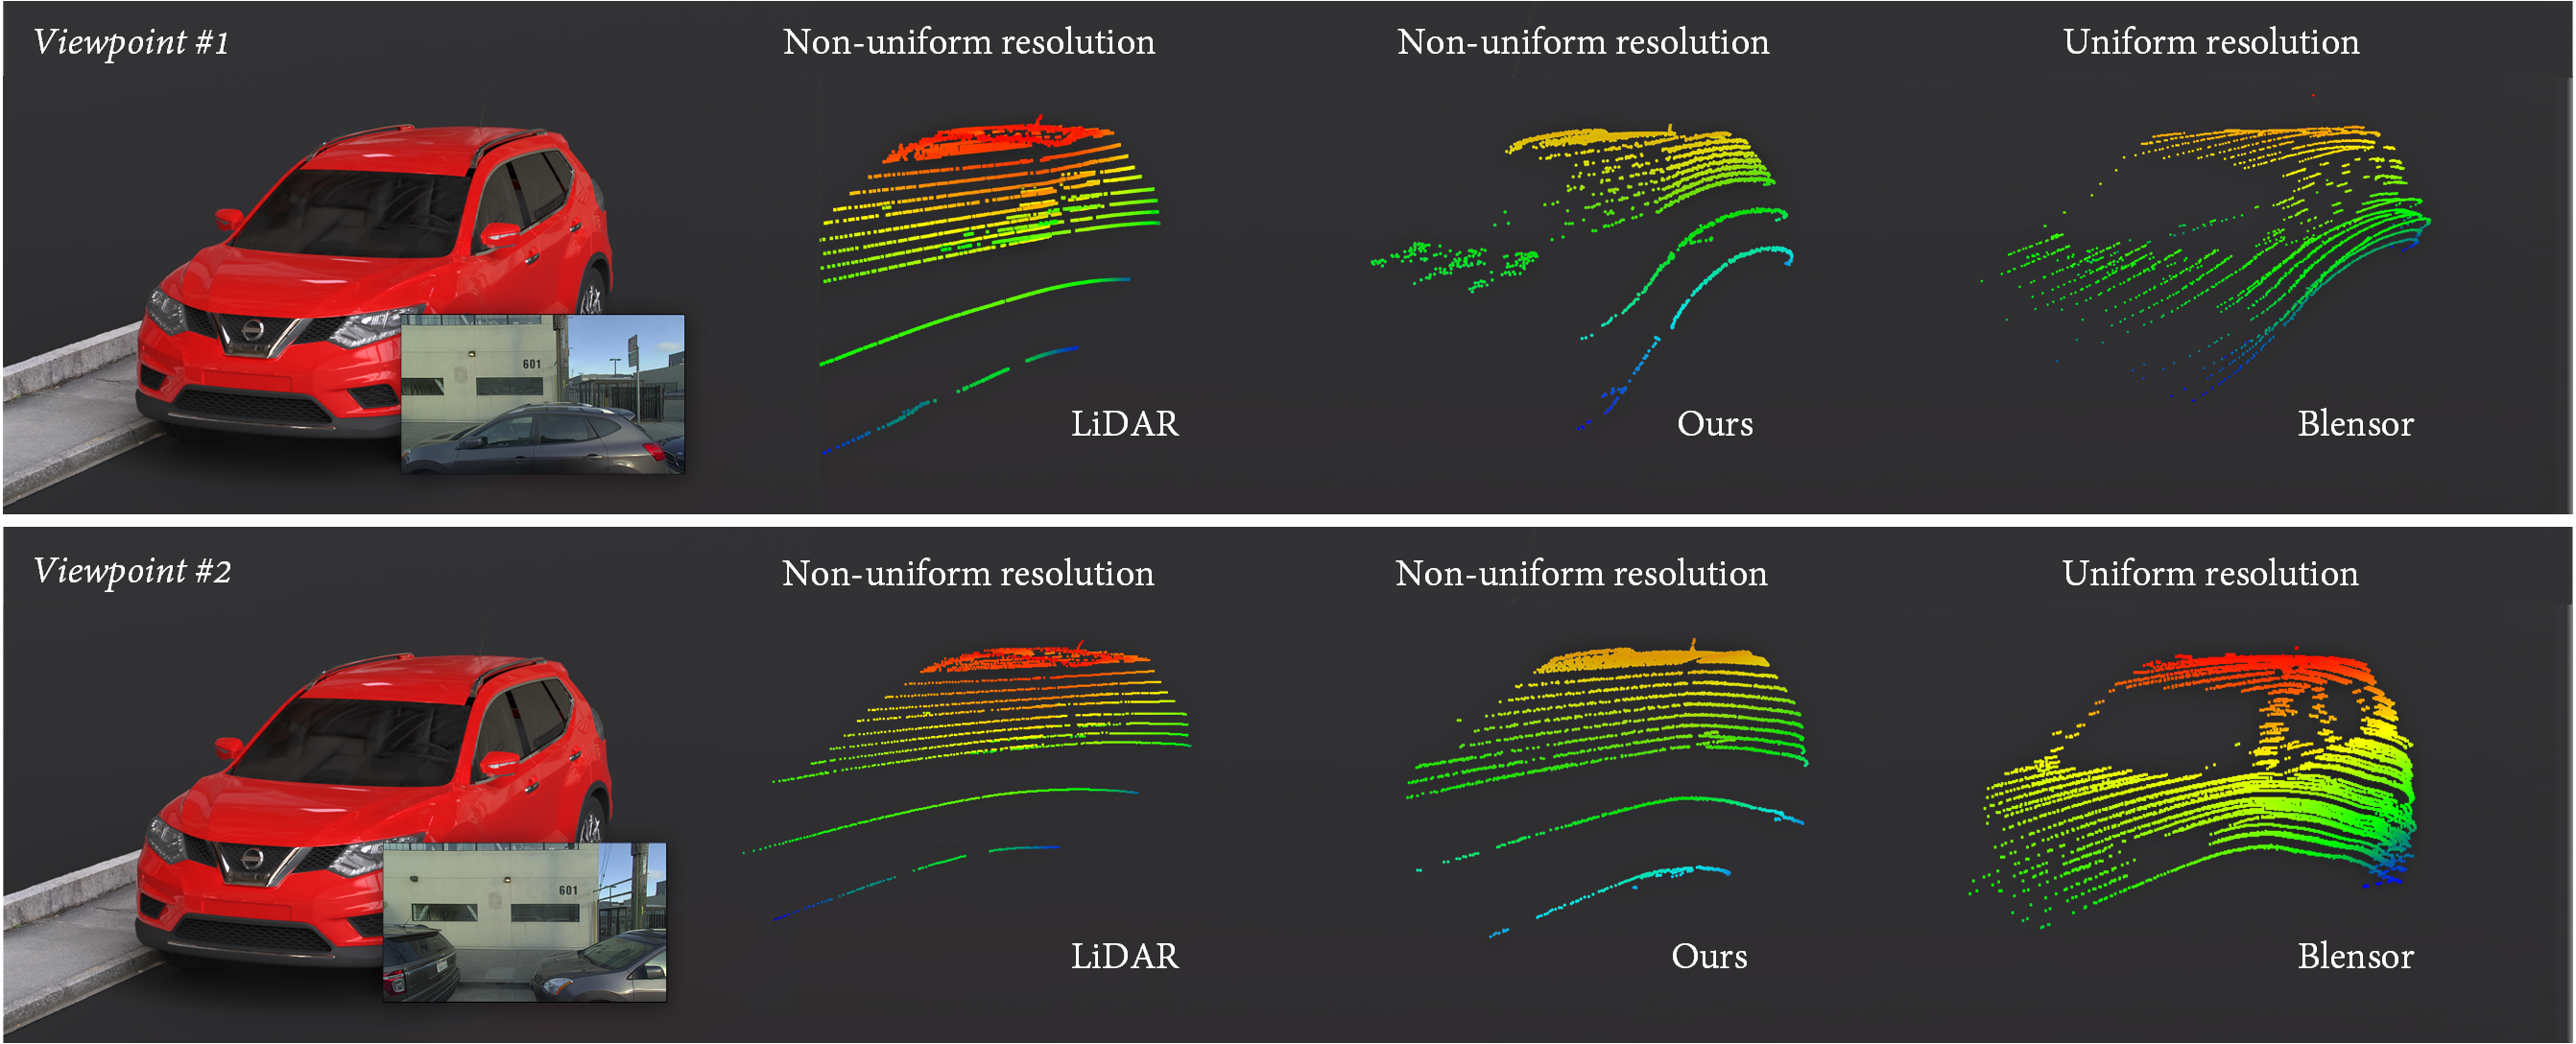
\includegraphics[width=\linewidth]{figs/lidar_simulation/lidar_point_cloud_comparison.png}
	\caption{Comparison of real and synthetic point clouds. The first two images depict the input CAD model and its corresponding LiDAR point cloud as captured from a Pandar64 sensor \cite{hesai_pandaset_2021}. The third image illustrates a synthetic point cloud from our simulator, and finally, the fourth image shows the result from the Blensor plugin with a uniform vertical resolution. }
	\label{fig:lidar_point_cloud_comparison}
\end{figure*}

\section{Conclusions and future work}

A massively parallel and parameterized LiDAR was proposed for generating dense semantic point clouds, aimed at collecting large datasets for Deep Learning models. It operates over any environment defined as a triangle mesh; however, procedural scenes were constructed to provide a time-efficient alternative concerning the manual annotation task. These are labelled once and produce large datasets, whereas static environments only contribute to building one point cloud. Spatial queries were rapidly solved with state-of-the-art data structures proposed for ray tracing, whereas the proposed ToF solver includes multiple returns and well-known LiDAR errors. To this end, LiDAR's pulses were discretized as several rays that strike into the scene surfaces, instead of solving the simulation in the image space.  Thus, the described algorithm is suitable both for real-time simulations and the generation of large LiDAR semantic point clouds with low latency. Accordingly, LiDAR sessions can be solved iteratively or in a single batch. Also, the sensor parameterization helps in simulating a wide range of LiDAR sensors and platforms, including ALS.

This solution was assessed through its performance and capabilities in the generation of large datasets. The workflow was implemented in GLSL and compared with its analogous multi-core CPU approach by conducting much more dense scans than actual LiDAR sensors. These tests showed that the GPU approach improves the sequential procedure with speedups above 90\%. Hence, it was proved that this simulator is appropriate for generating large semantic LiDAR datasets with low latency, despite working with large and highly detailed scenes. Regarding scanning capabilities, a significant enhancement both in average scan size and the number of semantic labels was observed. Note that this is not solely affected by the LiDAR scans, but also by the facilities given on the annotation task. Finally, point clouds were compared against Blensor regarding their graphic results, after which was proven that some errors such as those derived from highly reflective surfaces were better simulated by our solution. 

In future work, the proposed pipeline could be further accelerated in multi-GPU systems. Furthermore, we aim to extend this framework to full-waveform and single-photon LiDAR \cite{tachella_real-time_2019} and other nonincluded systems. Regarding Deep Learning applications, a deeper study ought to be conducted to show the benefits of using virtual LiDAR over procedural environments in the generation of semantic LiDAR datasets.

\newcommand{\datasetImageHeight}{-.09\totalheight}
\newcommand{\datasetImageSize}{1.8cm}
\newcommand{\lidarCoreLabel}{ToF Solver}

\renewcommand{\arraystretch}{1.1}[hb]
\begin{table*}
    \small
    \centering
    \caption{Comparison of CPU and GPU performance for TLS and ALS scans. The response time is evaluated using both static and procedural scenes with a significant number of triangles.}
    \label{table:lidar_response_time}
    \begin{tabular}{c|c|c|llll}
    \toprule
    \multicolumn{7}{c}{\textbf{Terrestrial LiDAR}}\\
    \cmidrule{1-7}
    \multicolumn{3}{c}{\textbf{Configuration}} & &
    \raisebox{\datasetImageHeight}{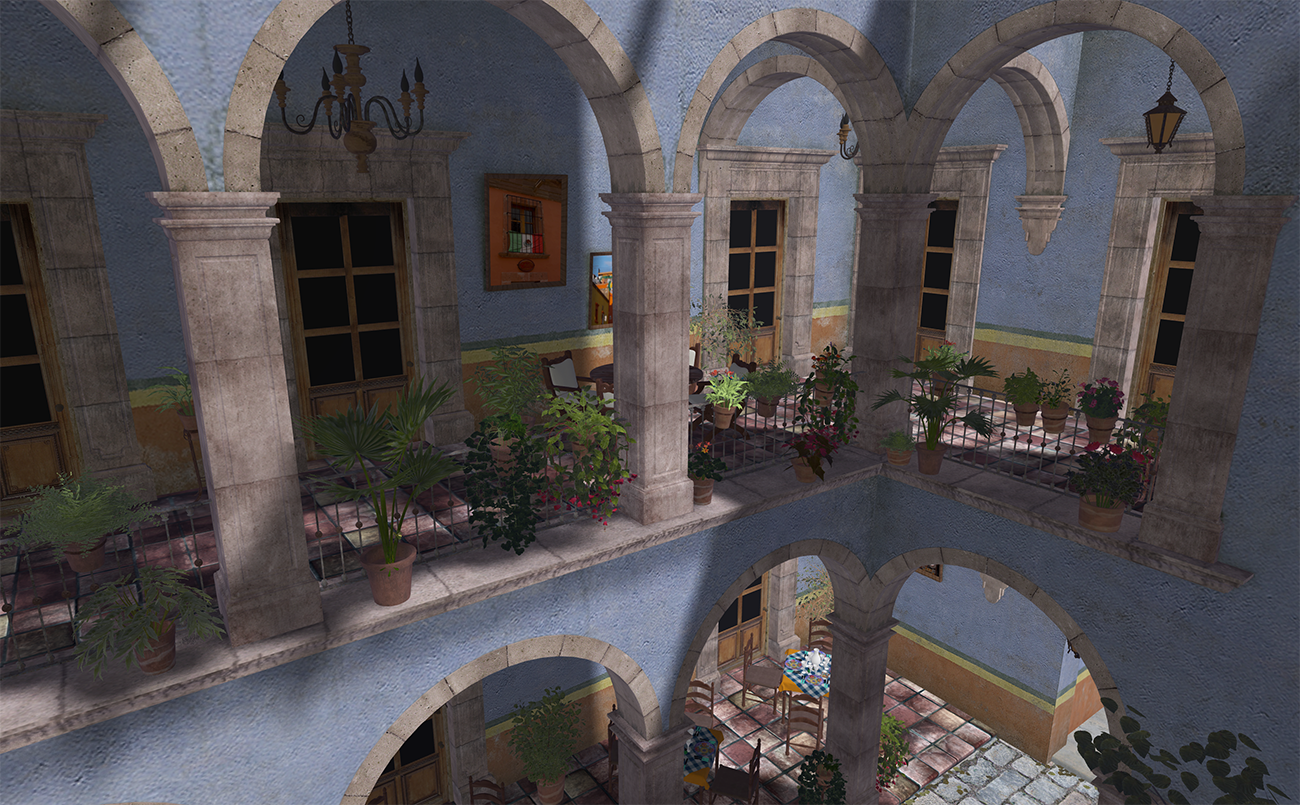
\includegraphics[width=\datasetImageSize]{figs/datasets/san_miguel.png}} \hspace{1mm}
    \shortstack{San Miguel\\ \#triangles\\ 5.6M } & \raisebox{\datasetImageHeight}{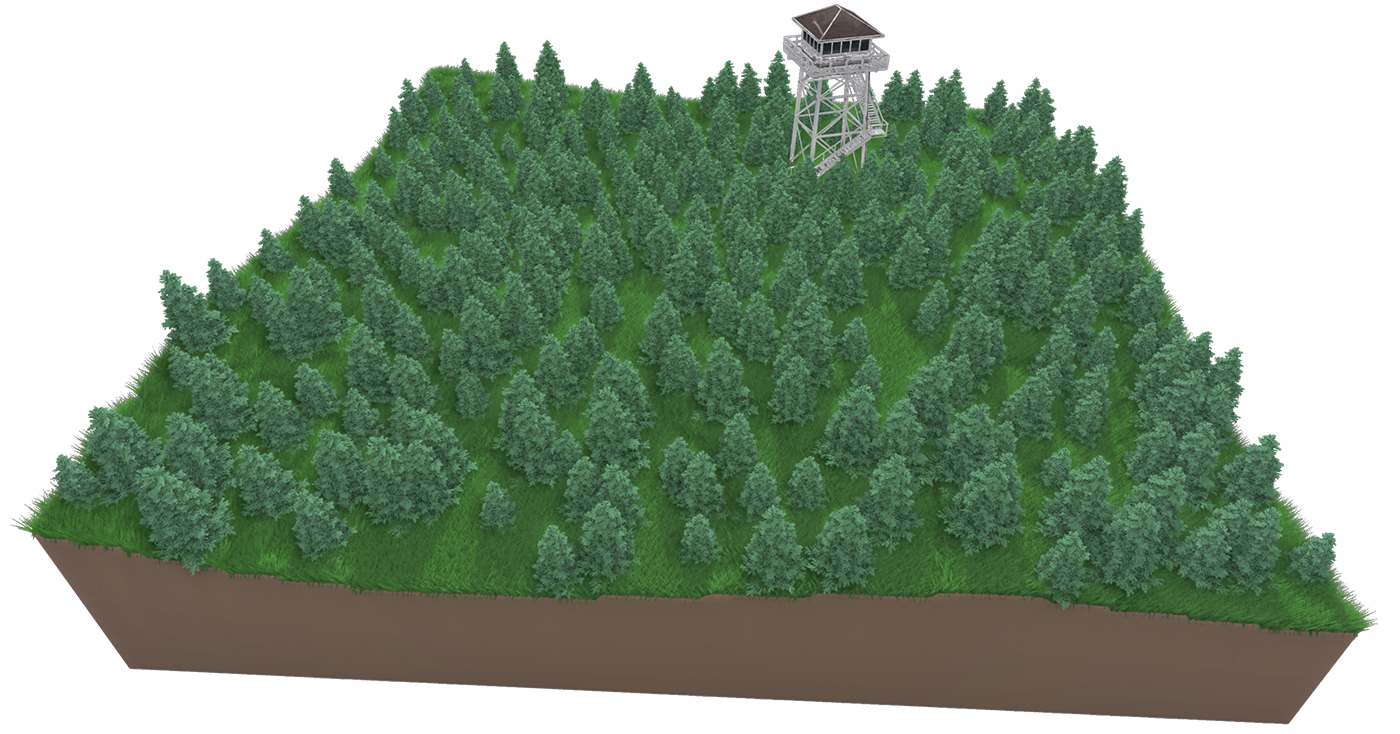
\includegraphics[width=\datasetImageSize]{figs/datasets/tls_forest.png}} \hspace{1mm}
    \shortstack{Forest\\ \#triangles\\ 11M } &
    \raisebox{\datasetImageHeight}{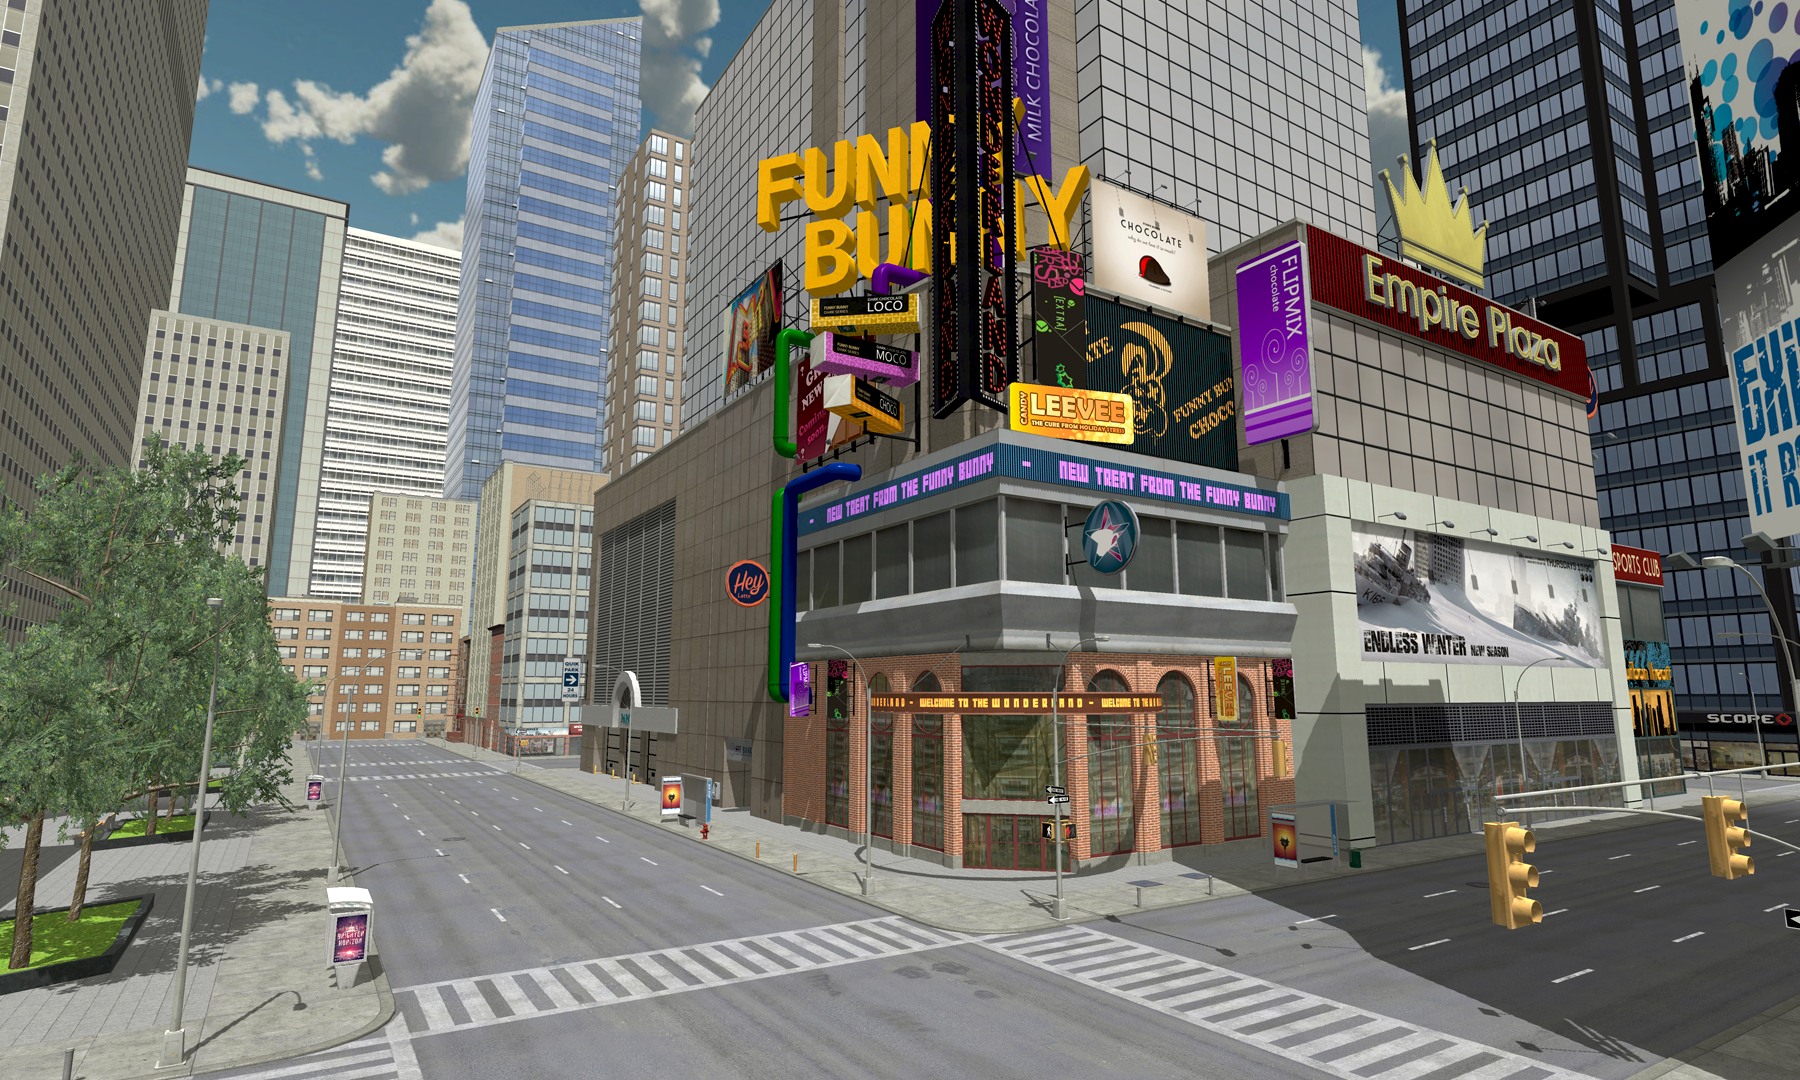
\includegraphics[width=\datasetImageSize]{figs/datasets/mcp.png}} \hspace{1mm}
    \shortstack{City\\ \#triangles\\ 10.1M }\\
    \cmidrule{1-7}
    \multicolumn{7}{c}{Single return}\\
    \cmidrule{1-7}
    \textbf{$n_{p}$} & Method & \textbf{$n_{r}$} & Ray inst. & \lidarCoreLabel & \lidarCoreLabel & \lidarCoreLabel\\
    \cmidrule{1-7}
    \multirow{2}{*}{5M} & \textbf{GPU} & \multirow{2}{*}{10} & 
    \textbf{0.141s} & \textbf{2.747s} & \textbf{0.755s} & \textbf{3.664s}\\ 
    & CPU & & 
    15.601s & 193.790s & 1,854.337 & 128.900s\\
    \cmidrule{1-7}
    \multirow{2}{*}{10M} & \textbf{GPU} & \multirow{2}{*}{10} & 
    \textbf{0,279s} & \textbf{5.254s} & \textbf{1.510s} & \textbf{7.745s}\\ 
    & CPU & & 
    31.740s & 1,571.758s & 3,743.797s & 261.091s\\
    \toprule
    \multicolumn{7}{c}{Multiple returns (5)}\\
    \cmidrule{1-7}
    \multirow{2}{*}{5M} & \textbf{GPU} & \multirow{2}{*}{10} & 
    \textbf{0,141s} & \textbf{5.637s} & \textbf{3.323s} & \textbf{6.597s}\\ 
    & CPU & & 
    15,601s & 194,533s & 1.900,348s & 129,725s\\
    \cmidrule{1-7}
    \multirow{2}{*}{10M} & \textbf{GPU} & \multirow{2}{*}{10} & 
    \textbf{0.279s} & \textbf{11.481s} & \textbf{6.906s} & \textbf{12.949s}\\ 
    & CPU & & 
    31.740s & 1,573.349s & 3,748.547s & 262.640s\\
    \bottomrule
    \toprule
    \multicolumn{7}{c}{\textbf{Aerial LiDAR}}\\
    \cmidrule{1-7}
    \multicolumn{3}{c|}{\textbf{Configuration}} & &
    \raisebox{\datasetImageHeight}{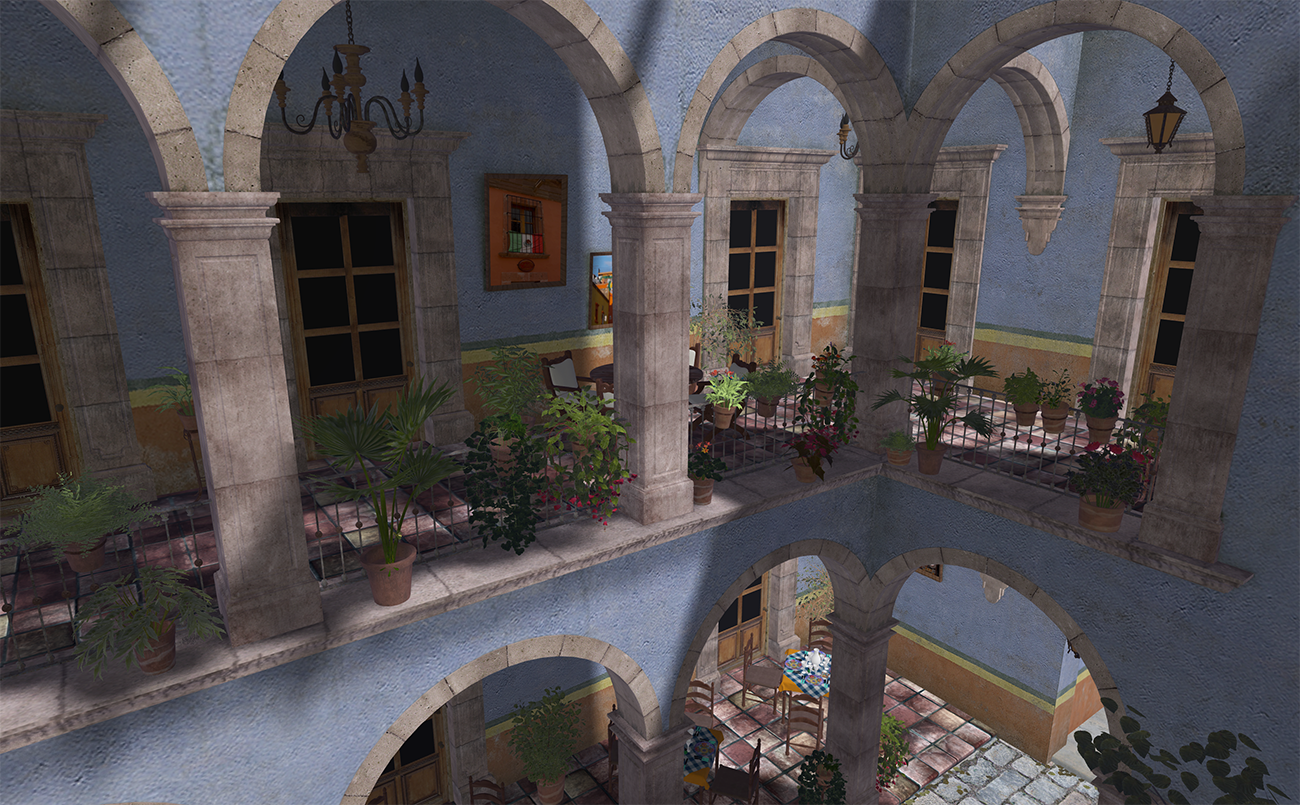
\includegraphics[width=\datasetImageSize]{figs/datasets/san_miguel.png}} \hspace{1mm}
    \shortstack{San Miguel\\ \#triangles\\ 5.6M } & \raisebox{\datasetImageHeight}{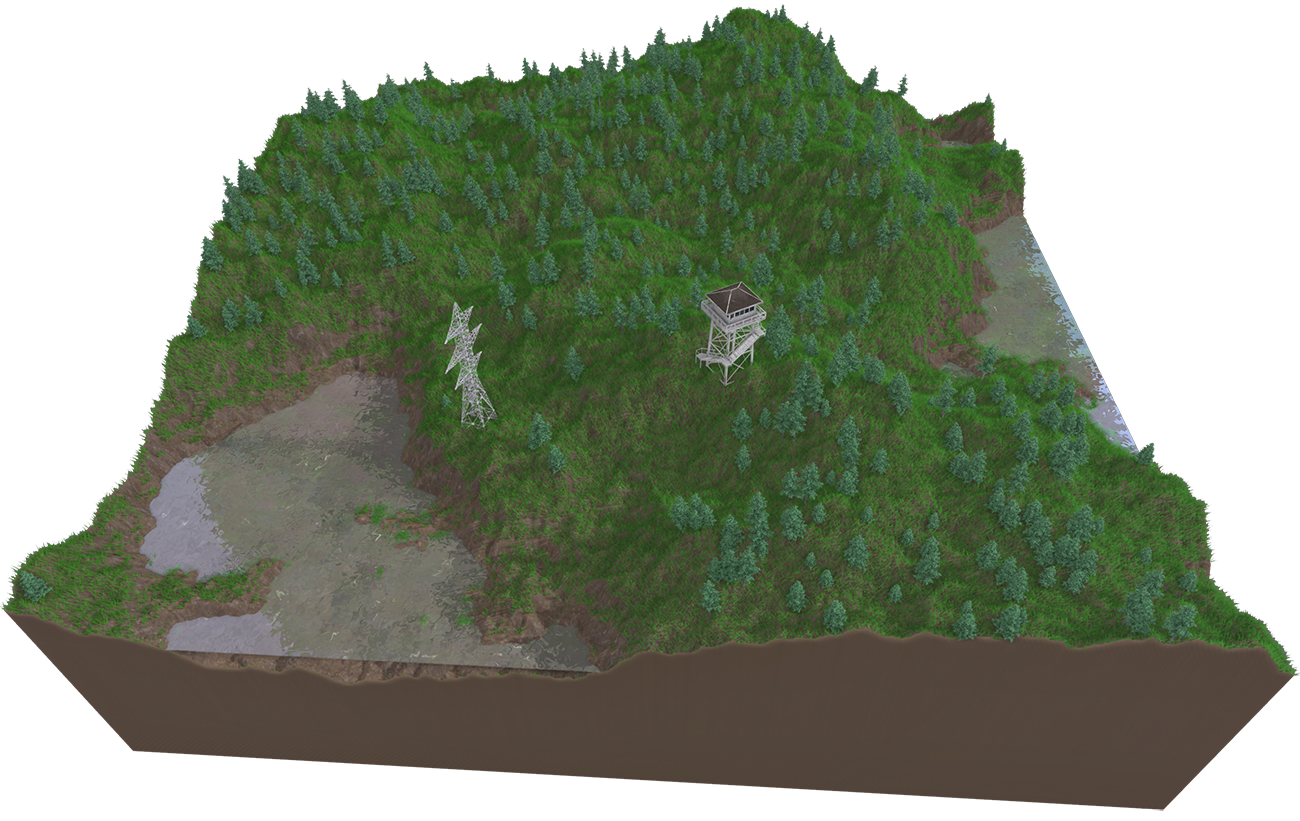
\includegraphics[width=\datasetImageSize]{figs/datasets/als_forest.png}} \hspace{1mm}
    \shortstack{Forest\\ \#triangles\\ 11M } &
    \raisebox{\datasetImageHeight}{\includegraphics[width=\datasetImageSize]{figs/datasets/suburb.png}} \hspace{1mm}
    \shortstack{Suburb\\ \#triangles\\ 4.1M }\\
    \cmidrule{1-7}
    \multicolumn{7}{c}{Multiple returns (5)}\\
    \cmidrule{1-7}
    \multirow{2}{*}{5M} & \textbf{GPU} & \multirow{2}{*}{10} & 
    \textbf{1.240s} & \textbf{0.923s} & \textbf{2.348s} & \textbf{0.995s}\\ 
    & CPU & & 
    12.586s & 66.889s & 102.070s & 119.946s\\
    \cmidrule{1-7}
    \multirow{2}{*}{10M} & \textbf{GPU} & \multirow{2}{*}{10} & 
    \textbf{2.510s} & \textbf{1.806s} & \textbf{4.4294s} & \textbf{1.996s}\\ 
    & CPU & & 
    27.583s & 131.253s & 344.882s & 235.174s\\
    \bottomrule
    \end{tabular}
    \libertineNormal
\end{table*}
\renewcommand{\arraystretch}{1}